% Options for packages loaded elsewhere
\PassOptionsToPackage{unicode}{hyperref}
\PassOptionsToPackage{hyphens}{url}
\PassOptionsToPackage{dvipsnames,svgnames,x11names}{xcolor}
%
\documentclass[
  11pt,
  a4paper,
]{article}

\usepackage{amsmath,amssymb}
\usepackage{iftex}
\ifPDFTeX
  \usepackage[T1]{fontenc}
  \usepackage[utf8]{inputenc}
  \usepackage{textcomp} % provide euro and other symbols
\else % if luatex or xetex
  \usepackage{unicode-math}
  \defaultfontfeatures{Scale=MatchLowercase}
  \defaultfontfeatures[\rmfamily]{Ligatures=TeX,Scale=1}
\fi
\usepackage[]{libertinus}
\ifPDFTeX\else  
    % xetex/luatex font selection
    \setmonofont[Scale=0.92]{Latin Modern Mono}
\fi
% Use upquote if available, for straight quotes in verbatim environments
\IfFileExists{upquote.sty}{\usepackage{upquote}}{}
\IfFileExists{microtype.sty}{% use microtype if available
  \usepackage[]{microtype}
  \UseMicrotypeSet[protrusion]{basicmath} % disable protrusion for tt fonts
}{}
\makeatletter
\@ifundefined{KOMAClassName}{% if non-KOMA class
  \IfFileExists{parskip.sty}{%
    \usepackage{parskip}
  }{% else
    \setlength{\parindent}{0pt}
    \setlength{\parskip}{6pt plus 2pt minus 1pt}}
}{% if KOMA class
  \KOMAoptions{parskip=half}}
\makeatother
\usepackage{xcolor}
\usepackage[a4paper,textheight=24cm,textwidth=15.5cm]{geometry}
\setlength{\emergencystretch}{3em} % prevent overfull lines
\setcounter{secnumdepth}{5}
% Make \paragraph and \subparagraph free-standing
\makeatletter
\ifx\paragraph\undefined\else
  \let\oldparagraph\paragraph
  \renewcommand{\paragraph}{
    \@ifstar
      \xxxParagraphStar
      \xxxParagraphNoStar
  }
  \newcommand{\xxxParagraphStar}[1]{\oldparagraph*{#1}\mbox{}}
  \newcommand{\xxxParagraphNoStar}[1]{\oldparagraph{#1}\mbox{}}
\fi
\ifx\subparagraph\undefined\else
  \let\oldsubparagraph\subparagraph
  \renewcommand{\subparagraph}{
    \@ifstar
      \xxxSubParagraphStar
      \xxxSubParagraphNoStar
  }
  \newcommand{\xxxSubParagraphStar}[1]{\oldsubparagraph*{#1}\mbox{}}
  \newcommand{\xxxSubParagraphNoStar}[1]{\oldsubparagraph{#1}\mbox{}}
\fi
\makeatother

\usepackage{color}
\usepackage{fancyvrb}
\newcommand{\VerbBar}{|}
\newcommand{\VERB}{\Verb[commandchars=\\\{\}]}
\DefineVerbatimEnvironment{Highlighting}{Verbatim}{commandchars=\\\{\}}
% Add ',fontsize=\small' for more characters per line
\newenvironment{Shaded}{}{}
\newcommand{\AlertTok}[1]{\textcolor[rgb]{1.00,0.33,0.33}{\textbf{#1}}}
\newcommand{\AnnotationTok}[1]{\textcolor[rgb]{0.42,0.45,0.49}{#1}}
\newcommand{\AttributeTok}[1]{\textcolor[rgb]{0.84,0.23,0.29}{#1}}
\newcommand{\BaseNTok}[1]{\textcolor[rgb]{0.00,0.36,0.77}{#1}}
\newcommand{\BuiltInTok}[1]{\textcolor[rgb]{0.84,0.23,0.29}{#1}}
\newcommand{\CharTok}[1]{\textcolor[rgb]{0.01,0.18,0.38}{#1}}
\newcommand{\CommentTok}[1]{\textcolor[rgb]{0.42,0.45,0.49}{#1}}
\newcommand{\CommentVarTok}[1]{\textcolor[rgb]{0.42,0.45,0.49}{#1}}
\newcommand{\ConstantTok}[1]{\textcolor[rgb]{0.00,0.36,0.77}{#1}}
\newcommand{\ControlFlowTok}[1]{\textcolor[rgb]{0.84,0.23,0.29}{#1}}
\newcommand{\DataTypeTok}[1]{\textcolor[rgb]{0.84,0.23,0.29}{#1}}
\newcommand{\DecValTok}[1]{\textcolor[rgb]{0.00,0.36,0.77}{#1}}
\newcommand{\DocumentationTok}[1]{\textcolor[rgb]{0.42,0.45,0.49}{#1}}
\newcommand{\ErrorTok}[1]{\textcolor[rgb]{1.00,0.33,0.33}{\underline{#1}}}
\newcommand{\ExtensionTok}[1]{\textcolor[rgb]{0.84,0.23,0.29}{\textbf{#1}}}
\newcommand{\FloatTok}[1]{\textcolor[rgb]{0.00,0.36,0.77}{#1}}
\newcommand{\FunctionTok}[1]{\textcolor[rgb]{0.44,0.26,0.76}{#1}}
\newcommand{\ImportTok}[1]{\textcolor[rgb]{0.01,0.18,0.38}{#1}}
\newcommand{\InformationTok}[1]{\textcolor[rgb]{0.42,0.45,0.49}{#1}}
\newcommand{\KeywordTok}[1]{\textcolor[rgb]{0.84,0.23,0.29}{#1}}
\newcommand{\NormalTok}[1]{\textcolor[rgb]{0.14,0.16,0.18}{#1}}
\newcommand{\OperatorTok}[1]{\textcolor[rgb]{0.14,0.16,0.18}{#1}}
\newcommand{\OtherTok}[1]{\textcolor[rgb]{0.44,0.26,0.76}{#1}}
\newcommand{\PreprocessorTok}[1]{\textcolor[rgb]{0.84,0.23,0.29}{#1}}
\newcommand{\RegionMarkerTok}[1]{\textcolor[rgb]{0.42,0.45,0.49}{#1}}
\newcommand{\SpecialCharTok}[1]{\textcolor[rgb]{0.00,0.36,0.77}{#1}}
\newcommand{\SpecialStringTok}[1]{\textcolor[rgb]{0.01,0.18,0.38}{#1}}
\newcommand{\StringTok}[1]{\textcolor[rgb]{0.01,0.18,0.38}{#1}}
\newcommand{\VariableTok}[1]{\textcolor[rgb]{0.89,0.38,0.04}{#1}}
\newcommand{\VerbatimStringTok}[1]{\textcolor[rgb]{0.01,0.18,0.38}{#1}}
\newcommand{\WarningTok}[1]{\textcolor[rgb]{1.00,0.33,0.33}{#1}}

\providecommand{\tightlist}{%
  \setlength{\itemsep}{0pt}\setlength{\parskip}{0pt}}\usepackage{longtable,booktabs,array}
\usepackage{calc} % for calculating minipage widths
% Correct order of tables after \paragraph or \subparagraph
\usepackage{etoolbox}
\makeatletter
\patchcmd\longtable{\par}{\if@noskipsec\mbox{}\fi\par}{}{}
\makeatother
% Allow footnotes in longtable head/foot
\IfFileExists{footnotehyper.sty}{\usepackage{footnotehyper}}{\usepackage{footnote}}
\makesavenoteenv{longtable}
\usepackage{graphicx}
\makeatletter
\def\maxwidth{\ifdim\Gin@nat@width>\linewidth\linewidth\else\Gin@nat@width\fi}
\def\maxheight{\ifdim\Gin@nat@height>\textheight\textheight\else\Gin@nat@height\fi}
\makeatother
% Scale images if necessary, so that they will not overflow the page
% margins by default, and it is still possible to overwrite the defaults
% using explicit options in \includegraphics[width, height, ...]{}
\setkeys{Gin}{width=\maxwidth,height=\maxheight,keepaspectratio}
% Set default figure placement to htbp
\makeatletter
\def\fps@figure{htbp}
\makeatother
% definitions for citeproc citations
\NewDocumentCommand\citeproctext{}{}
\NewDocumentCommand\citeproc{mm}{%
  \begingroup\def\citeproctext{#2}\cite{#1}\endgroup}
\makeatletter
 % allow citations to break across lines
 \let\@cite@ofmt\@firstofone
 % avoid brackets around text for \cite:
 \def\@biblabel#1{}
 \def\@cite#1#2{{#1\if@tempswa , #2\fi}}
\makeatother
\newlength{\cslhangindent}
\setlength{\cslhangindent}{1.5em}
\newlength{\csllabelwidth}
\setlength{\csllabelwidth}{3em}
\newenvironment{CSLReferences}[2] % #1 hanging-indent, #2 entry-spacing
 {\begin{list}{}{%
  \setlength{\itemindent}{0pt}
  \setlength{\leftmargin}{0pt}
  \setlength{\parsep}{0pt}
  % turn on hanging indent if param 1 is 1
  \ifodd #1
   \setlength{\leftmargin}{\cslhangindent}
   \setlength{\itemindent}{-1\cslhangindent}
  \fi
  % set entry spacing
  \setlength{\itemsep}{#2\baselineskip}}}
 {\end{list}}
\usepackage{calc}
\newcommand{\CSLBlock}[1]{\hfill\break\parbox[t]{\linewidth}{\strut\ignorespaces#1\strut}}
\newcommand{\CSLLeftMargin}[1]{\parbox[t]{\csllabelwidth}{\strut#1\strut}}
\newcommand{\CSLRightInline}[1]{\parbox[t]{\linewidth - \csllabelwidth}{\strut#1\strut}}
\newcommand{\CSLIndent}[1]{\hspace{\cslhangindent}#1}

\usepackage{tikz}
\usepackage{xcolor}
\usepackage{tabularx}
\usepackage{orcidlink}
\usepackage{lineno}

\makeatletter
\@ifpackageloaded{caption}{}{\usepackage{caption}}
\AtBeginDocument{%
\ifdefined\contentsname
  \renewcommand*\contentsname{Table of contents}
\else
  \newcommand\contentsname{Table of contents}
\fi
\ifdefined\listfigurename
  \renewcommand*\listfigurename{List of Figures}
\else
  \newcommand\listfigurename{List of Figures}
\fi
\ifdefined\listtablename
  \renewcommand*\listtablename{List of Tables}
\else
  \newcommand\listtablename{List of Tables}
\fi
\ifdefined\figurename
  \renewcommand*\figurename{Figure}
\else
  \newcommand\figurename{Figure}
\fi
\ifdefined\tablename
  \renewcommand*\tablename{Table}
\else
  \newcommand\tablename{Table}
\fi
}
\@ifpackageloaded{float}{}{\usepackage{float}}
\floatstyle{ruled}
\@ifundefined{c@chapter}{\newfloat{codelisting}{h}{lop}}{\newfloat{codelisting}{h}{lop}[chapter]}
\floatname{codelisting}{Listing}
\newcommand*\listoflistings{\listof{codelisting}{List of Listings}}
\usepackage{amsthm}
\theoremstyle{plain}
\newtheorem{theorem}{Theorem}[section]
\theoremstyle{plain}
\newtheorem{corollary}{Corollary}[section]
\theoremstyle{plain}
\newtheorem{proposition}{Proposition}[section]
\theoremstyle{definition}
\newtheorem{definition}{Definition}[section]
\theoremstyle{remark}
\AtBeginDocument{\renewcommand*{\proofname}{Proof}}
\newtheorem*{remark}{Remark}
\newtheorem*{solution}{Solution}
\newtheorem{refremark}{Remark}[section]
\newtheorem{refsolution}{Solution}[section]
\makeatother
\makeatletter
\makeatother
\makeatletter
\@ifpackageloaded{caption}{}{\usepackage{caption}}
\@ifpackageloaded{subcaption}{}{\usepackage{subcaption}}
\makeatother

\ifLuaTeX
  \usepackage{selnolig}  % disable illegal ligatures
\fi
\usepackage{bookmark}

\IfFileExists{xurl.sty}{\usepackage{xurl}}{} % add URL line breaks if available
\urlstyle{same} % disable monospaced font for URLs
\hypersetup{
  pdftitle={Causal survival analysis},
  pdfauthor={Charlotte Voinot; Clément Berenfeld; Imke Mayer; Bernard Sebastien; Julie Josse},
  pdfkeywords={Restricted Mean Survival Time, Randomized Control
Trial, Observational Study, Censoring},
  colorlinks=true,
  linkcolor={blue},
  filecolor={Maroon},
  citecolor={Blue},
  urlcolor={Blue},
  pdfcreator={LaTeX via pandoc}}


\title{Causal survival analysis}
\usepackage{etoolbox}
\makeatletter
\providecommand{\subtitle}[1]{% add subtitle to \maketitle
  \apptocmd{\@title}{\par {\large #1 \par}}{}{}
}
\makeatother
\subtitle{Estimation of the Average Treatment Effect (ATE): Practical
Recommendations}
\author{Charlotte Voinot \and Clément Berenfeld \and Imke
Mayer \and Bernard Sebastien \and Julie Josse}
\date{2024-11-27}

\begin{document}

\definecolor{computo-blue}{HTML}{6E2C2C}


\begin{tikzpicture}[remember picture,overlay]
\fill[computo-blue]
  (current page.north west) -- (current page.north east) --
  ([yshift=-5cm]current page.north east|-current page.north east) --
  ([yshift=-5cm]current page.north west|-current page.north west) -- cycle;
\node[anchor=north west, xshift=.75cm,
  yshift=-.75cm] at (current page.north west) {
\includegraphics[height=1cm]{inr_logo_blanc}};
\node[font=\sffamily\bfseries\color{white},anchor=west,
  xshift=4.25cm,yshift=-2.75cm] at (current page.north west)
  {\begin{minipage}{15cm}
    \fontsize{25}{30}\selectfont
    Causal survival analysis
    \vspace{.5cm}
    \\
    \fontsize{15}{18}\selectfont
    Estimation of the Average Treatment Effect (ATE): Practical
    Recommendations
  \end{minipage}};
\end{tikzpicture}

\vspace*{2.5cm}
\begin{center}
          Charlotte
Voinot\footnote{Corresponding author: \href{mailto:charlotte.voinot@sanofi.com}{charlotte.voinot@sanofi.com}}\quad
             CMEI, Sanofi R\&D\\
              Premedical, INRIA\\
              INSERM\\
              Université de Montpellier\\
                 Clément
Berenfeld\footnote{Corresponding author: \href{mailto:clement.berenfeld@uni-potsdam.de}{clement.berenfeld@uni-potsdam.de}}\quad
             Universität Potsdam, Potsdam, Germany\\
                 Imke
Mayer\footnote{Corresponding author: \href{mailto:imke.mayer@owkin.com,
now affiliated with Owkin}{imke.mayer@owkin.com, now affiliated with
Owkin}}\quad
             Charité -- Universität Berlin, Berlin, Germany\\
                 Bernard
Sebastien\footnote{Corresponding author: \href{mailto:bernard.sebastien@sanofi.com}{bernard.sebastien@sanofi.com}}\quad
             CMEI, Sanofi R\&D\\
                 Julie
Josse\footnote{Corresponding author: \href{mailto:julie.josse@inria.fr}{julie.josse@inria.fr}}\quad
             Premedical, INRIA\\
              INSERM\\
              Université de Montpellier\\
           
  \bigskip
  
	 Last modified: 2024-11-27
\end{center}
      
\bigskip
\begin{abstract}
Causal survival analysis combines survival analysis and causal inference
to evaluate the effect of a treatment or intervention on a time-to-event
outcome, such as survival time. It offers an alternative to relying
solely on Cox models for assessing these effects. In this paper, we
present a comprehensive review of estimators for the average treatment
effect measured with the restricted mean survival time, including
regression-based methods, weighting approaches, and hybrid techniques.
We investigate their theoretical properties and compare their
performance through extensive numerical experiments. Our analysis
focuses on the finite-sample behavior of these estimators, the influence
of nuisance parameter selection, and their robustness and stability
under model misspecification. By bridging theoretical insights with
practical evaluation, we aim to equip practitioners with both
state-of-the-art implementations of these methods and practical
guidelines for selecting appropriate estimators for treatment effect
estimation. Among the approaches considered, G-formula two-learners,
AIPCW-AIPTW, Buckley-James estimators, and causal survival forests
emerge as particularly promising.
\end{abstract}

\noindent%
{\it Keywords:} Restricted Mean Survival Time, Randomized Control
Trial, Observational Study, Censoring
\vfill


\renewcommand*\contentsname{Contents}
{
\hypersetup{linkcolor=}
\setcounter{tocdepth}{3}
\tableofcontents
}

\section{Introduction}\label{sec-intro}

\subsection{Context and motivations}\label{sec-context}

Causal survival analysis is a growing field that integrates causal
inference (D. B. Rubin 1974; Hernán and Robins 2010) with survival
analysis (Kalbfleisch and Prentice 2002) to evaluate the impact of
treatments on time-to-event outcomes, while accounting for censoring
situations where only partial information about an event's occurrence is
available.

Being a relatively new domain, the existing literature, though vast,
remains fragmented. As a result, a clear understanding of the
theoretical properties of various estimators is challenging to obtain.
Moreover, the implementation of proposed methods is limited, leaving
researchers confronted with a range of available estimators and the need
to make numerous methodological decisions. There is a pressing need for
a comprehensive survey that organizes the available methods, outlines
the underlying assumptions, and provides an evaluation of estimator
performance --- particularly in finite sample settings. Such a survey
also has the potential to help identify remaining methodological
challenges that need to be addressed. This need becomes increasingly
urgent as causal survival analysis gains traction in both theoretical
and applied domains. For instance, its applications to external control
arm analyses are particularly relevant in the context of single-arm
clinical trials, where traditional comparator arms are unavailable.
Regulatory guidelines have begun to acknowledge and support such
semi-experimental approaches, reflecting the broader evolution of trial
design and therapeutic innovation in precision medicine, see for
instance (European Medecines Agency 2024).

By synthesizing the theoretical foundations, assumptions, and
performance of various estimators, a survey on existing causal survival
analysis methods would provide researchers and practitioners with the
necessary tools to make informed methodological choices. This is crucial
for fostering robust and reliable applications of causal survival
analysis in both academic research and practical settings, where precise
and valid results are paramount.

In this paper, we focus our attention to the estimation of the
Restricted Mean Survival Time (RMST), a popular causal measure in
survival analysis which offers an intuitive interpretation of the
average survival time over a specified period. In particular, we decided
to not cover the estimation of Hazard Ratio (HR), which has been
prominently used but often questioned due to its potential non-causal
nature (Martinussen, Vansteelandt, and Andersen 2020). Additionally,
unlike the Hazard Ratio, the RMST has the desirable property of being a
collapsible measure, meaning that the population effect can be expressed
as a weighted average of subgroup effects, with positive weights that
sum to one (Huitfeldt, Stensrud, and Suzuki 2019).

\subsection{Definition of the estimand: the RMST}\label{sec-notations}

We set the analysis in the potential outcome framework, where a patient,
described by a vector of covariates \(X \in \mathbb{R}^p\), either
receives a treatment (\(A=1\)) or is in the control group (\(A=0\)). The
patient will then survive up to a certain time \(T(0) \in \mathbb{R}^+\)
in the control group, or up to a time \(T(1)\in \mathbb{R}^+\) in the
treatment group. In practice, we cannot simultaneously have access to
\(T(0)\) and \(T(1)\), as one patient is either treated or control, but
only to \(T\) defined as follows:

\textbf{Assumption.} (Stable Unit Treatment Value Assumption: SUTVA)
\begin{equation}\phantomsection\label{eq-sutva}{ 
T = AT(1) + (1-A)T(0).
}\end{equation}

Due to potential censoring, the outcome \(T\) is not completely
observed. The most common form of censoring is right-censoring (also
known as type II censoring), which occurs when the event of interest has
not taken place by the end of the observation period, indicating that it
may have occurred later if the observation had continued (Turkson,
Ayiah-Mensah, and Nimoh 2021). We focus in this study on this type of
censoring only and we assume that we observe
\(\tilde T= T \wedge C = \min(T,C)\) for some censoring time
\(C \in \mathbb{R}^+\). When an observation is censored, the observed
time is equal to the censoring time.

We also assume that we know whether an outcome is censored or not. In
other words, we observe the censoring status variable
\(\Delta = \mathbb{I}\{T \leqslant C\}\), where \(\mathbb{I}\{\cdot\}\)
is the indicator function. \(\Delta\) is \(1\) if the true outcome is
observed, and \(0\) if it is censored.

We assume observing a \(n\)-sample of variables
\((X,A,\widetilde T,\Delta)\) stemming from an \(n\)-sample of the
partially unobservable variables \((X,A,T(0),T(1),C)\). A toy exemple of
such data is given in Table~\ref{tbl-exemple_data}.

\begin{longtable}[]{@{}
  >{\raggedright\arraybackslash}p{(\columnwidth - 20\tabcolsep) * \real{0.0909}}
  >{\raggedright\arraybackslash}p{(\columnwidth - 20\tabcolsep) * \real{0.0909}}
  >{\raggedright\arraybackslash}p{(\columnwidth - 20\tabcolsep) * \real{0.0909}}
  >{\raggedright\arraybackslash}p{(\columnwidth - 20\tabcolsep) * \real{0.0909}}
  >{\raggedright\arraybackslash}p{(\columnwidth - 20\tabcolsep) * \real{0.0909}}
  >{\raggedright\arraybackslash}p{(\columnwidth - 20\tabcolsep) * \real{0.0909}}
  >{\raggedright\arraybackslash}p{(\columnwidth - 20\tabcolsep) * \real{0.0909}}
  >{\raggedright\arraybackslash}p{(\columnwidth - 20\tabcolsep) * \real{0.0909}}
  >{\raggedright\arraybackslash}p{(\columnwidth - 20\tabcolsep) * \real{0.0909}}
  >{\raggedright\arraybackslash}p{(\columnwidth - 20\tabcolsep) * \real{0.0909}}
  >{\raggedright\arraybackslash}p{(\columnwidth - 20\tabcolsep) * \real{0.0909}}@{}}
\caption{Example of a survival dataset. In practice, only
\(X,A,\widetilde T\) and \(\Delta\) are
observed.}\label{tbl-exemple_data}\tabularnewline
\toprule\noalign{}
\begin{minipage}[b]{\linewidth}\raggedright
ID
\end{minipage} & \begin{minipage}[b]{\linewidth}\raggedright
Covariates
\end{minipage} & \begin{minipage}[b]{\linewidth}\raggedright
\end{minipage} & \begin{minipage}[b]{\linewidth}\raggedright
\end{minipage} & \begin{minipage}[b]{\linewidth}\raggedright
Treatment
\end{minipage} & \begin{minipage}[b]{\linewidth}\raggedright
Censoring
\end{minipage} & \begin{minipage}[b]{\linewidth}\raggedright
Status
\end{minipage} & \begin{minipage}[b]{\linewidth}\raggedright
Potential outcomes
\end{minipage} & \begin{minipage}[b]{\linewidth}\raggedright
\end{minipage} & \begin{minipage}[b]{\linewidth}\raggedright
True outcome
\end{minipage} & \begin{minipage}[b]{\linewidth}\raggedright
Observed outcome
\end{minipage} \\
\midrule\noalign{}
\endfirsthead
\toprule\noalign{}
\begin{minipage}[b]{\linewidth}\raggedright
ID
\end{minipage} & \begin{minipage}[b]{\linewidth}\raggedright
Covariates
\end{minipage} & \begin{minipage}[b]{\linewidth}\raggedright
\end{minipage} & \begin{minipage}[b]{\linewidth}\raggedright
\end{minipage} & \begin{minipage}[b]{\linewidth}\raggedright
Treatment
\end{minipage} & \begin{minipage}[b]{\linewidth}\raggedright
Censoring
\end{minipage} & \begin{minipage}[b]{\linewidth}\raggedright
Status
\end{minipage} & \begin{minipage}[b]{\linewidth}\raggedright
Potential outcomes
\end{minipage} & \begin{minipage}[b]{\linewidth}\raggedright
\end{minipage} & \begin{minipage}[b]{\linewidth}\raggedright
True outcome
\end{minipage} & \begin{minipage}[b]{\linewidth}\raggedright
Observed outcome
\end{minipage} \\
\midrule\noalign{}
\endhead
\bottomrule\noalign{}
\endlastfoot
i & \(X_{1}\) & \(X_{2}\) & \(X_{3}\) & \(A\) & \(C\) & \(\Delta\) &
\(T(0)\) & \(T(1)\) & \(T\) & \(\tilde{T}\) \\
1 & 1 & 1.5 & 4 & 1 & ? & 1 & ? & 200 & 200 & 200 \\
2 & 5 & 1 & 2 & 0 & ? & 1 & 100 & ? & 100 & 100 \\
3 & 9 & 0.5 & 3 & 1 & 200 & 0 & ? & ? & ? & 200 \\
\end{longtable}

Our aim is to estimate the Average Treatment Effect (ATE) defined as the
difference between the Restricted Mean Survival Time of the treated and
controls (Royston and Parmar 2013).

\begin{definition}[]\protect\hypertarget{def-ATE}{}\label{def-ATE}

(Causal effect: Difference between Restricted Mean Survival Time)

\[
\theta_{\mathrm{RMST}} = \mathbb{E}\left[T(1) \wedge \tau - T(0) \wedge \tau\right], 
\] where \(a \wedge b := \min(a,b)\) for \(a,b \in \mathbb{R}\).

\end{definition}

We define the survival functions \(S^{(a)}(t):=\mathbb{P}(T(a) > t)\)
for \(a \in \{0,1\}\), i.e., the probability that a treated or
non-treated individual will survive beyond a given time \(t\). Likewise,
we let \(S(t) := \mathbb{P}(T >t)\), and
\(S_C(t) := \mathbb{P}(C > t)\). We also let
\(G(t) := \mathbb{P}(C \geqslant t)\) be the left-limit of the survival
function \(S_C\). Because \(T(a) \wedge \tau\) are non-negative random
variables, one can easily express the restricted mean survival time
using the survival functions:

\begin{equation}\phantomsection\label{eq-rmstsurv}{
\mathbb{E}(T(a) \wedge \tau) = \int_{0}^{\infty} \mathbb{P}(T(a)\wedge \tau > t)dt = \int_{0}^{\tau}S^{(a)}(t)dt.
}\end{equation}

Consequently, \(\theta_{\mathrm{RMST}}\) can be interpreted as the mean
difference between the survival function of treated and control until a
fixed time horizon \(\tau\). A difference in RMST
\(\theta_{\mathrm{RMST}} = 10\) days with \(\tau=200\) means that, on
average, the treatment increases the survival time by 10 days at 200
days. We give a visual interpretation of RMST in Figure~\ref{fig-RMST}.

\begin{figure}

\centering{

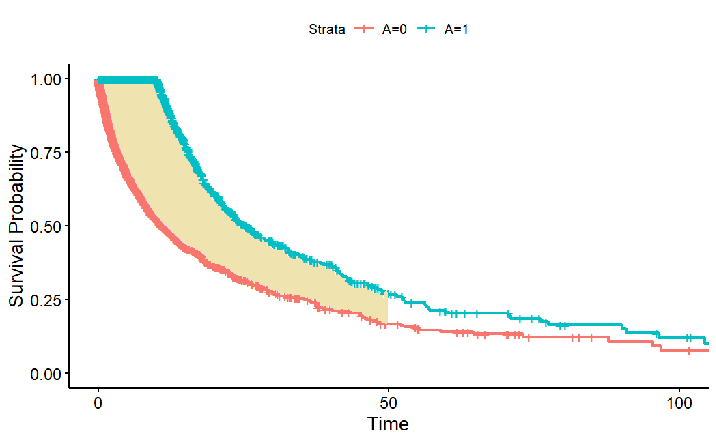
\includegraphics{KM_RMST.pdf}

}

\caption{\label{fig-RMST}Plot of the estimated survival curves on
synthetic toy-data. The \(\theta_{\mathrm{RMST}}\) at \(\tau=50\)
corresponds to the yellow shaded area between the two survival curves.
The curves have been estimated using Kaplan-Meier estimator, see
Section~\ref{sec-theoryRCT_indc}.}

\end{figure}%

Although the present work focuses on the estimation of the difference in
RMST, we would like to stress that the causal effect can be assessed
through other measures, such as for instance the difference of the
survival functions \[
\theta_{\mathrm{SP}} := S^{(1)}(\tau) - S^{(0)}(\tau) 
\] for some time \(\tau\), see for instance (Ozenne et al. 2020). As
mentionned in Section~\ref{sec-context}, another widely used measure
(though not necessarily causal) is the hazards ratio, defined as \[
\theta_{\mathrm{HR}} := \frac{\lambda^{(1)}(\tau)}{\lambda^{(0)}(\tau)},
\] where the hazard function \(\lambda^{(a)}\) is defined as \[
\lambda^{(a)}(t) := \lim_{h \to 0^+}\frac{\mathbb{P}(T(a) \in [t,t+j)|T(a) \geqslant t)}{h}.
\] in a continuous setting, or as
\(\lambda^{(a)}(t) := \mathbb{P}(T(a) = t|T(a) \geqslant t)\) when the
survival times are discrete. The hazard functions and the survival
functions are linked through the identities
\begin{equation}\phantomsection\label{eq-lambdacont}{
S^{(a)}(t) = \exp\left(-\Lambda^{(a)}(t)\right) \quad \text{where} \quad \Lambda^{(a)}(t) := \int_0^t \lambda^{(a)}(s)\mathop{}\!\mathrm{d}s,
}\end{equation} in the continuous case. The functions \(\Lambda^{(a)}\)
are call the cumulative hazard functions. In the discrete case, we have
in turn \begin{equation}\phantomsection\label{eq-lambdadisc}{
S^{(a)}(t) = \prod_{t_k \leqslant t} \left(1-\lambda^{(a)}(t_k)\right),
}\end{equation} where \(\{t_1,\dots,t_K\}\) are the atoms of
\(T^{(a)}\). These hazard functions are classically used to model the
survival times and the censoring times, see Section~\ref{sec-Gformula}.

\subsection{Organisation of the paper}\label{organisation-of-the-paper}

In this paper, we detail the minimal theoretical framework that allows
the analysis of established RMST estimators in the context of both
Randomized Controlled Trials (Section~\ref{sec-theoryRCT}) and
observational data (Section~\ref{sec-theoryOBS}). We give their
statistical properties (consistency, asymptotic normality) along with
proofs when possible. We then conduct in Section~\ref{sec-simulation} a
numerical study of these estimators through simulations under various
experimental conditions, including independent and conditionally
independent censoring and correct and incorrect model specifications. We
conclude in Section~\ref{sec-conclusion} with practical recommendations
on estimator selection, based on criteria such as asymptotic behavior,
computational complexity, and efficiency.

\subsection{Notations}\label{notations}

We provide in Table~\ref{tbl-reminder_notations} a summary of the
notation used throughout the paper.

\begin{longtable}[]{@{}
  >{\raggedright\arraybackslash}p{(\columnwidth - 2\tabcolsep) * \real{0.2083}}
  >{\raggedright\arraybackslash}p{(\columnwidth - 2\tabcolsep) * \real{0.7917}}@{}}
\caption{Summary of the
notations.}\label{tbl-reminder_notations}\tabularnewline
\toprule\noalign{}
\begin{minipage}[b]{\linewidth}\raggedright
Symbol
\end{minipage} & \begin{minipage}[b]{\linewidth}\raggedright
Description
\end{minipage} \\
\midrule\noalign{}
\endfirsthead
\toprule\noalign{}
\begin{minipage}[b]{\linewidth}\raggedright
Symbol
\end{minipage} & \begin{minipage}[b]{\linewidth}\raggedright
Description
\end{minipage} \\
\midrule\noalign{}
\endhead
\bottomrule\noalign{}
\endlastfoot
\(X\) & Covariates \\
\(A\) & Treatment indicator \((A=1\) for treatment, \(A=0\) for
control\()\) \\
\(T\) & Survival time \\
\(T(a), a \in \{0,1\}\) & Potential survival time respectively with and
without treatment \\
\(S^{(a)},a \in \{0,1\}\) & Survival function
\(S^{(a)}(t) =\mathbb{P}(T(a) > t)\) of the potential survival times \\
\(\lambda^{(a)},a \in \{0,1\}\) & Hazard function
\(\lambda^{(a)}(t) =\lim_{h \to 0^+}\mathbb{P}(T(a) \in [t,t+h) |T(a)\geqslant t)/h\)
of the potential survival times \\
\(\Lambda^{(a)},a \in \{0,1\}\) & Cumulative hazard function of the
potential survival times \\
\(C\) & Censoring time \\
\(S_C\) & Survival function \(S_C(t) =\mathbb{P}(C > t)\) of the
censoring time \\
\(G\) & Left-limit of the survival function
\(G(t) =\mathbb{P}(C \geqslant t)\) of the censoring time \\
\(\widetilde{T}\) & Observed time (\(T \wedge C\)) \\
\(\Delta\) & Censoring status \(\mathbb{I}\{T \leqslant C \}\) \\
\(\Delta^{\tau}\) & Censoring status of the restricted time
\(\Delta^{\tau} = \max\{\Delta, \mathbb{I}\{\widetilde{T} \geqslant\tau\}\}\) \\
\(\{t_{1},t_{2},\dots,t_{K}\}\) & Discrete times \\
\(e(x)\) & Propensity score \(\mathbb{E} [A| X = x]\) \\
\(\mu(x,a), a \in \{0,1\}\) &
\(\mathbb{E}[T \wedge \tau \mid X=x,A=a ]\) \\
\(S(t|x,a), a \in \{0,1\}\) & Conditional survival function,
\(\mathbb{P}(T > t | X=x, A =a)\). \\
\(\lambda^{(a)}(t|x), a \in \{0,1\}\) & Conditional hazard functions of
the potential survival times \\
\(G(t|x,a), a \in \{0,1\}\) & left-limit of the conditional survival
function of the censoring \(\mathbb{P}(C\geqslant t|X=x,A=a)\) \\
\(Q_{S}(t|x,a), a \in \{0,1\}\) &
\(\mathbb{E}[T \wedge \tau \mid X=x,A=a, T \wedge \tau>t]\) \\
\end{longtable}

\section{Causal survival analysis in Randomized Controlled
Trials}\label{sec-theoryRCT}

Randomized Controlled Trials (RCTs) are the gold standard for
establishing the effect of a treatment on an outcome, because treatment
allocation is controlled through randomization, which ensures
(asymptotically) the balance of covariates between treated and controls,
and thus avoids problems of confounding between treatment groups. The
core assumption in a classical RCT is the random assignment of the
treatment (D. B. Rubin 1974).

\textbf{Assumption.} (Random treatment assignment) There holds:
\begin{equation}\phantomsection\label{eq-rta}{ 
A \perp\mkern-9.5mu\perp T(0),T(1),X
}\end{equation}

We also assume that there is a positive probability of receiving the
treatment, which we rephrase under the following assumption.

\textbf{Assumption.} (Trial positivity)
\begin{equation}\phantomsection\label{eq-postrial}{ 
0 < \mathbb{P}(A=1) < 1
}\end{equation}

Under Assumptions \ref{eq-rta} and \ref{eq-postrial}, classical causal
identifiability equations can be written to express
\(\theta_{\mathrm{RMST}}\) without potential outcomes.

\begin{equation}\phantomsection\label{eq-RMSTkm}{
\begin{aligned}
    \theta_{\mathrm{RMST}} &=  \mathbb{E}[T(1) \wedge \tau - T(0) \wedge \tau]\\
    &= \mathbb{E}[T(1) \wedge \tau | A = 1] - \mathbb{E}[ T(0) \wedge \tau| A= 0]  && \tiny\text{(Random treatment assignment)} \\
       &= \mathbb{E}[T \wedge \tau | A = 1] - \mathbb{E}[ T \wedge \tau| A= 0].  && \tiny\text{(SUTVA)}
\end{aligned}
}\end{equation}

However, Equation~\ref{eq-RMSTkm} still depends on \(T\), which remains
only partially observed due to censoring. To ensure that censoring does
not compromise the identifiability of treatment effects, we must impose
certain assumptions on the censoring process, standards in survival
analysis, namely, independent censoring and conditionally independent
censoring. These assumptions lead to different estimation approaches. We
focus on two strategies: those that aim to directly estimate
\(\mathbb{E}[T \wedge \tau | A = a]\) directly (e.g., through
censoring-unbiased transformations, see Section~\ref{sec-condcens}), and
those that first estimate the survival curves to derive RMST via
Equation~\ref{eq-rmstsurv} (such as the Kaplan-Meier estimator and all
its variants, see the next Section).

\subsection{Independent censoring: the Kaplan-Meier
estimator}\label{sec-theoryRCT_indc}

In a first approach, one might assume that the censoring times are
independent from the rest of the variables.

\textbf{Assumption.} (Independent censoring)
\begin{equation}\phantomsection\label{eq-independantcensoring}{ 
C \perp\mkern-9.5mu\perp T(0),T(1),X,A.
}\end{equation}

Under Equation~\ref{eq-independantcensoring}, subjects censored at time
\(t\) are representative of all subjects who remain at risk at time
\(t\). Figure~\ref{fig-RCT_ind_causalgraph} represents the causal graph
when the study is randomized and outcomes are observed under independent
censoring.

\begin{figure}

\centering{

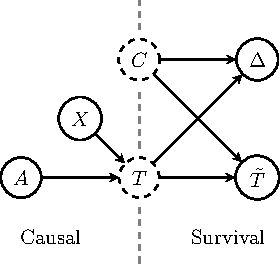
\includegraphics[width=0.4\textwidth,height=\textheight]{causal_survival_rct_indep.pdf}

}

\caption{\label{fig-RCT_ind_causalgraph}Causal graph in RCT survival
data with independent censoring.}

\end{figure}%

We also assume that there is no almost-sure upper bound on the censoring
time before \(\tau\), which we rephrase under the following assumption.

\textbf{Assumption.} (Positivity of the censoring process) There exists
\(\varepsilon> 0\) such that
\begin{equation}\phantomsection\label{eq-poscen}{ 
G(t) \geqslant\varepsilon\quad \text{for all} \quad t \in [0,\tau).
}\end{equation}

If indeed it was the case that \(\mathbb{P}(C < t) = 1\) for some
\(t < \tau\), then we would not be able to infer anything on the
survival function on the interval \([t,\tau]\) as all observation times
\(\widetilde T_i\) would be in \([0,t]\) almost surely. In practice,
adjusting the threshold time \(\tau\) can help satisfy the positivity
assumption. For instance, in a clinical study, if a subgroup of patients
has zero probability of remaining uncensored at a given time, \(\tau\)
can be modified to ensure that participants have a feasible chance of
remaining uncensored up to the revised threshold.

The two Assumptions \ref{eq-independantcensoring} and \ref{eq-poscen}
together allow the distributions of \(T(a)\) to be identifiable, in the
sense that there exists an identity that expresses \(S^{(a)}\) as a
function of the joint distribution of \((\widetilde T,\Delta,A=a)\), see
for instance Ebrahimi, Molefe, and Ying (2003) for such a formula in a
non-causal framework. This enables several estimation strategies, the
most well-known being the Kaplan-Meier product-limit estimator.

To motivate the definition of the latter and explicit the
identifiability identity, we set the analysis in the discrete case. We
let \(\{t_k\}_{k \geqslant 1}\) be a set of positive and increasing
times and assume that \(T \in \{t_k\}_{k \geqslant 1}\) almost surely.
Then for any \(t \in [0,\tau]\), it holds, letting \(t_0 = 0\) by
convention, thanks to Equation~\ref{eq-lambdadisc},

\begin{align*}
S(t| A=a) &= \mathbb{P}(T > t|A=a) = \prod_{t_k \leqslant t} \left(1 - \mathbb{P}(T = t_k | T > t_{k-1}, A=a)\right) \\
&= \prod_{t_k \leqslant t} \left(1 - \frac{\mathbb{P}(T = t_{k}, A=a)}{\mathbb{P}(T \geqslant t_{k},A=a)}\right).
\end{align*}

Using Assumptions \ref{eq-independantcensoring} and \ref{eq-poscen}, we
find that \begin{equation}\phantomsection\label{eq-kmindep}{
\frac{\mathbb{P}(T = t_{k}, A=a)}{\mathbb{P}(T \geqslant t_{k},A=a)} = \frac{\mathbb{P}(T = t_{k},C \geqslant t_k,A=a)}{\mathbb{P}(T \geqslant t_{k}, C\geqslant t_k,A=a)} =  \frac{\mathbb{P}(\widetilde T = t_{k}, \Delta = 1,A=a)}{\mathbb{P}( \widetilde T \geqslant t_{k},A=a)},
}\end{equation} yielding the final identity
\begin{equation}\phantomsection\label{eq-kmi}{ 
S(t|A=a) = \prod_{t_k \leqslant t} \left(1-\frac{\mathbb{P}(\widetilde T = t_{k}, \Delta = 1,A=a)}{\mathbb{P}( \widetilde T \geqslant t_{k},A=a)}\right).
}\end{equation} Notice that the right hand side only depends on the
distribution of the observed tuple \((A,\widetilde T,\Delta)\). This
last equation suggests in turn to introduce the quantities
\begin{equation}\phantomsection\label{eq-dknk}{
D_k(a) := \sum_{i=1}^n \mathbb{I}(\widetilde T_i = t_k, \Delta_i = 1, A=a) \quad\text{and}\quad N_k(a) := \sum_{i=1}^n \mathbb{I}(\widetilde T_i \geqslant t_k, A=a),
}\end{equation} which correspond respectively to the number of deaths
\(D_k(a)\) and of individuals at risk \(N_k(a)\) at time \(t_k\) in the
treated group (a=1) or in the control group (a=0).

\begin{definition}[]\protect\hypertarget{def-km}{}\label{def-km}

(Kaplan-Meier estimator, Kaplan and Meier (1958)) With \(D_k(a)\) and
\(N_k(a)\) defined in Equation~\ref{eq-dknk}, we let

\begin{equation}\phantomsection\label{eq-unadjKM}{
    \widehat{S}_{\mathrm{KM}}(t|A=a) := \prod_{t_k \leqslant t}\left(1-\frac{D_k(a)}{N_k(a)}\right).
}\end{equation}

\end{definition}

The assiociated RMST estimator is then simply defined as
\begin{equation}\phantomsection\label{eq-thetaunadjKM}{
\widehat{\theta}_{\mathrm{KM}} = \int_{0}^{\tau}\widehat{S}_{KM}(t|A=1)-\widehat{S}_{KM}(t|A=0)dt.
}\end{equation} The Kaplan-Meier estimator is the Maximum Likelihood
Estimator (MLE) of the survival functions, see for instance Kaplan and
Meier (1958). Furthermore, because \(D_k(a)\) and \(N_k(a)\) are sums of
i.i.d. random variables, the Kaplan-Meier estimator inherits some
convenient statistical properties.

\begin{proposition}[]\protect\hypertarget{prp-km}{}\label{prp-km}

Under Assumptions
\ref{eq-sutva}, \ref{eq-rta}, \ref{eq-postrial}, \ref{eq-independantcensoring}
and \ref{eq-poscen}, and for all \(t \in [0,\tau]\), the estimator
\(\widehat S_{\mathrm{KM}}(t|A=a)\) of \(S^{(a)}(t)\) is strongly
consistent and admits the following bounds for its bias: \[
0 \leqslant S^{(a)}(t) - \mathbb{E}[\widehat S_\mathrm{KM}(t|A=a)] \leqslant O(\mathbb{P}(N_k(a) = 0)),
\] where \(k\) is the greatest time \(t_k\) such that
\(t \geqslant t_k\).

\end{proposition}

Gill (1983) gives a more precise lower-bound on the bias in the case of
continuous distributions, which was subsequently refined by Zhou (1988).
The bound we give, although slightly looser, still exhibits the same
asymptotic regime. In particular, as soon as \(S^{(a)}(t) > 0\) (and
Assumption \ref{eq-poscen} holds), then the bias decays exponentially
fast towards \(0\). We give in Section~\ref{sec-proof21} a simple proof
of our bound is our context.

\begin{proposition}[]\protect\hypertarget{prp-varkm}{}\label{prp-varkm}

Under Assumptions
\ref{eq-sutva}, \ref{eq-rta}, \ref{eq-postrial}, \ref{eq-independantcensoring}
and \ref{eq-poscen}, and for all \(t \in [0,\tau]\),
\(\widehat S_{\mathrm{KM}}(t|A=a)\) is asymptotically normal and
\(\sqrt{n}\left(\widehat S_{\mathrm{KM}}(t|A=a) - S^{(a)}(t)\right)\)
converges in distribution towards a centered Gaussian of variance \[
V_{\mathrm{KM}}(t|A=a) := S^{(a)}(t)^2 \sum_{t_k \leqslant t} \frac{1-s_k(a)}{s_k(a) r_k(a)},
\] where \(s_k(a) = S^{(a)}(t_k)/S^{(a)}(t_{k-1})\) and
\(r_k(a) = \mathbb{P}(\widetilde T \geqslant t_k, A=a)\).

\end{proposition}

The proof of Proposition~\ref{prp-varkm} can be found in
Section~\ref{sec-proof21}. Because \(D_k(a)/N_k(a)\) is a natural
estimator of \(1-s_k(a)\) and, \(\frac{1}{n} N_k(a)\) a natural
estimator for \(r_k(a)\), the asymptotic variance of the Kaplan-Meier
estimator can be estimated with the so-called Greenwood formula, as
already derived heuristically in Kaplan and Meier (1958):

\begin{equation}\phantomsection\label{eq-varkm}{
\widehat{\mathrm{Var}} \left(\widehat{S}_{\mathrm{KM}}(t|A=a)\right) := \widehat{S}_{\mathrm{KM}}(t|A=a)^2 \sum_{t_k \leqslant t} \frac{D_k(a)}{N_k(a)(N_k(a)-D_k(a))}.
}\end{equation}

We finally mention that the KM estimator as defined in
Definition~\ref{def-km} still makes sense in a non-discrete setting, and
one only needs to replace the fixed grid \(\{t_k\}\) by the values at
which we observed an event \((\widetilde T_i = t_k, \Delta_i =1)\). We
refer to Breslow and Crowley (1974) for a study of this estimator in the
continuous case and to Aalen, Borgan, and Gjessing (2008), Sec 3.2 for a
general study of the KM estimator through the prism of point processes.

\subsection{Conditionally independent censoring}\label{sec-condcens}

An alternative hypothesis in survival analysis that relaxes the
assumption of independent censoring is conditionally independent
censoring, also refered sometimes as \emph{informative censoring}. It
allows to model more realistic censoring processes, in particular in
situations where there are reasons to believe that \(C\) may be
dependent from \(A\) and \(X\) (for instance, if patient is more like to
leave the study when treated because of side-effects of the treatment).

\textbf{Assumption.} (Conditionally independent censoring)
\begin{equation}\phantomsection\label{eq-condindepcensoring}{ 
C \perp\mkern-9.5mu\perp T(0),T(1) ~ | ~X,A
}\end{equation}

Under Equation~\ref{eq-condindepcensoring}, subjects within a same
stratum defined by \(X=x\) and \(A=a\) have equal probability of
censoring at time \(t\), for all \(t\). In case of conditionally
independent censoring, we also need to assume that all subjects have a
positive probability to remain uncensored at their time-to-event.

\textbf{Assumption.} (Positivity / Overlap for censoring) There exists
\(\varepsilon> 0\) such that for all \(t\in [0,\tau)\), it almost surely
holds \begin{equation}\phantomsection\label{eq-positivitycensoring}{ 
G(t|A,X) \geqslant\varepsilon.
}\end{equation}

Figure~\ref{fig-RCT_dep_causalgraph} represents the causal graph when
the study is randomized with conditionally independent censoring.

\begin{figure}

\centering{

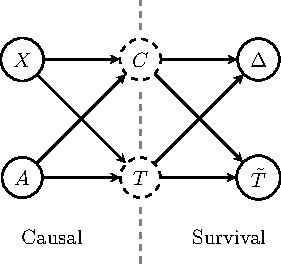
\includegraphics[width=0.4\textwidth,height=\textheight]{causal_survival_rct_dep.pdf}

}

\caption{\label{fig-RCT_dep_causalgraph}Causal graph in RCT survival
data with dependent censoring.}

\end{figure}%

Under dependent censoring, the Kaplan-Meier estimator as defined in
Definition~\ref{def-km} can fail to estimate survival, in particular
because Equation~\ref{eq-kmindep} does not hold anymore. Alternatives
include plug-in G-formula estimators (Section~\ref{sec-Gformula}) and
unbiased transformations (Section~\ref{sec-unbiasedtransfo}).

\subsubsection{The G-formula and the Cox Model}\label{sec-Gformula}

Because the censoring is now independent from the potential outcome
conditionally to the covariates, it would seem natural to model the
response of the survival time conditionally to these covariates too: \[
\mu(x,a) := \mathbb{E}[T \wedge \tau |X = x, A = a].
\]

Building on Equation~\ref{eq-RMSTkm}, one can express the RMST as a
function of \(\mu\): \begin{align*}
 \theta_{\mathrm{RMST}} = \mathbb{E}\left[\mathbb{E}[T \wedge \tau |X, A = 1]\right] - \mathbb{E}\left[ T \wedge \tau|X, A= 0]\right] = \mathbb{E}[\mu(X,1)-\mu(X,0)].
\end{align*}

An estimator \(\widehat\mu\) of \(\mu\) would then straightforwardly
yield an estimator of the difference in RMST through the so-called
\emph{G-formula} plug-in estimator:

\begin{equation}\phantomsection\label{eq-gformula}{ \widehat{\theta}_{\mathrm{G-formula}} = \frac{1}{n} \sum_{i=1}^n \widehat\mu\left(X_i, 1\right)-\widehat\mu\left(X_i, 0\right). }\end{equation}

We would like to stress that a G-formula approach works also in a
observational context as the one introduced in
Section~\ref{sec-obscondcens}. However, because the estimation
strategies presented in the next sections relies on estimating nuisance
parameters, and that this latter task is often done in the same way as
we estimate the conditional response \(\mu\), we decided to not delay
the introduction of the G-formula any further, and we present below a
few estimation methods for \(\mu\). These methods are sub-divised in two
categories: \emph{\(T\)-learners}, where \(\mu(\cdot,1)\) is estimated
separately from \(\mu(\cdot,0)\), and \_\(S\)-learners, where
\(\widehat\mu\) is obtained by fitting a single model based on
covariates \((X,A)\).

\textbf{Cox's Model}. There are many ways to model \(\mu\) in a survival
context, the most notorious of which being the Cox proportional hazards
model (Cox 1972). It relies on a semi-parametric modelling the
conditional hazard functions \(\lambda^{(a)}(t|X)\) as \[
\lambda^{(a)}(t|X) = \lambda_0^{(a)}(t) \exp(X^\top\beta^{(a)}),
\] where \(\lambda^{(a)}_0\) is a baseline hazard function and
\(\beta^{(a)}\) has the same dimension as the vector of covariate \(X\).
The conditional survival function then take the simple form (in the
continuous case) \[
S^{(a)}(t|X) = S^{(a)}_0(t)^{\exp(X^\top\beta^{(a)})},
\] where \(S^{(a)}_0(t)\) is the survival function associated with
\(\lambda_0^{(a)}\). The vector \(\beta^{(a)}\) is classically estimated
by maximizing the so-called \emph{partial likelihood} function as
introduced in the original paper of Cox (1972): \[
\mathcal{L}(\beta) := \prod_{\Delta_i = 1} \frac{\exp(X_i^\top \beta)}{\displaystyle\sum_{\widetilde T_j \geqslant\widetilde T_i} \exp(X_j^\top \beta)},
\]

while the cumulative baseline hazard function can be estimated through
the Breslow's estimator (Breslow 1974): \[
\widehat\Lambda_0^{(a)}(t) = \sum_{\Delta_i = 1, \widetilde T_i \leqslant t} \frac{1}{\displaystyle\sum_{\widetilde T_j \geqslant\widetilde T_i} \exp(X_j^\top \widehat\beta^{(a)})} 
\] where \(\widehat\beta^{(a)}\) is a partial likelihood maximizer. One
can show that \((\widehat\beta^{(a)},\widehat\Lambda_0^{(a)})\) is the
MLE of the true likelihood, when \(\widehat\Lambda_0^{(a)}\) is
optimized over all step fonctions of the form \[
\Lambda_0(t) := \sum_{\Delta_i=1} h_i, \quad h_i \in \mathbb{R}^+.
\] This fact was already hinted in the original paper by Cox and made
rigorous in many subsequent papers, see for instance Fan, Feng, and Wu
(2010). Furthermore, if the true distribution follows a Cox model, then
both \(\widehat\beta^{(a)}\) and \(\widehat\Lambda_0^{(a)}\) are
strongly consistent and asymptotically normal estimator of the true
parameters \(\beta^{(a)}\) and \(\Lambda^{(a)}\), see Kalbfleisch and
Prentice (2002), Sec 5.7. When using a \(T\)-learner approach, one
simply finds \((\widehat\beta^{(a)},\widehat\Lambda_0^{(a)})\) for
\(a \in \{0,1\}\) by considering the control group and the treated group
separately. When using a \(S\)-learner approach, the treatment status
\(A\) becomes a covariate a the model becomes
\begin{equation}\phantomsection\label{eq-coxslearner}{
\lambda(t|X,A) = \lambda_0(t) \exp(X^\top\beta+\alpha A).
}\end{equation} for some \(\alpha \in \mathbb{R}\). One main advantage
of Cox's model is that it makes it very easy to interpret the effect of
a covariate on the survival time. If indeed \(\alpha > 0\), then the
treatment has a negative effect of the survival times. Likewise, if
\(\beta_i >0\), then the \(i\)-th coordinate of \(X\) has a negative
effect as well. We finally mention that the hazard ratio takes a
particularly simple form under the later model since \[
\theta_{\mathrm{HR}} = e^{\alpha}.
\] In particular, it does not depends on the time horizon \(\tau\), and
is thus sometimes refered to as \emph{proportional hazard}.
Figure~\ref{fig-gf} illustrates the estimation of the difference in
Restricted Mean Survival Time using G-formula with Cox models.

\begin{figure}

\centering{

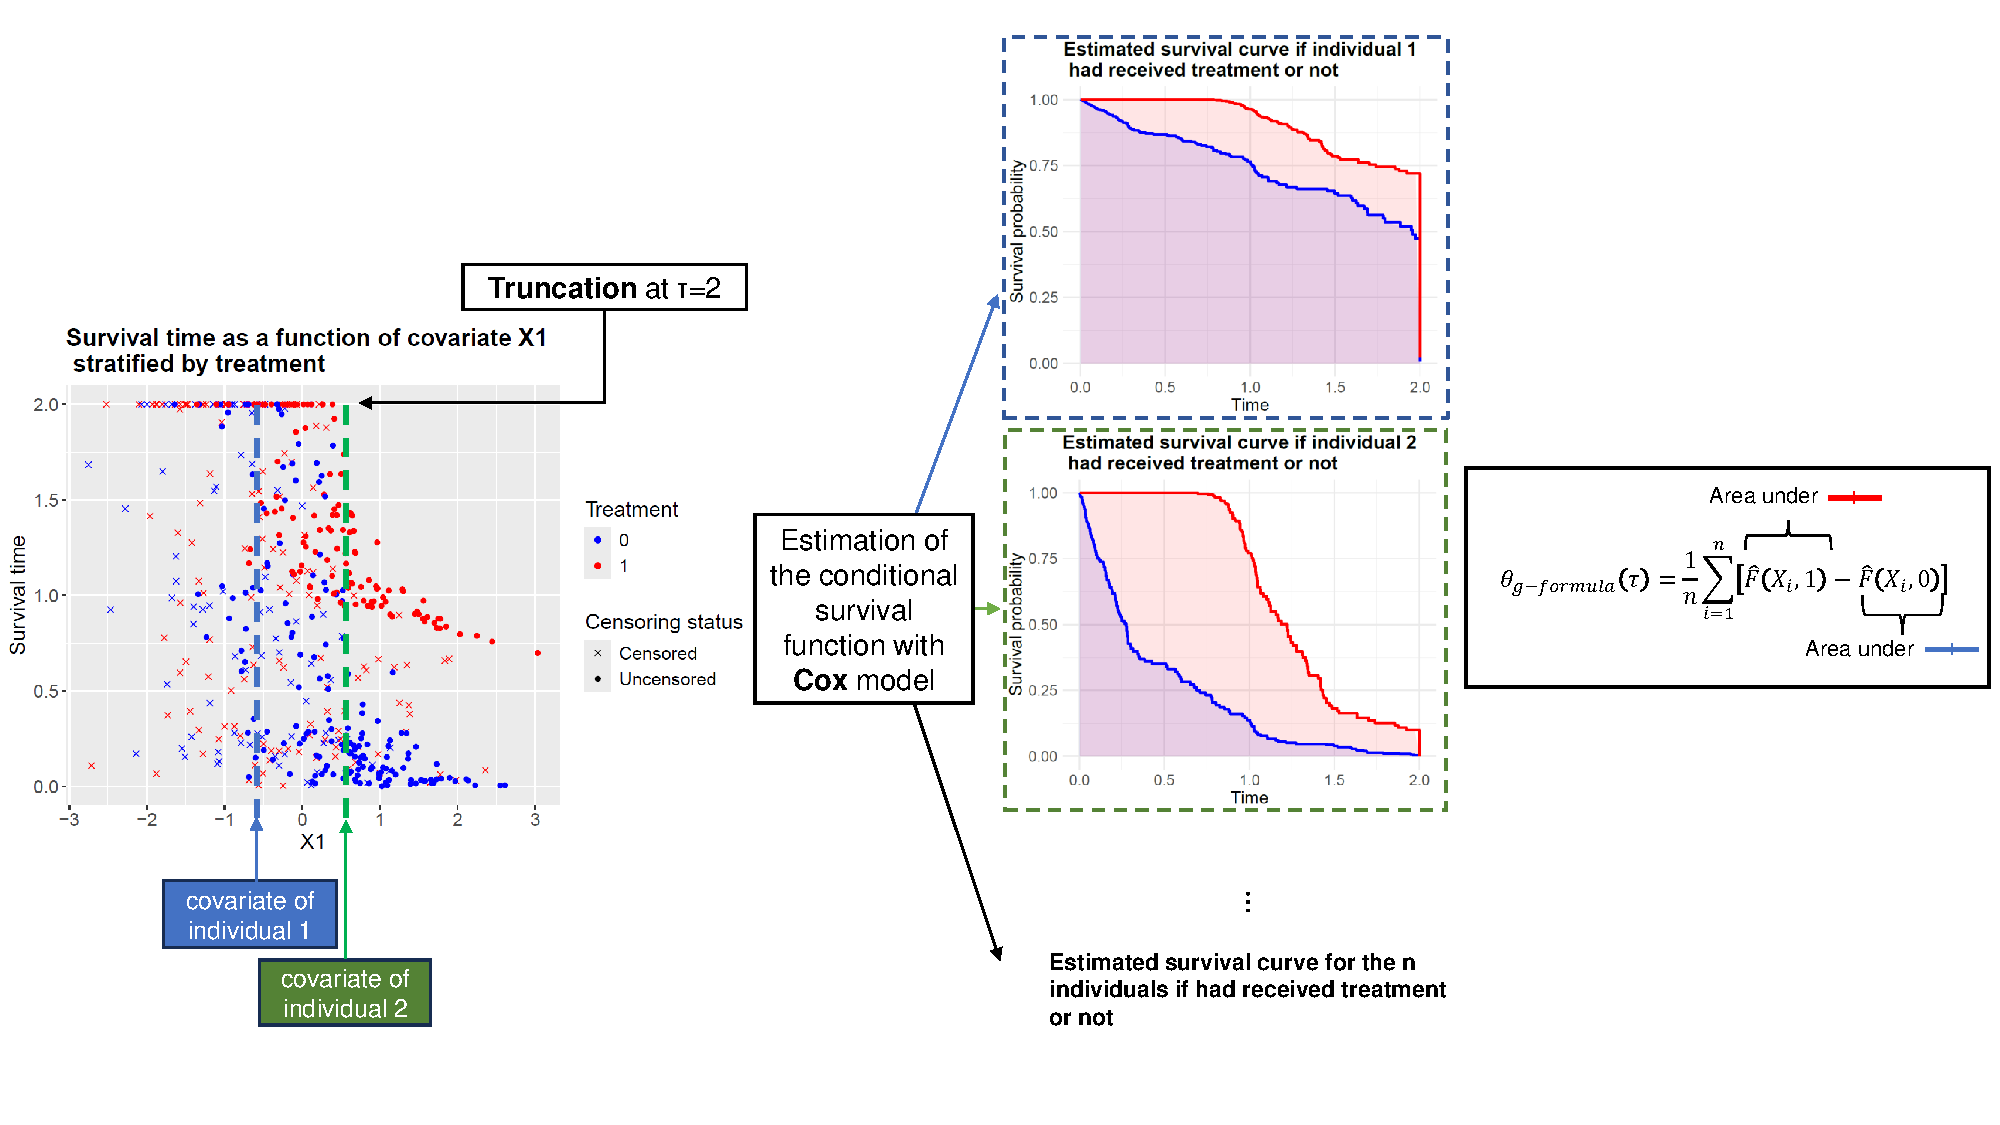
\includegraphics[width=1.1\textwidth,height=\textheight]{G_formula_RCT.pdf}

}

\caption{\label{fig-gf}Illustration of the G-formula for estimating
\(\theta_{\mathrm{RMST}}\) in an RCT when only one covariate \(X_1\)
influences the outcome.}

\end{figure}%

\textbf{Weibull Model}. A popular parametric model for survival is the
Weibull Model, which amounts to assume that \[
\lambda^{(a)}(t|X) = \lambda_0^{(a)}(t) \exp(X^\top\beta)
\] where \(\lambda_0^{(a)}(t)\) is the instant hazard function of a
Weibull distribution, that is to say a function proportional to
\(t^{\gamma}\) for some shape parameter \(\gamma >0\). We refer to Zhang
(2016) for a study of this model.

\textbf{Survival Forests}. On the non-parametric front, we mention the
existence of survival forests (Ishwaran et al. 2008).

\subsubsection{Censoring unbiased
transformations}\label{sec-unbiasedtransfo}

Censoring unbiased transformations involve applying a transformation to
\(T\). Specifically, we compute a new time \(T^*\) of the form
\begin{equation}\phantomsection\label{eq-defcut}{
T^* := T^*(\widetilde T,X,A,\Delta) = \begin{cases}
\phi_0(\widetilde T \wedge \tau,X,A) \quad &\text{if} \quad \Delta^\tau = 0, \\
\phi_1(\widetilde T \wedge \tau,X,A) \quad &\text{if} \quad \Delta^\tau = 1.
\end{cases}
}\end{equation} for two wisely chosen transformations \(\phi_0\) and
\(\phi_1\), and where
\begin{equation}\phantomsection\label{eq-defdeltatau}{\Delta^{\tau}:=\mathbb{I}\{T \wedge \tau \leqslant C\} = \Delta+(1-\Delta)\mathbb{I}(\widetilde T \geqslant\tau)
}\end{equation} is the indicator of the event where the individual is
either uncensored or censored after time \(\tau\). The idea behind the
introduction of \(\Delta^\tau\) is that because we are only interested
in computed the expectation of the survival time thresholded by
\(\tau\), any censored observation coming after time \(\tau\) can in
fact be considered as uncensored (\(\Delta^\tau = 1\)).

A censoring unbiased transformation \(T^*\) shall satisfy: for
\(a \in \{0,1\}\), it holds
\begin{equation}\phantomsection\label{eq-cut}{
\mathbb{E}[T^*|A=a,X] = \mathbb{E}[T(a) \wedge \tau |X] \quad\text{almost surely.}
}\end{equation} A notable advantage of this approach is that it enables
the use of the full transformed dataset \((X_i,A_i,T^*_i)\) as if no
censoring occured. Because it holds
\begin{equation}\phantomsection\label{eq-cutcond}{
\mathbb{E}[\mathbb{E}[T^*|A=a,X]] = \mathbb{E}\left[\frac{\mathbb{I}\{A=a\}}{\mathbb{P}(A=a)} T^*\right],
}\end{equation} there is a very natural way to derive an estimator of
the difference in RMST from any censoring unbiased transformation
\(T^*\) as: \begin{equation}\phantomsection\label{eq-cutest}{
\widehat\theta = \frac1n\sum_{i=1}^n \left(\frac{A_i}{\pi}-\frac{1-A_i}{1-\pi} \right) T^*_i
}\end{equation} where \(\pi = \mathbb{P}(A=1) \in (0,1)\) by Assumption
\ref{eq-postrial} and where
\(T^*_i = T^*(\widetilde T_i,X_i,A_i,\Delta_i)\). We easily get the
following result.

\begin{proposition}[]\protect\hypertarget{prp-cutest}{}\label{prp-cutest}

Under Assumptions \ref{eq-rta} and \ref{eq-postrial}, the estimator
\(\widehat\theta\) derived as in Equation~\ref{eq-cutest} from a square
integrable censoring unbiased transformations satisfying
Equation~\ref{eq-cut} is an unbiased, strongly consistent, and
asymptotically normal estimator of the difference in RMST.

\end{proposition}

Square integrability will be ensured any time the transformnation is
bounded, which will always be the case of the ones considered in this
work. It is natural in a RCT setting to assume that probability of being
treated \(\pi\) is known. If not, it is usual to replace \(\pi\) by its
empirical counterpart \(\widehat\pi = n_1/n\) where
\(n_a = \sum_{i} \mathbb{1}\{A=a\}\). The resulting estimator takes the
form \begin{equation}\phantomsection\label{eq-cutestnopi}{
\widehat\theta = \frac1{n_1}\sum_{A_i = 1}  T^*_i - \frac1{n_0}\sum_{A_i = 0}  T^*_i.
}\end{equation} Note however that this estimator is slighlty biased due
to the estimation of \(\pi\) (see for instance Colnet et al. (2022),
Lemma 2), but it is still strongly consistent and asymptotically normal,
and its biased is exponentially small in \(n\).

\begin{proposition}[]\protect\hypertarget{prp-cutestnopi}{}\label{prp-cutestnopi}

Under Assumptions \ref{eq-rta} and \ref{eq-postrial}, the estimator
\(\widehat\theta\) derived as in Equation~\ref{eq-cutestnopi} from a
square integrable censoring unbiased transformations satisfying
Equation~\ref{eq-cut} is a strongly consistent, and asymptotically
normal estimator of the difference in RMST.

\end{proposition}

The two most popular transformations are
Inverse-Probability-of-Censoring Weighting (Koul, Susarla, and Ryzin
(1981)) and Buckley-James (Buckley and James (1979)), both illustrated
in Figure~\ref{fig-trans} and detailed below. In the former, only
non-censored observations are considered and they are weighted while in
the latter, censored observations are imputed with an estimated survival
time.

\begin{figure}

\centering{

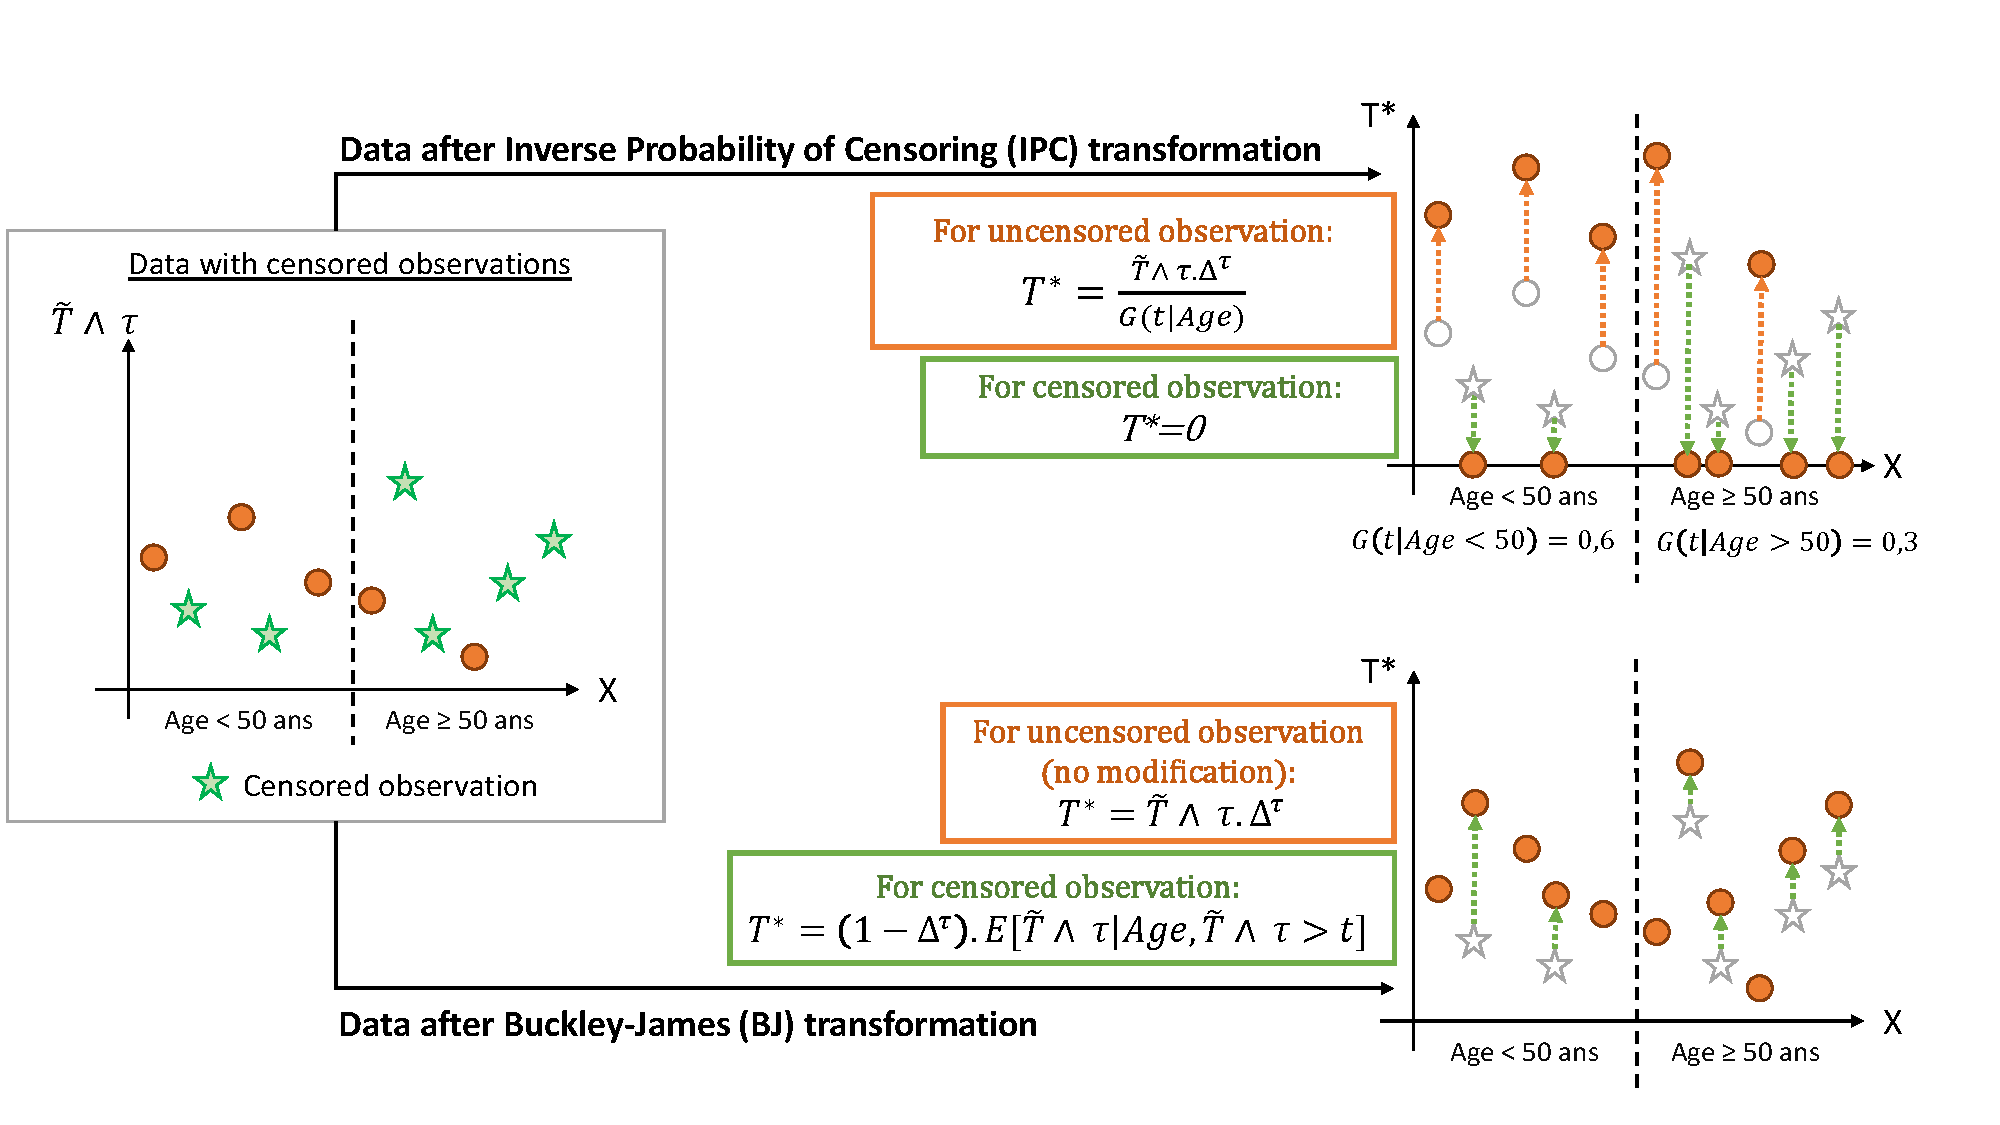
\includegraphics{schema_transformation.pdf}

}

\caption{\label{fig-trans}Illustration of
Inverse-Probability-of-Censoring and Buckley-James transformations.}

\end{figure}%

\textbf{The Inverse-Probability-of-Censoring Weighted transformation}

The Inverse-Probability-of-Censoring Weighted (IPCW) transformation,
introduced by (Koul, Susarla, and Ryzin (1981)) in the context of
censored linear regression, involves discarding censored observations
and applying weights to uncensored data. More precisely, we let
\begin{equation}\phantomsection\label{eq-defipcw}{
T^*_{\mathrm{IPCW}}=\frac{\Delta^\tau}{G(\widetilde{T}\wedge \tau|X,A)} \widetilde{T} \wedge \tau,
}\end{equation} where we recall that
\(G(t|X,A) :=\mathbb{P}(C \geqslant t|X,A)\) is the left limit of the
conditional survival function of the censoring. This estimator assigns
higher weights to uncensored subjects within a covariate group that is
highly prone to censoring, thereby correcting for conditionally
independent censoring and reducing selection bias (Howe et al. 2016).

\begin{proposition}[]\protect\hypertarget{prp-ipcw}{}\label{prp-ipcw}

Under Assumptions
\ref{eq-sutva}, \ref{eq-rta}, \ref{eq-postrial}, \ref{eq-condindepcensoring}
and \ref{eq-positivitycensoring}, the IPCW transform \ref{eq-defipcw} is
a censoring unbiased transformation in the sense of
Equation~\ref{eq-cut}.

\end{proposition}

The proof of Proposition~\ref{prp-ipcw} is in Section~\ref{sec-proof22}.
The IPCW depends on the unknown conditional survival function of the
censoring \(G(\cdot|X,A)\), which thus needs to be estimated. Estimating
conditional censoring or the conditional survival function can be
approached similarly, as both involve estimating a time---whether for
survival or censoring. Consequently, we can use semi-parametric methods,
such as the Cox model, or non-parametric approaches like survival
forests, and we refer to Section~\ref{sec-Gformula} for a development on
these approaches. Once an estimator \(\widehat G(\cdot|A,X)\) of the
later is provided, one can construct an estimator of the difference in
RMST based on Equation~\ref{eq-cutest} or Equation~\ref{eq-cutestnopi}
\begin{equation}\phantomsection\label{eq-ipcwdef}{
\widehat\theta_{\mathrm{IPCW}} = \frac1n \sum_{i=1}^n \left(\frac{A_i}{\pi}-\frac{1-A_i}{1-\pi}\right) T^*_{\mathrm{IPCW},i}, 
}\end{equation} or
\begin{equation}\phantomsection\label{eq-ipcwdefnopi}{
\widehat\theta_{\mathrm{IPCW}} = \frac1{n_1}\sum_{A_i = 1}  T^*_{\mathrm{IPCW},i} - \frac1{n_0}\sum_{A_i = 0}  T^*_{\mathrm{IPCW},i}. 
}\end{equation} where we recall that \(n_a := \#\{i \in [n]~|~A_i=a\}\).
By Proposition~\ref{prp-cutest}, Proposition~\ref{prp-cutestnopi} and
Proposition~\ref{prp-ipcw}, we easily deduce that
\(\widehat\theta_{\mathrm{IPCW}}\) is asymptotically consistent as soon
as \(\widehat G\) is.

\begin{corollary}[]\protect\hypertarget{cor-ipcwcons}{}\label{cor-ipcwcons}

Under
Assumptions\ref{eq-sutva}, \ref{eq-rta}, \ref{eq-postrial}, \ref{eq-condindepcensoring}
and \ref{eq-positivitycensoring}, if \(\widehat G\) is uniformly weakly
(resp. strongly) consistent then so is
\(\widehat\theta_{\mathrm{IPCW}}\), either as in defined in
Equation~\ref{eq-ipcwdef} or in Equation~\ref{eq-ipcwdefnopi}.

\end{corollary}

This result simply comes from the fact that
\(\widehat\theta_{\mathrm{IPCW}}\) depends continuously on
\(\widehat G\) and that \(G\) is lower-bounded (Assumption
\ref{eq-positivitycensoring}). Surprisingly, we found limited use of
this estimator in the literature, beside its first introduction in Koul,
Susarla, and Ryzin (1981). This could potentially be explained by the
fact that, empirically, we observed that this estimator is highly
variable. Consequently, we do not explore its properties further and
will not include it in the numerical experiments. A related and more
popular estimator is the IPCW-Kaplan-Meier, defined as follows.

\begin{definition}[]\protect\hypertarget{def-ipcwkm}{}\label{def-ipcwkm}

(IPCW-Kaplan-Meier) We let again \(\widehat G(\cdot|X,A)\) be an
estimator of the (left limit of) the conditional censoring survival
function and we introduce

\begin{align*}
D_k^{\mathrm{IPCW}}(a) &:= \sum_{i=1}^n \frac{\Delta_i^\tau}{\widehat G(\widetilde T_i \wedge\tau | X_i,A=a)} \mathbb{I}(\widetilde T_i = t_k, A_i=a) \\
\quad\text{and}\quad N^{\mathrm{IPCW}}_k(a) &:= \sum_{i=1}^n \frac{\Delta_i^\tau}{\widehat G(\widetilde T_i \wedge\tau | X_i,A=a)} \mathbb{I}(\widetilde T_i \geqslant t_k, A_i=a),
\end{align*}

be the weight-corrected numbers of deaths and of individual at risk at
time \(t_k\). The IPCW version of the KM estimator is then defined as:
\[
\begin{aligned}
\widehat{S}_{\mathrm{IPCW}}(t | A=a) &= \prod_{t_k \leqslant t}\left(1-\frac{D_k^{\mathrm{IPCW}}(a)}{N_k^{\mathrm{IPCW}}(a)}\right). 
\end{aligned}
\]

\end{definition}

Note that the quantity \(\pi\) is not present in the definition of
\(D_k^{\mathrm{IPCW}}(a)\) and \(N_k^{\mathrm{IPCW}}(a)\) because it
would simply disappear in the ratio
\(D_k^{\mathrm{IPCW}}(a)/N_k^{\mathrm{IPCW}}(a)\). The subsequent RMST
estimator then take the form
\begin{equation}\phantomsection\label{eq-thetaIPCWKM}{
\widehat{\theta}_{\mathrm{IPCW-KM}} = \int_{0}^{\tau}\widehat{S}_{\mathrm{IPCW}}(t|A=1)-\widehat{S}_{\mathrm{IPCW}}(t|A=0)dt.
}\end{equation} Like before for the classical KM estimator, this new
reweighted KM estimator enjoys good statistical properties.

\begin{proposition}[]\protect\hypertarget{prp-ipcwkm}{}\label{prp-ipcwkm}

Under Assumptions
\ref{eq-sutva}, \ref{eq-rta}, \ref{eq-postrial}, \ref{eq-condindepcensoring}
and \ref{eq-positivitycensoring}, and for all \(t \in [0,\tau]\), the
oracle estimator \(S^*_{\mathrm{IPCW}}(t|A=a)\) defined as in
Definition~\ref{def-ipcwkm} with \(\widehat G = G\) is a stronlgy
consistent and asymptotically normal estimator of \(S^{(a)}(t)\) .

\end{proposition}

The proof of Proposition~\ref{prp-ipcwkm} can be found in
Section~\ref{sec-proof22}. Because the evaluation of
\(N_k^{\textrm{IPCW}}(a)\) now depends on information gathered after
time \(t_k\) (through the computation of the weights), the previous
proofs on the absence of bias and on the derivation of the asymptotic
variance unfortunately do not carry over in this case. Whether its bias
is exponentially small and whether the asymptotic variance can be
derived in a closed form are questions left open. We are also not aware
of any estimation schemes for the asymptotic variance in this context.
In the case where we do not have access to the oracle survival function
\(G\), we can again still achieve consistency if the estimator
\(\widehat G(\cdot|A,X)\) that we provide is consistent.

\begin{corollary}[]\protect\hypertarget{cor-ipcwkmcons}{}\label{cor-ipcwkmcons}

Under Assumptions
\ref{eq-sutva}, \ref{eq-rta}, \ref{eq-condindepcensoring} and
\ref{eq-positivitycensoring}, if \(\widehat G\) is uniformly weakly
(resp. strongly) consistent then so is
\(\widehat S_{\mathrm{IPCW}}(t|A=a)\).

\end{corollary}

This corollary ensures that the corresponding RMST estimator defined in
Equation~\ref{eq-thetaIPCWKM} will be consistent as well.

\textbf{The Buckley-James transformation}

One weakness of the IPCW transformation is that it discards all censored
data. The Buckley-James (BJ) transformation, introduced by (Buckley and
James (1979)), takes a different path by leaving all uncensored values
untouched, while replacing the censored ones by an extrapolated value.
Formally, it is defined as follows:

\begin{equation}\phantomsection\label{eq-defbj}{
\begin{aligned}
T^*_{\mathrm{BJ}} &= \Delta^\tau (\widetilde{T}\wedge\tau) + (1-\Delta^\tau) Q_S(\widetilde T \wedge \tau|X,A),
\end{aligned}
}\end{equation}

where, for \(t \leqslant\tau\),
\[Q_S(t|X,A) :=\mathbb{E}[T \wedge \tau | X,A,T \wedge \tau > t]= \frac{1}{S(t|X,A)}\int_{t}^{\tau} S(u|X,A) \mathop{}\!\mathrm{d}u\]
where \(S(t|X,A=a) := \mathbb{P}(T(a) > t|X)\) is the conditional
survival function. We refer again to Figure~\ref{fig-trans} for a
diagram of this transformation.

\begin{proposition}[]\protect\hypertarget{prp-bj}{}\label{prp-bj}

Under Assumptions
\ref{eq-sutva}, \ref{eq-rta}, \ref{eq-condindepcensoring} and
\ref{eq-positivitycensoring}, the BJ transform \ref{eq-defbj} is a
censoring unbiased transformation in the sense of Equation~\ref{eq-cut}.

\end{proposition}

The proof of Proposition~\ref{prp-bj} can be found in
Section~\ref{sec-proof22}. Again, the BJ transformation depends on a
nuisance parameter (here \(Q_S(\cdot|X,A)\)) that needs to be estimated.
We again refer to Section~\ref{sec-Gformula} for a brief overview of
possible estimation strategies for \(Q_S\). Once provided with an
estimator \(\widehat Q_S(\cdot|A,X)\), a very natural estimator of the
RMST based on the BJ transformation and on Equation~\ref{eq-cutest} or
Equation~\ref{eq-cutestnopi} would be
\begin{equation}\phantomsection\label{eq-BJ}{
\widehat\theta_{\mathrm{BJ}} = \frac1n \sum_{i=1}^n \left(\frac{A_i}{\pi}-\frac{1-A_i}{1-\pi}\right) T^*_{\mathrm{BJ},i}, 
}\end{equation} or \begin{equation}\phantomsection\label{eq-BJnopi}{
\widehat\theta_{\mathrm{BJ}} = \frac1{n_1} \sum_{A_i=1}  T^*_{\mathrm{BJ},i}-\frac1{n_0} \sum_{A_0=1}  T^*_{\mathrm{BJ},i}. 
}\end{equation} Like for the IPCW transformation, the BJ transformation
yields a consistent estimate of the RMST as soon as the model is
well-specified.

\begin{corollary}[]\protect\hypertarget{cor-bjcons}{}\label{cor-bjcons}

Under Assumptions
\ref{eq-sutva}, \ref{eq-rta}, \ref{eq-condindepcensoring} and
\ref{eq-positivitycensoring}, if \(\widehat Q_S\) is uniformly weakly
(resp. strongly) consistent then so is \(\widehat\theta_{\mathrm{BJ}}\)
defined as in Equation~\ref{eq-BJ} or Equation~\ref{eq-BJnopi}.

\end{corollary}

The proof is again a mere application of Propositions
\ref{prp-cutest}, \ref{prp-cutestnopi} and \ref{prp-bj}, and relies on
the continuity of \(S \mapsto Q_S\). The BJ transformation is considered
as the best censoring transformation of the original response in the
following sense.

\begin{theorem}[]\protect\hypertarget{thm-bj}{}\label{thm-bj}

For any transformation \(T^*\) of the form \ref{eq-defcut}, it holds \[
\mathbb{E}[(T^*_{\mathrm{BJ}}-T \wedge \tau)^2] \leqslant\mathbb{E}[(T^*-T \wedge \tau)^2].
\]

\end{theorem}

This result is stated in Fan and Gijbels (1994) but without a proof. We
detail it in Section~\ref{sec-proof22} for completeness.

\subsubsection{Augmented corrections}\label{sec-tdr}

The main disadvantage of the two previous transformations is that they
heavily rely on the specification of good estimator \(\widehat G\) (for
IPCW) or \(\widehat S\) (for BJ). In order to circumvent this
limitation, D. Rubin and Laan (2007) proposed the following
transformations, whose expression is based on theory of semi-parametric
estimation developed in Laan and Robins (2003),\\
\begin{equation}\phantomsection\label{eq-TDR}{
T^*_\mathrm{DR} = \frac{\Delta^\tau \widetilde T\wedge \tau}{G(\widetilde T \wedge \tau|X,A)} + \frac{(1-\Delta^\tau)Q_S(\widetilde T \wedge \tau |X,A)}{G(\widetilde T \wedge \tau |X,A)}- \int_0^{\widetilde T \wedge \tau} \frac{Q_S(t|X,A)}{G(t|X,A)^2} \mathop{}\!\mathrm{d}\mathbb{P}_C(t|X,A),
}\end{equation} where \(\mathop{}\!\mathrm{d}\mathbb{P}_C(t|X,A)\) is
the distribution of \(C\) conditional on the covariates \(X\) and \(A\).
We stress that this distribution is entirely determined by the
\(G(\cdot|X,A)\), so that this transformation only depends on the
knowledge of both conditional survival functions \(G\) and \(S\), will
be thus sometimes denoted \(T^*_\mathrm{DR}(G,S)\) to underline this
dependency. This transformation is not only a censoring unbiased
transform in the sense of Equation~\ref{eq-cut}, but is also doubly
robust in the following sense.

\begin{proposition}[]\protect\hypertarget{prp-tdr}{}\label{prp-tdr}

We let \(F,R\) be two conditional survival functions. Under Assumptions
\ref{eq-sutva}, \ref{eq-rta}, \ref{eq-postrial}, \ref{eq-condindepcensoring}
and \ref{eq-positivitycensoring}, if \(F\) also satisfies Assumption
\ref{eq-positivitycensoring}, and if \(F(\cdot|X,A)\) is absolutely
continuous wrt \(G(\cdot|X,A)\), then the transformation
\(T^*_\mathrm{DR} = T^*_\mathrm{DR}(F,R)\) is a censoring unbiased
transformation in the sense of Equation~\ref{eq-cut} whenever \(F = G\)
or \(R=S\).

\end{proposition}

The statement and proof of this results is found in D. Rubin and Laan
(2007) in the case where \(C\) and \(T\) are continuous. A careful
examination of the proofs show that the proof translates straight away
to our discrete setting.

\section{Causal survival analysis in observational
studies}\label{sec-theoryOBS}

Unlike RCT, observational data --- such as from registries, electronic
health records, or national healthcare systems --- are collected without
controlled randomized treatment allocation. In such cases, treated and
control groups are likely unbalanced due to the non-randomized design,
which results in the treatment effect being confounded by variables
influencing both the survival outcome \(T\) and the treatment allocation
\(A\). To enable identifiability of the causal effect, additional
standard assumptions are needed.

\textbf{Assumption.} (Conditional exchangeability / Unconfoundedness) It
holds \begin{equation}\phantomsection\label{eq-unconf}{ 
 A \perp\mkern-9.5mu\perp T(0),T(1) | X
}\end{equation}

Under Equation~\ref{eq-unconf}, the treatment assignment is randomly
assigned conditionally on the covariates \(X\). This assumption ensures
that there are no unmeasured confounder as the latter would make it
impossible to distinguish correlation from causality.

\textbf{Assumption.} (Positivity / Overlap for treatment) Letting
\(e(X) := \mathbb{P}(A=1|X)\) be the \emph{propensity score}, there
holds \begin{equation}\phantomsection\label{eq-positivitytreat}{ 
0 < e(X) <1 \quad \text{almost surely.}
}\end{equation}

The Equation~\ref{eq-positivitytreat} assumption requires adequate
overlap in covariate distributions between treatment groups, meaning
every observation must have a non-zero probability of being treated.
Because Assumption \ref{eq-rta} does not hold anymore, neither does the
previous idenfiability Equation~\ref{eq-RMSTkm}. In this new context, we
can write

\begin{equation}\phantomsection\label{eq-identcond}{
\begin{aligned}
    \theta_{\mathrm{RMST}} &=  \mathbb{E}[T(1) \wedge \tau - T(0) \wedge \tau]\\
    &= \mathbb{E}\left[\mathbb{E}[T(1) \wedge \tau|X] - \mathbb{E}[T(0) \wedge \tau|X] \right]  &&  \\
    &=\mathbb{E}\left[\mathbb{E}[T(1) \wedge \tau|X, A=1] - \mathbb{E}[T(0) \wedge \tau|X, A=0]\right]   && \tiny\text{(unconfoundness)} \\
       &= \mathbb{E}\left[\mathbb{E}[T \wedge \tau|X, A=1] - \mathbb{E}[T \wedge \tau|X, A=0]\right].  && \tiny\text{(SUTVA)}
\end{aligned}
}\end{equation} In another direction, one could wish to identify the
treatment effect through the survival curve as in
Equation~\ref{eq-rmstsurv}:
\begin{equation}\phantomsection\label{eq-kmcond}{
S^{(a)}(t) = \mathbb{P}(T(a) > t) = \mathbb{E}\left[\mathbb{P}(T > t | X, A=a)\right].
}\end{equation} Again, both identities still depend on the unknown
quantity \(T\) and suggest two different estimation strategies. These
strategies differ according to the censoring assumptions and are
detailed below.

\subsection{Independent censoring}\label{sec-obs_indcen}

Figure~\ref{fig-causalgraph_obs_ind} illustrates a causal graph in
observational survival data with independent censoring (Assumption
\ref{eq-independantcensoring}).

\begin{figure}

\centering{

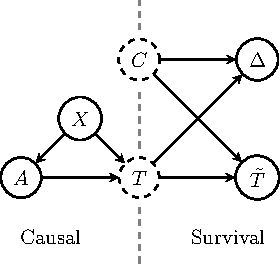
\includegraphics[width=0.4\textwidth,height=\textheight]{causal_survival_obs_indep.pdf}

}

\caption{\label{fig-causalgraph_obs_ind}Causal graph in observational
survival data with independent censoring.}

\end{figure}%

Under Assumption \ref{eq-independantcensoring}, we saw in
Section~\ref{sec-theoryRCT_indc} that the Kaplan-Meier estimator could
conveniently handle censoring. Building on Equation~\ref{eq-kmcond}, we
can write \[
S^{(1)}(t) = \mathbb{E}\left[\frac{\mathbb{E}[\mathbb{I}\{A=1,T > t\}|X]}{\mathbb{E}[\mathbb{I}\{A=1\}|X]} \right]=\mathbb{E}\left[\frac{A\mathbb{I}\{T > t\}}{e(X)} \right],
\] which suggests to adapt the classical KM estimator by reweighting it
by the propensity score. The use of propensity score in causal inference
has been initially introduced by Rosenbaum and Rubin (1983) and further
developed in Hirano, Imbens, and Ridder (2003). It was extended to
survival analysis by Xie and Liu (2005) through the adjusted
Kaplan-Meier estimator as defined below.

\begin{definition}[]\protect\hypertarget{def-iptwkm}{}\label{def-iptwkm}

(IPTW Kaplan-Meier estimator) We let \(\widehat e(\cdot)\) be an
estimator of the propensity score \(e(\cdot)\). We introduce

\begin{align*}
D_k^{\mathrm{IPTW}}(a) &:= \sum_{i=1}^n \left(\frac{a}{\widehat e(X_i)}+\frac{1-a}{1- \widehat e(X_i)}\right)\mathbb{I}(\widetilde T_i = t_k, \Delta_i = 1, A_i=a) \\
\quad\text{and}\quad N^{\mathrm{IPTW}}_k(a) &:= \sum_{i=1}^n \left(\frac{a}{\widehat e(X_i)}+\frac{1-a}{1- \widehat e(X_i)}\right) \mathbb{I}(\widetilde T_i \geqslant t_k, A_i=a),
\end{align*}

be the numbers of deaths and of individual at risk at time \(t_k\),
reweighted by the propensity score. The Inverse-Probability-of-Treatment
Weighting (IPTW) version of the KM estimator is then defined as:
\begin{equation}\phantomsection\label{eq-IPTWKM}{
\begin{aligned}
\widehat{S}_{\mathrm{IPTW}}(t | A=a) &= \prod_{t_k \leqslant t}\left(1-\frac{D_k^{\mathrm{IPTW}}(a)}{N_k^{\mathrm{IPTW}}(a)}\right). 
\end{aligned}
}\end{equation}

\end{definition}

We let \(S^*_{\mathrm{IPTW}}(t | A=a)\) be the oracle KM-estimator
defined as above with \(\widehat e(\cdot) = e(\cdot)\). Although the
reweighting slightly changes the analysis, the good properties of the
classical KM carry on to this setting.

\begin{proposition}[]\protect\hypertarget{prp-iptwkm}{}\label{prp-iptwkm}

Under Assumptions
\ref{eq-sutva}, \ref{eq-unconf}, \ref{eq-positivitytreat}, \ref{eq-independantcensoring}
and \ref{eq-poscen} The oracle IPTW Kaplan-Meier estimator
\(S^*_{\mathrm{IPTW}}(t | A=a)\) is a strongly consistent and
asymptotically normal estimator of \(S^{(a)}(t)\).

\end{proposition}

The proof of this result simply relies again on the law of large number
and the \(\delta\)-method and can be found in Section~\ref{sec-proof31}.
Because now \(S^*_{\mathrm{IPTW}}\) is a continuous function of
\(e(\cdot)\), and because \(e\) and \(1-e\) are lower-bounded as per
Assumptions \ref{eq-positivitytreat}, we easily derive the following
corollary.

\begin{corollary}[]\protect\hypertarget{cor-iptwkm}{}\label{cor-iptwkm}

Under the same assumptions as Proposition~\ref{prp-iptwkm}, if
\(\widehat e(\cdot)\) satisfies \(\|\widehat e-e\|_{\infty} \to 0\)
almost surely (resp. in probability), then the IPTW Kaplan-Meier
estimator \(\hat S_{\mathrm{IPTW}}(t | A=a)\) is a strongly (resp.
weakly) consistent estimator of \(S^{(a)}(t)\).

\end{corollary}

The resulting RMST estimator simply takes the form:
\begin{equation}\phantomsection\label{eq-RMST_IPTWKM}{
\widehat{\theta}_{\mathrm{IPTW-KM}} = \int_{0}^{\tau}\widehat{S}_{\mathrm{IPTW}}(t|A=1)-\widehat{S}_{\mathrm{IPTW}}(t|A=0)dt.
}\end{equation} which will be consistent under the same Assumptions as
the previous Corollary. Note that, we are not aware of any formal
results concerning the bias and the asymptotic variance of the oracle
estimator \(S^*_{\mathrm{IPTW}}(t | A=a)\), and we refer to Xie and Liu
(2005) for heuristics concerning these questions.

\subsection{Conditional independent censoring}\label{sec-obscondcens}

Under Assumptions \ref{eq-unconf} (uncounfoundedness) and
\ref{eq-condindepcensoring} (conditional independent censoring), the
causal effect is affected both by confounding variables and by
conditional censoring. The associated causal graph is depicted in
Figure~\ref{fig-causalgraph_obs_dep}. In this setting, one can still use
the \(G\)-formula exactly as in Section~\ref{sec-Gformula}.

A natural alternative approach is to weight the IPCW and BJ
transformations from Section~\ref{sec-unbiasedtransfo} by the propensity
score to disentangle both confounding effects and censoring at the same
time.

\begin{figure}

\centering{

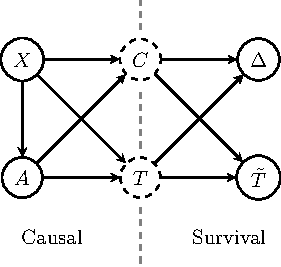
\includegraphics[width=0.4\textwidth,height=\textheight]{causal_survival_obs_dep.pdf}

}

\caption{\label{fig-causalgraph_obs_dep}Causal graph in observational
survival data with dependent censoring.}

\end{figure}%

We mention that the G-formula approach developed in
Section~\ref{sec-Gformula} does work in that context. In particular,
Chen and Tsiatis (2001) prove consistency and asymptotic normality
results for Cox estimators in a observational study, and they give an
explicit formulation of the asymptotic variance as a function of the
parameters of the Cox model. In the non-parametric world, Foster,
Taylor, and Ruberg (2011) and Künzel et al. (2019) empirically study
this estimator using survival forests, with the former employing it as a
T-learner (referred to as \emph{Virtual Twins}) and the latter as an
S-learner.

\subsubsection{IPTW-IPCW
transformations}\label{iptw-ipcw-transformations}

One can check that the IPCW transformation as introduced in
Equation~\ref{eq-defipcw} is also a censoring unbiased transformation in
that context.

\begin{proposition}[]\protect\hypertarget{prp-iptwipcw}{}\label{prp-iptwipcw}

Under Assumptions
\ref{eq-sutva}, \ref{eq-unconf}, \ref{eq-positivitytreat}, \ref{eq-condindepcensoring}
and \ref{eq-positivitycensoring}, the IPTW-IPCW transform
\ref{eq-defipcw} is a censoring unbiased transformation in the sense of
Equation~\ref{eq-cut}.

\end{proposition}

The proof of Proposition~\ref{prp-iptwipcw} can be found in
Section~\ref{sec-proof32}. Deriving an estimator of the difference in
RMST is however slightly different in that context. In particular,
Equation~\ref{eq-cutcond} rewrites \[
\mathbb{E}[\mathbb{E}[T^*|X,A=1]] = \mathbb{E}\left[\frac{A}{e(X)} T^*\right],
\] Which in turn suggests to define
\begin{equation}\phantomsection\label{eq-iptwipcw}{
\widehat\theta_{\mathrm{IPTW-IPCW}} = \frac1n\sum_{i=1}^n  \left(\frac{A}{e(X)}-\frac{1-A}{1-e(X)} \right) T^*_{\mathrm{IPCW},i}.
}\end{equation}

This transformation now depends on two nuisance parameters, namely the
conditional survival function of the censoring (through
\(T^*_{\mathrm{IPCW}}\)) and the propensity score. Once estimators of
these quantities are provided, one could look at the corresponding
quantity computed with these estimators.

\begin{proposition}[]\protect\hypertarget{prp-consiptwipcw}{}\label{prp-consiptwipcw}

Under Assumptions
\ref{eq-sutva}, \ref{eq-unconf}, \ref{eq-positivitytreat}, \ref{eq-condindepcensoring}
and \ref{eq-positivitycensoring}, and if \(\widehat G(\cdot|X,A)\) and
\(\widehat e (\cdot)\) are uniformly weakly (resp. strongly) consistent
estimators, then estimator \ref{eq-iptwipcw} defined with \(\widehat e\)
and \(\widehat G\) is a weakly (resp. strongly) consistent estimator of
the difference in RMST.

\end{proposition}

The proof of Proposition~\ref{prp-consiptwipcw} can be found in
Section~\ref{sec-proof32}. We can also use the same strategy as for the
IPCW transformation and incorporate the new weights into a Kaplan-Meier
estimator.

\begin{definition}[]\protect\hypertarget{def-iptwipcwkm}{}\label{def-iptwipcwkm}

(IPTW-IPCW-Kaplan-Meier) We let again \(\widehat G(\cdot|X,A)\) and
\(\widehat e(\cdot)\) be estimators of the conditional censoring
survival function and of the propensity score. We introduce

\begin{align*}
D_k^{\mathrm{IPTW-IPCW}}(a) &:= \sum_{i=1}^n \left(\frac{A_i}{\widehat e(X_i)}+\frac{1-A_i}{1-\widehat e(X_i)} \right)\frac{\Delta_i^\tau}{\widehat G(\widetilde T_i \wedge\tau | X_i,A=a)} \mathbb{I}(\widetilde T_i = t_k, A_i=a) \\
\quad\text{and}\quad N^{\mathrm{IPTW-IPCW}}_k(a) &:= \sum_{i=1}^n \left(\frac{A_i}{\widehat e(X_i)}+\frac{1-A_i}{1-\widehat e(X_i)} \right)\frac{\Delta_i^\tau}{\widehat G(\widetilde T_i \wedge\tau | X_i,A=a)} \mathbb{I}(\widetilde T_i \geqslant t_k, A_i=a),
\end{align*}

be the weight-corrected numbers of deaths and of individual at risk at
time \(t_k\). The IPTW-IPCW version of the KM estimator is then defined
as: \[
\begin{aligned}
\widehat{S}_{\mathrm{IPTW-IPCW}}(t | A=a) &= \prod_{t_k \leqslant t}\left(1-\frac{D_k^{\mathrm{IPTW-IPCW}}(a)}{N_k^{\mathrm{IPTW-IPCW}}(a)}\right). 
\end{aligned}
\]

\end{definition}

The difference in RMST estimated with IPTW-IPCW-Kaplan-Meier survival
curves is then simply as

\begin{equation}\phantomsection\label{eq-RMST_IPTW_IPCWKM}{
\widehat{\theta}_{\mathrm{IPTW-IPCW-KM}} = \int_{0}^{\tau}\widehat{S}_{\mathrm{IPTW-IPCW}}(t|A=1)-\widehat{S}_{\mathrm{IPTW-IPCW}}(t|A=0)dt.
}\end{equation}

\begin{proposition}[]\protect\hypertarget{prp-iptwipcwkm}{}\label{prp-iptwipcwkm}

Under Assumptions
\ref{eq-sutva}, \ref{eq-unconf}, \ref{eq-positivitytreat}, \ref{eq-condindepcensoring}
and \ref{eq-positivitycensoring}, and for all \(t \in [0,\tau]\), if the
oracle estimator \(S^*_{\mathrm{IPTW-IPCW}}(t | A=a)\) defined as in
Definition~\ref{def-iptwipcwkm} with
\(\widehat G(\cdot|A,X) = G(\cdot|A,X)\) and \(\widehat e = e\) is a
strongly consistent and asymptotically normal estimator of
\(S^{(a)}(t)\) .

\end{proposition}

The proof of Proposition~\ref{prp-iptwipcwkm} can be found in
Section~\ref{sec-proof32}. Under consistency of the estimators of the
nuisance parameters, the previous proposition implies that this
reweighted Kaplan-Meier is a consistent estimator of the survival curve,
which in turn implies consistency of
\(\widehat{\theta}_{\mathrm{IPTW-IPCW-KM}}\).

\begin{corollary}[]\protect\hypertarget{cor-consiptwipcwkm}{}\label{cor-consiptwipcwkm}

Under Assumptions
\ref{eq-sutva}, \ref{eq-unconf}, \ref{eq-positivitytreat}, \ref{eq-condindepcensoring}
and \ref{eq-positivitycensoring}, and for all \(t \in [0,\tau]\), if the
nuisance estimators \(\widehat G(\cdot|A,X)\) and \(\widehat e\) are
weakly (resp. strongly) uniformly consistent, then
\(\widehat{S}_{\mathrm{IPTW-IPCW}}(t | A=a)\) is a weakly (resp.
strongly) consistent estimator of \(S^{(a)}(t)\).

\end{corollary}

We are not aware of general formula for the asymptotic variances in this
context. We mention nonetheless that Schaubel and Wei (2011) have been
able to derive asymptotic laws in this framework in the particular case
of Cox-models.

\subsubsection{IPTW-BJ transformations}\label{iptw-bj-transformations}

Like IPCW tranformation, BJ transformation is again a censoring unbiased
transformation in an observational context.

\begin{proposition}[]\protect\hypertarget{prp-iptwbj}{}\label{prp-iptwbj}

Under Assumptions
\ref{eq-sutva}, \ref{eq-unconf}, \ref{eq-positivitytreat}, \ref{eq-condindepcensoring}
and \ref{eq-positivitycensoring}, the IPTW-BJ transform \ref{eq-defbj}
is a censoring unbiased transformation in the sense of
Equation~\ref{eq-cut}.

\end{proposition}

The proof of Proposition~\ref{prp-iptwbj} can be found in
Section~\ref{sec-proof32}. The corresponding estimator of the difference
in RMST is \begin{equation}\phantomsection\label{eq-iptwbj}{
\hat \theta_{\mathrm{IPTW-BJ}} = \frac1n\sum_{i=1}^n  \left(\frac{A}{e(X)}-\frac{1-A}{1-e(X)} \right) T^*_{\mathrm{BJ},i}.
}\end{equation}

This transformation depends on the conditional survival function \(S\)
(through \(T^*_{\mathrm{BJ}}\)) and the propensity score. Consistency of
the nuisance parameter estimators implies again consistency of the RMST
estimator.

\begin{proposition}[]\protect\hypertarget{prp-consiptwbj}{}\label{prp-consiptwbj}

Under Assumptions
\ref{eq-sutva}, \ref{eq-unconf}, \ref{eq-positivitytreat}, \ref{eq-condindepcensoring}
and \ref{eq-positivitycensoring}, and if \(\widehat S(\cdot|X,A)\) and
\(\widehat e (\cdot)\) are uniformly weakly (resp. strongly) consistent
estimators, then \(\widehat\theta_{\mathrm{IPTW-BJ}}\) defined with
\(\widehat S\) and \(\widehat e\) is a weakly (resp. strongly)
consistent estimator of the RMST.

\end{proposition}

The proof of Proposition~\ref{prp-consiptwbj} can be found in
Section~\ref{sec-proof32}.

\subsubsection{Double augmented corrections}\label{sec-AIPTW_AIPCW}

Building on the classical doubly-robust AIPTW estimator from causal
inference (Robins, Rotnitzky, and Zhao 1994), we could incorporate the
doubly-robust transformations of Section~\ref{sec-tdr} to obtain a
\emph{quadruply robust} tranformation \[
\Delta^*_{\mathrm{QR}} = \Delta^*_{\mathrm{QR}}(G,S,\mu,e)  := \left(\frac{A}{e(X)}-\frac{1-A}{1-e(X)}\right)(T^*_{\mathrm{DR}}(G,S)-\mu(X,A))+\mu(X,1)-\mu(X,0),
\] where we recall that \(T^*_{\mathrm{DR}}\) is defined in
Section~\ref{sec-tdr}. This transformations depends on four nuisance
parameters: \(G\) and \(S\) through \(T^*_{\mathrm{DR}}\), and now the
propensity score \(e\) and the conditional response \(\mu\). This
transformation doesn't really fall into the scope of censoring unbiased
transform, but it is easy to show that \(\Delta^*_{\mathrm{QR}}\) is
quadruply robust in the following sense.

\begin{proposition}[]\protect\hypertarget{prp-tqr}{}\label{prp-tqr}

Let \(F,R\) be two conditional survival function, \(p\) be a propensity
score, and \(\nu\) be a conditional response. Then, under the same
assumption on \(F,R\) as in Proposition~\ref{prp-tdr}, and under
Assumptions
\ref{eq-sutva}, \ref{eq-unconf}, \ref{eq-positivitytreat}, \ref{eq-condindepcensoring}
and \ref{eq-positivitycensoring}, the transformations
\(\Delta^*_{\mathrm{QR}} = \Delta^*_{\mathrm{QR}}(F,R,p,\nu)\)
satisfies, fo \(a \in {0,1}\), \[
\mathbb{E}[ \Delta^*_\mathrm{QR} |X] = \mathbb{E}[T(1)\wedge \tau-T(0)\wedge \tau |X]\quad\text{if}\quad  
\begin{cases} F = G \quad &\text{or}\quad R=S \quad \text{and} \\
p=e \quad &\text{or}\quad \nu=\mu.
\end{cases}
\]

\end{proposition}

This result is similar to Ozenne et al. (2020), Thm 1, and its proof can
be found in Section~\ref{sec-proof32}. Based on estimators
\((\widehat G, \widehat S, \widehat\mu, \widehat e)\) of
\((G,S,\mu,e)\), one can then propose the following estimator of the
RMST, coined the AIPTW-AIPCW estimator in Ozenne et al. (2020):
\begin{equation}\phantomsection\label{eq-AIPTW_AIPCW}{
\begin{aligned}
\widehat\theta_{\mathrm{AIPTW-AIPCW}} &:= \frac1n \sum_{i=1}^n \Delta_{\mathrm{QR},i}^*(\widehat G, \widehat S, \widehat\mu, \widehat e)
\\
&=\frac1n \sum_{i=1}^n \left(\frac{A_i}{\widehat e(X_i)}-\frac{1-A_i}{1-\widehat e(X_i)}\right)(T^*_{\mathrm{DR}}(\widehat G,\widehat S)_i-\widehat\mu(X_i,A_i)) + \widehat\mu(X_i,1)-\widehat\mu(X_i,0).
\end{aligned}
}\end{equation} This estimator enjoys good asymptotic properties under
parametric models, as detailed in Ozenne et al. (2020).

\section{Implementation}\label{implementation}

In this section, we first summarize the various estimators and their
properties. We then provide custom implementations for all estimators,
even those already available in existing packages. These manual
implementations serve two purposes: first, to make the methods
accessible to the community when no existing implementation is
available; and second, to facilitate a deeper understanding of the
methods by detailing each step, even when a package solution exists.
Finally, we present the packages available for directly computing
\(\theta_{\mathrm{RMST}}\).

\subsection{Summary of the estimators}\label{sec-summary}

Table~\ref{tbl-nuisance} provides an overview of the estimators
introduced in this paper, along with the corresponding nuisance
parameters needed for their estimation and an overview of their
statistical properties in particular regarding their sensitivity to
misspecification of the nuisance parameters.

\begin{longtable}[]{@{}
  >{\raggedright\arraybackslash}p{(\columnwidth - 16\tabcolsep) * \real{0.2500}}
  >{\raggedright\arraybackslash}p{(\columnwidth - 16\tabcolsep) * \real{0.0625}}
  >{\raggedright\arraybackslash}p{(\columnwidth - 16\tabcolsep) * \real{0.0625}}
  >{\raggedright\arraybackslash}p{(\columnwidth - 16\tabcolsep) * \real{0.0625}}
  >{\raggedright\arraybackslash}p{(\columnwidth - 16\tabcolsep) * \real{0.0625}}
  >{\raggedright\arraybackslash}p{(\columnwidth - 16\tabcolsep) * \real{0.1250}}
  >{\raggedright\arraybackslash}p{(\columnwidth - 16\tabcolsep) * \real{0.1250}}
  >{\raggedright\arraybackslash}p{(\columnwidth - 16\tabcolsep) * \real{0.1250}}
  >{\raggedright\arraybackslash}p{(\columnwidth - 16\tabcolsep) * \real{0.1250}}@{}}
\caption{Estimators of the difference in RMST and nuisance parameters
needed to compute each estimator. Empty boxes indicate that the nuisance
parameter is not needed in the estimator thus misspecification has no
impact. Estimators in italic are those that are already implemented in
available packages.}\label{tbl-nuisance}\tabularnewline
\toprule\noalign{}
\begin{minipage}[b]{\linewidth}\raggedright
Estimator
\end{minipage} & \begin{minipage}[b]{\linewidth}\raggedright
RCT
\end{minipage} & \begin{minipage}[b]{\linewidth}\raggedright
Obs
\end{minipage} & \begin{minipage}[b]{\linewidth}\raggedright
Ind Cens
\end{minipage} & \begin{minipage}[b]{\linewidth}\raggedright
Dep Cens
\end{minipage} & \begin{minipage}[b]{\linewidth}\raggedright
Outcome model
\end{minipage} & \begin{minipage}[b]{\linewidth}\raggedright
Censoring model
\end{minipage} & \begin{minipage}[b]{\linewidth}\raggedright
Treatment model
\end{minipage} & \begin{minipage}[b]{\linewidth}\raggedright
Robustness
\end{minipage} \\
\midrule\noalign{}
\endfirsthead
\toprule\noalign{}
\begin{minipage}[b]{\linewidth}\raggedright
Estimator
\end{minipage} & \begin{minipage}[b]{\linewidth}\raggedright
RCT
\end{minipage} & \begin{minipage}[b]{\linewidth}\raggedright
Obs
\end{minipage} & \begin{minipage}[b]{\linewidth}\raggedright
Ind Cens
\end{minipage} & \begin{minipage}[b]{\linewidth}\raggedright
Dep Cens
\end{minipage} & \begin{minipage}[b]{\linewidth}\raggedright
Outcome model
\end{minipage} & \begin{minipage}[b]{\linewidth}\raggedright
Censoring model
\end{minipage} & \begin{minipage}[b]{\linewidth}\raggedright
Treatment model
\end{minipage} & \begin{minipage}[b]{\linewidth}\raggedright
Robustness
\end{minipage} \\
\midrule\noalign{}
\endhead
\bottomrule\noalign{}
\endlastfoot
\emph{Unadjusted KM} & \(\color{green}X\) & & \(\color{green}X\) & & & &
& \\
IPCW-KM & \(\color{green}X\) & & \(\color{green}X\) & \(\color{green}X\)
& & \(G\) & & \\
BJ & \(\color{green}X\) & & \(\color{green}X\) & \(\color{green}X\) &
\(S\) & & & \\
\emph{IPTW-KM} & \(\color{green}X\) & \(\color{green}X\) &
\(\color{green}X\) & & & & \(e\) & \\
IPCW-IPTW-KM & \(\color{green}X\) & \(\color{green}X\) &
\(\color{green}X\) & \(\color{green}X\) & & \(G\) & \(e\) & \\
IPTW-BJ & \(\color{green}X\) & \(\color{green}X\) & \(\color{green}X\) &
\(\color{green}X\) & \(S\) & & \(e\) & \\
\emph{G-formula} & \(\color{green}X\) & \(\color{green}X\) &
\(\color{green}X\) & \(\color{green}X\) & \(\mu\) & & & \\
AIPTW-AIPCW & \(\color{green}X\) & \(\color{green}X\) &
\(\color{green}X\) & \({\color{green}X}\) & \(S,\mu\) & \(G\) & \(e\) &
\(\color{green}X\) (Prp \ref{prp-tqr}) \\
\end{longtable}

\subsection{Implementation of the
estimators}\label{implementation-of-the-estimators}

Across different implementations, we use the following shared functions
provided in the \(\texttt{utilitary.R}\) file.

\begin{itemize}
\item
  \(\texttt{estimate\_propensity\_score}\): function to estimate
  propensity scores \(e(X)\) using either parametric (i.e.~logistic
  regression with the argument \(\texttt{type\_of\_model = "glm"}\)) or
  non-parametric methods (i.e.~probability forest with the argument
  \(\texttt{type\_of\_model ="probability forest"}\) based on the
  \(\texttt{probability\_forest}\) function from the
  \href{https:\%20//cran.r-project.org/web/packages/grf/index.html}{grf}
  (Tibshirani et al. 2017) package). This latter can include
  cross-fitting (\(\texttt{n.folds\>1}\)).
\item
  \(\texttt{estimate\_survival\_function}\): function to estimate the
  conditional survival model, which supports either Cox models (argument
  \(\texttt{type\_of\_model = "cox"}\)) or survival forests (argument
  \(\texttt{type\_of\_model = "survival forest"}\)) which uses the
  function \(\texttt{survival\_forest}\) from the
  \href{https:\%20//cran.r-project.org/web/packages/grf/index.html}{grf}
  (Tibshirani et al. 2017) package. This latter can include
  cross-fitting (\(\texttt{n.folds\>1}\)). The estimation can be done
  with a single learner (argument \(\texttt{learner = "S-learner"}\)) or
  two learners (argument \(\texttt{learner = "T-learner"}\)).
\item
  \(\texttt{estimate\_hazard\_function}\): function to estimate the
  instantaneous hazard function by deriving the cumulative hazard
  function at each time point. This cumulative hazard function is
  estimated from the negative logarithm of the survival function.
\item
  \(\texttt{Q\_t\_hat}\): function to estimate the remaining survival
  function at all time points and for all individuals which uses the
  former \(\texttt{estimate\_survival\_function}\).
\item
  \(\texttt{Q\_Y}\): function to select the value of the remaining
  survival function from \(\texttt{Q\_t\_hat}\) at the specific
  time-to-event.
\item
  \(\texttt{integral\_rectangles}\): function to estimate the integral
  of a decreasing step function using the rectangle method.
\item
  \(\texttt{expected\_survival}\): function to estimate the integral
  with \(x,y\) coordinate (estimated survival function) using the
  trapezoidal method.
\item
  \(\texttt{integrate}\): function to estimate the integral at specific
  time points \(\texttt{Y.grid}\) of a given \(\texttt{integrand}\)
  function which takes initially its values on \(\texttt{times}\) using
  the trapezoidal method.
\end{itemize}

\textbf{Unadjusted Kaplan-Meier}

Although Kaplan-Meier is implemented in the \(\texttt{survival}\)
package (Therneau 2001), we provide a custom implementation,
\(\texttt{Kaplan\_meier\_handmade}\), for completeness. The difference
in Restricted Mean Survival Time, estimated using Kaplan-Meier as in
Equation~\ref{eq-thetaunadjKM} can then be calculated with the
\(\texttt{RMST\_1}\) function.

\begin{Shaded}
\begin{Highlighting}[]
\FunctionTok{source}\NormalTok{(}\StringTok{"utilitary.R"}\NormalTok{)}
\CommentTok{\# Kaplan{-}Meier estimator handmade implementation}
\CommentTok{\# The database \textquotesingle{}data\textquotesingle{} must be in the same form as that shown in }
\CommentTok{\# notation (Table 1) and with the same variable names (status, T\_obs) }
\NormalTok{Kaplan\_meier\_handmade }\OtherTok{\textless{}{-}} \ControlFlowTok{function}\NormalTok{(data, }
                                  \AttributeTok{status =}\NormalTok{ data}\SpecialCharTok{$}\NormalTok{status, }
                                  \AttributeTok{T\_obs =}\NormalTok{ data}\SpecialCharTok{$}\NormalTok{T\_obs) \{}
  \CommentTok{\# Sort unique observed times}
\NormalTok{  Y.grid }\OtherTok{\textless{}{-}} \FunctionTok{sort}\NormalTok{(}\FunctionTok{unique}\NormalTok{(T\_obs))}
  
  \CommentTok{\# Initialize vectors for number of events, number at risk, and survival }
  \CommentTok{\# probability}
\NormalTok{  d }\OtherTok{\textless{}{-}} \FunctionTok{rep}\NormalTok{(}\ConstantTok{NA}\NormalTok{, }\FunctionTok{length}\NormalTok{(Y.grid))  }\CommentTok{\# Number of events at time Y.grid[i]}
\NormalTok{  n }\OtherTok{\textless{}{-}} \FunctionTok{rep}\NormalTok{(}\ConstantTok{NA}\NormalTok{, }\FunctionTok{length}\NormalTok{(Y.grid))  }\CommentTok{\# Number at risk just before time Y.grid[i]}
\NormalTok{  S }\OtherTok{\textless{}{-}} \FunctionTok{rep}\NormalTok{(}\ConstantTok{NA}\NormalTok{, }\FunctionTok{length}\NormalTok{(Y.grid))  }\CommentTok{\# Survival probability at time Y.grid[i]}
  
  \CommentTok{\# Loop over each unique observed time}
  \ControlFlowTok{for}\NormalTok{ (i }\ControlFlowTok{in} \DecValTok{1}\SpecialCharTok{:}\FunctionTok{length}\NormalTok{(Y.grid)) \{}
\NormalTok{    d[i] }\OtherTok{\textless{}{-}} \FunctionTok{sum}\NormalTok{(T\_obs }\SpecialCharTok{==}\NormalTok{ Y.grid[i] }\SpecialCharTok{\&}\NormalTok{ status }\SpecialCharTok{==} \DecValTok{1}\NormalTok{, }\AttributeTok{na.rm =} \ConstantTok{TRUE}\NormalTok{)  }\CommentTok{\# Count events}
\NormalTok{    n[i] }\OtherTok{\textless{}{-}} \FunctionTok{sum}\NormalTok{(T\_obs }\SpecialCharTok{\textgreater{}=}\NormalTok{ Y.grid[i])  }\CommentTok{\# Count at risk}
    
    \CommentTok{\# Calculate survival probability}
\NormalTok{    S[i] }\OtherTok{\textless{}{-}} \FunctionTok{cumprod}\NormalTok{(}\DecValTok{1} \SpecialCharTok{{-}}\NormalTok{ d }\SpecialCharTok{/}\NormalTok{ n)[i]}
\NormalTok{  \}}
  
  \CommentTok{\# Create a dataframe with the results}
\NormalTok{  df }\OtherTok{\textless{}{-}} \FunctionTok{data.frame}\NormalTok{(}\AttributeTok{d =}\NormalTok{ d, }\AttributeTok{n =}\NormalTok{ n, }\AttributeTok{S =}\NormalTok{ S, }\AttributeTok{T =}\NormalTok{ Y.grid)}
  
  \FunctionTok{return}\NormalTok{(df)}
\NormalTok{\}}


\CommentTok{\# Function to calculate RMST (Restricted Mean Survival Time):}
\CommentTok{\# Two possibilities for computing RMST: }
\CommentTok{\# {-} in using directly S\_A1 and S\_A0 (survival function of treated and control)}
\CommentTok{\# {-} in using the dataframe and the function computes the survival functions}
\NormalTok{RMST\_1 }\OtherTok{\textless{}{-}} \ControlFlowTok{function}\NormalTok{(}\AttributeTok{data =} \ConstantTok{NULL}\NormalTok{, }\AttributeTok{A1 =} \DecValTok{1}\NormalTok{, }\AttributeTok{A0 =} \DecValTok{0}\NormalTok{, tau, }\AttributeTok{S\_A1 =} \ConstantTok{NULL}\NormalTok{, }\AttributeTok{S\_A0 =} \ConstantTok{NULL}\NormalTok{) \{}
  \ControlFlowTok{if}\NormalTok{ (}\FunctionTok{is.null}\NormalTok{(S\_A1) }\SpecialCharTok{\&} \FunctionTok{is.null}\NormalTok{(S\_A0)) \{}
    \CommentTok{\# Subset data for treatment groups}
\NormalTok{    data1 }\OtherTok{\textless{}{-}}\NormalTok{ data[data}\SpecialCharTok{$}\NormalTok{A }\SpecialCharTok{==}\NormalTok{ A1,]}
\NormalTok{    data0 }\OtherTok{\textless{}{-}}\NormalTok{ data[data}\SpecialCharTok{$}\NormalTok{A }\SpecialCharTok{==}\NormalTok{ A0,]}
    
    \CommentTok{\# Calculate Kaplan{-}Meier survival estimates}
\NormalTok{    S\_A1 }\OtherTok{\textless{}{-}} \FunctionTok{Kaplan\_meier\_handmade}\NormalTok{(data1, }\AttributeTok{status =}\NormalTok{ data1}\SpecialCharTok{$}\NormalTok{status, }
                                  \AttributeTok{T\_obs =}\NormalTok{ data1}\SpecialCharTok{$}\NormalTok{T\_obs)}
\NormalTok{    S\_A0 }\OtherTok{\textless{}{-}} \FunctionTok{Kaplan\_meier\_handmade}\NormalTok{(data0, }\AttributeTok{status =}\NormalTok{ data0}\SpecialCharTok{$}\NormalTok{status, }
                                  \AttributeTok{T\_obs =}\NormalTok{ data0}\SpecialCharTok{$}\NormalTok{T\_obs)}
    
    \CommentTok{\# Restrict observations to those less than or equal to tau}
\NormalTok{    Y.grid1 }\OtherTok{\textless{}{-}}\NormalTok{ data1}\SpecialCharTok{$}\NormalTok{T\_obs[data1}\SpecialCharTok{$}\NormalTok{T\_obs }\SpecialCharTok{\textless{}=}\NormalTok{ tau]}
\NormalTok{    Y.grid0 }\OtherTok{\textless{}{-}}\NormalTok{ data0}\SpecialCharTok{$}\NormalTok{T\_obs[data0}\SpecialCharTok{$}\NormalTok{T\_obs }\SpecialCharTok{\textless{}=}\NormalTok{ tau]}
\NormalTok{  \} }\ControlFlowTok{else}\NormalTok{ \{}
    \CommentTok{\# Restrict observations to those less than or equal to tau}
\NormalTok{    Y.grid1 }\OtherTok{\textless{}{-}}\NormalTok{ S\_A1}\SpecialCharTok{$}\NormalTok{T[S\_A1}\SpecialCharTok{$}\NormalTok{T }\SpecialCharTok{\textless{}=}\NormalTok{ tau]}
\NormalTok{    Y.grid0 }\OtherTok{\textless{}{-}}\NormalTok{ S\_A0}\SpecialCharTok{$}\NormalTok{T[S\_A0}\SpecialCharTok{$}\NormalTok{T }\SpecialCharTok{\textless{}=}\NormalTok{ tau]}
\NormalTok{  \}}
  
  \CommentTok{\# Filter survival estimates to restricted observations}
\NormalTok{  S\_A1 }\OtherTok{\textless{}{-}}\NormalTok{ S\_A1 }\SpecialCharTok{\%\textgreater{}\%}
\NormalTok{    dplyr}\SpecialCharTok{::}\FunctionTok{filter}\NormalTok{(T }\SpecialCharTok{\%in\%}\NormalTok{ Y.grid1)}
\NormalTok{  S\_A0 }\OtherTok{\textless{}{-}}\NormalTok{ S\_A0 }\SpecialCharTok{\%\textgreater{}\%}
\NormalTok{    dplyr}\SpecialCharTok{::}\FunctionTok{filter}\NormalTok{(T }\SpecialCharTok{\%in\%}\NormalTok{ Y.grid0)}
  
  \CommentTok{\# Check if there is any event at tau for S\_A1}
  \ControlFlowTok{if}\NormalTok{ (}\SpecialCharTok{!}\FunctionTok{any}\NormalTok{(S\_A1}\SpecialCharTok{$}\NormalTok{T }\SpecialCharTok{==}\NormalTok{ tau)) \{}
\NormalTok{    new\_row }\OtherTok{\textless{}{-}} \FunctionTok{tibble}\NormalTok{(}\AttributeTok{T =}\NormalTok{ tau, }\AttributeTok{S =}\NormalTok{ S\_A1}\SpecialCharTok{$}\NormalTok{S[}\FunctionTok{nrow}\NormalTok{(S\_A1)])}
\NormalTok{    S\_A1 }\OtherTok{\textless{}{-}}\NormalTok{ dplyr}\SpecialCharTok{::}\FunctionTok{bind\_rows}\NormalTok{(S\_A1, new\_row)}
\NormalTok{  \}}
  
  \CommentTok{\# Check if there is any event at tau for S\_A0}
  \ControlFlowTok{if}\NormalTok{ (}\SpecialCharTok{!}\FunctionTok{any}\NormalTok{(S\_A0}\SpecialCharTok{$}\NormalTok{T }\SpecialCharTok{==}\NormalTok{ tau)) \{}
\NormalTok{    new\_row }\OtherTok{\textless{}{-}} \FunctionTok{tibble}\NormalTok{(}\AttributeTok{T =}\NormalTok{ tau, }\AttributeTok{S =}\NormalTok{ S\_A0}\SpecialCharTok{$}\NormalTok{S[}\FunctionTok{nrow}\NormalTok{(S\_A0)])}
\NormalTok{    S\_A0 }\OtherTok{\textless{}{-}}\NormalTok{ dplyr}\SpecialCharTok{::}\FunctionTok{bind\_rows}\NormalTok{(S\_A0, new\_row)}
\NormalTok{  \}}

  \CommentTok{\# Calculate integrals from 0 to tau of survival probabilities}
\NormalTok{  intA1 }\OtherTok{\textless{}{-}} \FunctionTok{integral\_rectangles}\NormalTok{(S\_A1}\SpecialCharTok{$}\NormalTok{T, S\_A1}\SpecialCharTok{$}\NormalTok{S)}
\NormalTok{  intA0 }\OtherTok{\textless{}{-}} \FunctionTok{integral\_rectangles}\NormalTok{(S\_A0}\SpecialCharTok{$}\NormalTok{T, S\_A0}\SpecialCharTok{$}\NormalTok{S)}
\NormalTok{  RMST1 }\OtherTok{\textless{}{-}}\NormalTok{ intA1 }\SpecialCharTok{{-}}\NormalTok{ intA0}
  
  \FunctionTok{return}\NormalTok{(}\FunctionTok{list}\NormalTok{(}\AttributeTok{RMST=}\NormalTok{RMST1, }\AttributeTok{intA1=}\NormalTok{intA1,}\AttributeTok{intA0=}\NormalTok{intA0))}
\NormalTok{\}}
\end{Highlighting}
\end{Shaded}

As an alternative, one can also use the \(\texttt{survfit}\) function in
the survival package (Therneau 2001) for Kaplan-Meier and specify the
\(\texttt{rmean}\) argument equal to \(\tau\) in the corresponding
summary function:

\begin{Shaded}
\begin{Highlighting}[]
\CommentTok{\# Alternative code to estimate Kaplan{-}Meier estimator with survival package}
\CommentTok{\# instead of handmade KM}
\NormalTok{RMST\_alternative }\OtherTok{\textless{}{-}} \ControlFlowTok{function}\NormalTok{(data, }\AttributeTok{A1 =} \DecValTok{1}\NormalTok{, }\AttributeTok{A0 =} \DecValTok{0}\NormalTok{, tau)\{}
  \CommentTok{\# Estimate Kaplan{-}Meier estimator with survfit function on data subset}
   \CommentTok{\# Groupe A = 0}
\NormalTok{  fit0 }\OtherTok{\textless{}{-}} \FunctionTok{survfit}\NormalTok{(}\FunctionTok{Surv}\NormalTok{(T\_obs, status) }\SpecialCharTok{\textasciitilde{}} \DecValTok{1}\NormalTok{, }\AttributeTok{data =}\NormalTok{ data[data}\SpecialCharTok{$}\NormalTok{A }\SpecialCharTok{==}\NormalTok{ A0,]) }
  \CommentTok{\# Groupe A = 1}
\NormalTok{  fit1 }\OtherTok{\textless{}{-}} \FunctionTok{survfit}\NormalTok{(}\FunctionTok{Surv}\NormalTok{(T\_obs, status) }\SpecialCharTok{\textasciitilde{}} \DecValTok{1}\NormalTok{, }\AttributeTok{data =}\NormalTok{ data[data}\SpecialCharTok{$}\NormalTok{A }\SpecialCharTok{==}\NormalTok{ A1,])  }

  \CommentTok{\# Estimate the RMST with rmean}
\NormalTok{  summary\_fit0 }\OtherTok{\textless{}{-}} \FunctionTok{summary}\NormalTok{(fit0, }\AttributeTok{rmean =}\NormalTok{ tau)  }\CommentTok{\# RMST for A = 0}
\NormalTok{  summary\_fit1 }\OtherTok{\textless{}{-}} \FunctionTok{summary}\NormalTok{(fit1, }\AttributeTok{rmean =}\NormalTok{ tau)  }\CommentTok{\# RMST for A = 1}

  \CommentTok{\# Extract the RMST from the summary objects}
\NormalTok{  rmst0 }\OtherTok{\textless{}{-}}\NormalTok{ summary\_fit0}\SpecialCharTok{$}\NormalTok{table[}\StringTok{"rmean"}\NormalTok{][[}\DecValTok{1}\NormalTok{]]}
\NormalTok{  rmst1 }\OtherTok{\textless{}{-}}\NormalTok{ summary\_fit1}\SpecialCharTok{$}\NormalTok{table[}\StringTok{"rmean"}\NormalTok{][[}\DecValTok{1}\NormalTok{]]}

  \CommentTok{\# Compute the difference of RMST between the two groups}
\NormalTok{  difference\_rmst }\OtherTok{\textless{}{-}}\NormalTok{ rmst1 }\SpecialCharTok{{-}}\NormalTok{ rmst0}
\FunctionTok{return}\NormalTok{(difference\_rmst)}
\NormalTok{\}}
\end{Highlighting}
\end{Shaded}

\textbf{IPCW Kaplan-Meier}

We first provide an \(\texttt{adjusted.KM}\) function which is then used
in the \(\texttt{IPCW\_Kaplan\_meier}\) function to estimate the
difference in RMST \(\hat{\theta}_{\mathrm{IPCW}}\) as in
Equation~\ref{eq-thetaIPCWKM}. The survival censoring function
\(G(t|X)\) is computed with the
\(\texttt{estimate\_survival\_function}\) utility function from the
\(\texttt{utilitary.R}\) file.

\begin{Shaded}
\begin{Highlighting}[]
\CommentTok{\# Kaplan{-}Meier adjusted}
\CommentTok{\# Times of event }
\CommentTok{\# Failures:  1 if event, 0 if censored}
\CommentTok{\# Variable:  1 if treated, 0 if control}
\CommentTok{\# Weights:  Weight of the individual}
\NormalTok{adjusted.KM }\OtherTok{\textless{}{-}} \ControlFlowTok{function}\NormalTok{(times, failures, variable, }\AttributeTok{weights =} \ConstantTok{NULL}\NormalTok{) \{}
  \CommentTok{\# Sanity checks}
  \ControlFlowTok{if}\NormalTok{ (}\FunctionTok{sum}\NormalTok{(times }\SpecialCharTok{\textless{}} \DecValTok{0}\NormalTok{) }\SpecialCharTok{\textgreater{}} \DecValTok{0}\NormalTok{) \{}
    \FunctionTok{stop}\NormalTok{(}\StringTok{"Error: times must be positive"}\NormalTok{)}
\NormalTok{  \}}
  \ControlFlowTok{if}\NormalTok{ (}\SpecialCharTok{!}\FunctionTok{is.null}\NormalTok{(weights) }\SpecialCharTok{\&\&} \FunctionTok{sum}\NormalTok{(weights }\SpecialCharTok{\textless{}} \DecValTok{0}\NormalTok{, }\AttributeTok{na.rm =} \ConstantTok{TRUE}\NormalTok{) }\SpecialCharTok{\textgreater{}} \DecValTok{0}\NormalTok{) \{}
    \FunctionTok{stop}\NormalTok{(}\StringTok{"Error: weights must be superior to 0"}\NormalTok{)}
\NormalTok{  \}}
  \ControlFlowTok{if}\NormalTok{ (}\FunctionTok{sum}\NormalTok{(failures }\SpecialCharTok{!=} \DecValTok{0} \SpecialCharTok{\&}\NormalTok{ failures }\SpecialCharTok{!=} \DecValTok{1}\NormalTok{) }\SpecialCharTok{\textgreater{}} \DecValTok{0}\NormalTok{) \{}
    \FunctionTok{stop}\NormalTok{(}\StringTok{"Error: failures must be a vector of 0 or 1"}\NormalTok{)}
\NormalTok{  \}}
  \CommentTok{\# If \textquotesingle{}weights\textquotesingle{} is NULL, initialize \textquotesingle{}w\textquotesingle{} with ones of the same length as \textquotesingle{}times\textquotesingle{}, }
  \CommentTok{\# otherwise use \textquotesingle{}weights\textquotesingle{}}
\NormalTok{  w }\OtherTok{\textless{}{-}} \ControlFlowTok{if}\NormalTok{ (}\FunctionTok{is.null}\NormalTok{(weights)) }\FunctionTok{rep}\NormalTok{(}\DecValTok{1}\NormalTok{, }\FunctionTok{length}\NormalTok{(times)) }\ControlFlowTok{else}\NormalTok{ weights}
  
  \CommentTok{\# Create a DataFrame \textquotesingle{}data\textquotesingle{} with columns t (times), f (failures), }
  \CommentTok{\# v (stratification variable: often treatment variable), and w (weights)}
\NormalTok{  data }\OtherTok{\textless{}{-}} \FunctionTok{data.frame}\NormalTok{(}\AttributeTok{t =}\NormalTok{ times, }\AttributeTok{f =}\NormalTok{ failures, }\AttributeTok{v =}\NormalTok{ variable, }\AttributeTok{w =}\NormalTok{ w)}
  
  \CommentTok{\# Remove rows from the DataFrame where the stratification variable is NA}
\NormalTok{  data }\OtherTok{\textless{}{-}}\NormalTok{ data[}\SpecialCharTok{!}\FunctionTok{is.na}\NormalTok{(data}\SpecialCharTok{$}\NormalTok{v),]}
  
  \CommentTok{\# Initialize an empty DataFrame to store the Kaplan{-}Meier results}
\NormalTok{  table\_KM }\OtherTok{\textless{}{-}} \FunctionTok{data.frame}\NormalTok{(}\AttributeTok{times =} \ConstantTok{NULL}\NormalTok{, }\AttributeTok{n.risk =} \ConstantTok{NULL}\NormalTok{, }\AttributeTok{n.event =} \ConstantTok{NULL}\NormalTok{, }
                         \AttributeTok{survival =} \ConstantTok{NULL}\NormalTok{, }\AttributeTok{variable =} \ConstantTok{NULL}\NormalTok{)}
  
  \CommentTok{\# Loop over each unique value of the stratification variable}
  \ControlFlowTok{for}\NormalTok{ (i }\ControlFlowTok{in} \FunctionTok{unique}\NormalTok{(variable)) \{}
    \CommentTok{\# Subset the data for the current stratification variable value}
\NormalTok{    d }\OtherTok{\textless{}{-}}\NormalTok{ data[data}\SpecialCharTok{$}\NormalTok{v }\SpecialCharTok{==}\NormalTok{ i,]}
    
    \CommentTok{\# Create a sorted vector of unique event times, including time 0 and the }
    \CommentTok{\# maximum time}
\NormalTok{    tj }\OtherTok{\textless{}{-}} \FunctionTok{c}\NormalTok{(}\DecValTok{0}\NormalTok{, }\FunctionTok{sort}\NormalTok{(}\FunctionTok{unique}\NormalTok{(d}\SpecialCharTok{$}\NormalTok{t[d}\SpecialCharTok{$}\NormalTok{f }\SpecialCharTok{==} \DecValTok{1}\NormalTok{])), }\FunctionTok{max}\NormalTok{(d}\SpecialCharTok{$}\NormalTok{t))}
    
    \CommentTok{\# Calculate the number of events at each time point}
\NormalTok{    dj }\OtherTok{\textless{}{-}} \FunctionTok{sapply}\NormalTok{(tj, }\ControlFlowTok{function}\NormalTok{(x) \{}
      \FunctionTok{sum}\NormalTok{(d}\SpecialCharTok{$}\NormalTok{w[d}\SpecialCharTok{$}\NormalTok{t }\SpecialCharTok{==}\NormalTok{ x }\SpecialCharTok{\&}\NormalTok{ d}\SpecialCharTok{$}\NormalTok{f }\SpecialCharTok{==} \DecValTok{1}\NormalTok{])}
\NormalTok{    \})}
    
    \CommentTok{\# Calculate the number of individuals at risk at each time point}
\NormalTok{    nj }\OtherTok{\textless{}{-}} \FunctionTok{sapply}\NormalTok{(tj, }\ControlFlowTok{function}\NormalTok{(x) \{}
      \FunctionTok{sum}\NormalTok{(d}\SpecialCharTok{$}\NormalTok{w[d}\SpecialCharTok{$}\NormalTok{t }\SpecialCharTok{\textgreater{}=}\NormalTok{ x])}
\NormalTok{    \})}
    
    \CommentTok{\# Compute the cumulative product for the survival probabilities}
\NormalTok{    st }\OtherTok{\textless{}{-}} \FunctionTok{cumprod}\NormalTok{((nj }\SpecialCharTok{{-}}\NormalTok{ dj) }\SpecialCharTok{/}\NormalTok{ nj)}
    
    \CommentTok{\# Append the results to the Kaplan{-}Meier table}
\NormalTok{    table\_KM }\OtherTok{\textless{}{-}} \FunctionTok{rbind}\NormalTok{(table\_KM, }\FunctionTok{data.frame}\NormalTok{(}\AttributeTok{T =}\NormalTok{ tj, }\AttributeTok{n =}\NormalTok{ nj, }\AttributeTok{d =}\NormalTok{ dj, }
                                           \AttributeTok{S =}\NormalTok{ st, }\AttributeTok{variable =}\NormalTok{ i))}
\NormalTok{  \}}
  \FunctionTok{return}\NormalTok{(table\_KM)}
\NormalTok{\}}


\CommentTok{\# IPCW Kaplan{-}Meier estimator with restricted tau}
\NormalTok{IPCW\_Kaplan\_meier }\OtherTok{\textless{}{-}} \ControlFlowTok{function}\NormalTok{(data, tau, }
\NormalTok{                              X.names.censoring, }
                              \AttributeTok{nuisance\_censoring =} \StringTok{"cox"}\NormalTok{, }
                              \AttributeTok{n.folds =} \ConstantTok{NULL}\NormalTok{) \{}
  
  \CommentTok{\# Compute of truncated T\_obs, status and censored status}
\NormalTok{  data}\SpecialCharTok{$}\NormalTok{T\_obs\_tau }\OtherTok{\textless{}{-}} \FunctionTok{ifelse}\NormalTok{(data}\SpecialCharTok{$}\NormalTok{T\_obs }\SpecialCharTok{\textgreater{}=}\NormalTok{ tau, tau, data}\SpecialCharTok{$}\NormalTok{T\_obs)}
\NormalTok{  data}\SpecialCharTok{$}\NormalTok{censor.status\_tau }\OtherTok{\textless{}{-}} \DecValTok{1} \SpecialCharTok{{-}} \FunctionTok{as.numeric}\NormalTok{((data}\SpecialCharTok{$}\NormalTok{T\_obs }\SpecialCharTok{\textgreater{}=}\NormalTok{ tau) }\SpecialCharTok{|} 
\NormalTok{                                             (data}\SpecialCharTok{$}\NormalTok{T\_obs }\SpecialCharTok{\textless{}}\NormalTok{ tau }\SpecialCharTok{\&}\NormalTok{ data}\SpecialCharTok{$}\NormalTok{status }\SpecialCharTok{==} \DecValTok{1}\NormalTok{))}
\NormalTok{  data}\SpecialCharTok{$}\NormalTok{status\_tau }\OtherTok{\textless{}{-}} \FunctionTok{as.numeric}\NormalTok{((data}\SpecialCharTok{$}\NormalTok{T\_obs }\SpecialCharTok{\textgreater{}=}\NormalTok{ tau) }\SpecialCharTok{|} 
\NormalTok{                                  (data}\SpecialCharTok{$}\NormalTok{T\_obs }\SpecialCharTok{\textless{}}\NormalTok{ tau }\SpecialCharTok{\&}\NormalTok{ data}\SpecialCharTok{$}\NormalTok{status }\SpecialCharTok{==} \DecValTok{1}\NormalTok{))}
\NormalTok{  Y.grid }\OtherTok{\textless{}{-}} \FunctionTok{sort}\NormalTok{(}\FunctionTok{unique}\NormalTok{(data}\SpecialCharTok{$}\NormalTok{T\_obs\_tau))}
  
  \CommentTok{\# Estimate probability of remaining uncensored based on nuisance model }
\NormalTok{  S\_C\_hat }\OtherTok{\textless{}{-}} \FunctionTok{estimate\_survival\_function}\NormalTok{(}\AttributeTok{data =}\NormalTok{ data, }\AttributeTok{X.names =}\NormalTok{ X.names.censoring,}
                                        \AttributeTok{Y.grid =}\NormalTok{ Y.grid, }\AttributeTok{T\_obs =} \StringTok{"T\_obs\_tau"}\NormalTok{,}
                                        \AttributeTok{status =} \StringTok{"censor.status\_tau"}\NormalTok{,}
                                        \AttributeTok{type\_of\_model =}\NormalTok{ nuisance\_censoring,}
                                        \AttributeTok{n.folds =}\NormalTok{ n.folds)}
  
  \CommentTok{\# Select the probability of censoring for each observed T\_obs\_tau from the }
  \CommentTok{\# curve}
\NormalTok{  data}\SpecialCharTok{$}\NormalTok{S\_C }\OtherTok{\textless{}{-}}\NormalTok{ S\_C\_hat}\SpecialCharTok{$}\NormalTok{S\_hat[}\FunctionTok{cbind}\NormalTok{(}\DecValTok{1}\SpecialCharTok{:}\FunctionTok{nrow}\NormalTok{(data), }\FunctionTok{match}\NormalTok{(data}\SpecialCharTok{$}\NormalTok{T\_obs\_tau, Y.grid))]}
  
  \CommentTok{\# Compute IPC weights}
\NormalTok{  data}\SpecialCharTok{$}\NormalTok{weights }\OtherTok{\textless{}{-}}\NormalTok{ data}\SpecialCharTok{$}\NormalTok{status\_tau }\SpecialCharTok{/}\NormalTok{ data}\SpecialCharTok{$}\NormalTok{S\_C}
  
  \CommentTok{\# Compute the adjusted IPCW Kaplan{-}Meier}
\NormalTok{  S }\OtherTok{\textless{}{-}} \FunctionTok{adjusted.KM}\NormalTok{(}\AttributeTok{times =}\NormalTok{ data}\SpecialCharTok{$}\NormalTok{T\_obs, }\AttributeTok{failures =}\NormalTok{ data}\SpecialCharTok{$}\NormalTok{status, }
                   \AttributeTok{variable =}\NormalTok{ data}\SpecialCharTok{$}\NormalTok{A, }\AttributeTok{weights =}\NormalTok{ data}\SpecialCharTok{$}\NormalTok{weights)}

  \CommentTok{\# Compute differenceof RMST between the two groups}
\NormalTok{  RMST }\OtherTok{\textless{}{-}} \FunctionTok{RMST\_1}\NormalTok{(}\AttributeTok{S\_A1 =}\NormalTok{ S[S}\SpecialCharTok{$}\NormalTok{variable }\SpecialCharTok{==} \DecValTok{1}\NormalTok{,], }\AttributeTok{S\_A0 =}\NormalTok{ S[S}\SpecialCharTok{$}\NormalTok{variable }\SpecialCharTok{==} \DecValTok{0}\NormalTok{,], }\AttributeTok{tau =}\NormalTok{ tau)}
  
  \FunctionTok{return}\NormalTok{(}\FunctionTok{list}\NormalTok{(}\AttributeTok{RMST =}\NormalTok{ RMST}\SpecialCharTok{$}\NormalTok{RMST,}
              \AttributeTok{intA1 =}\NormalTok{ RMST}\SpecialCharTok{$}\NormalTok{intA1,}
              \AttributeTok{intA0 =}\NormalTok{ RMST}\SpecialCharTok{$}\NormalTok{intA0,}
              \AttributeTok{weights =}\NormalTok{ data}\SpecialCharTok{$}\NormalTok{weights))}
\NormalTok{\}}
\end{Highlighting}
\end{Shaded}

One could also use the \(\texttt{survfit}\) function in the survival
package (Therneau 2001) in adding IPCW weights for treated and control
group and specify the \(\texttt{rmean}\) argument equal to \(\tau\) in
the corresponding summary function:

\begin{Shaded}
\begin{Highlighting}[]
\CommentTok{\# Alternative code to estimate IPCW Kaplan{-}Meier, IPTW Kaplan{-}Meier or }
\CommentTok{\# IPTW{-}IPCW Kaplan{-}Meier estimator with survival package instead of using }
\CommentTok{\# handmade adjusted.KM function (the weights need to be calculated before).}

\CommentTok{\# Weights0 corresponds to weights of the control and weights1 of treated}
\NormalTok{Adjusted\_Kaplan\_meier\_alternative }\OtherTok{\textless{}{-}} \ControlFlowTok{function}\NormalTok{(data, }\AttributeTok{A1 =} \DecValTok{1}\NormalTok{, }\AttributeTok{A0 =} \DecValTok{0}\NormalTok{, tau, }
\NormalTok{                                          weights0, weights1)\{}
  \CommentTok{\# Estimate Kaplan{-}Meier estimator with survfit function on data subset }
  \CommentTok{\# Groupe A = 0}
\NormalTok{  fit0 }\OtherTok{\textless{}{-}} \FunctionTok{survfit}\NormalTok{(}\FunctionTok{Surv}\NormalTok{(T\_obs, status) }\SpecialCharTok{\textasciitilde{}} \DecValTok{1}\NormalTok{, }\AttributeTok{data =}\NormalTok{ data[data}\SpecialCharTok{$}\NormalTok{A }\SpecialCharTok{==}\NormalTok{ A0,], }\AttributeTok{weights =}\NormalTok{ weights0)  }
  \CommentTok{\# Groupe A = 1}
\NormalTok{  fit1 }\OtherTok{\textless{}{-}} \FunctionTok{survfit}\NormalTok{(}\FunctionTok{Surv}\NormalTok{(T\_obs, status) }\SpecialCharTok{\textasciitilde{}} \DecValTok{1}\NormalTok{, }\AttributeTok{data =}\NormalTok{ data[data}\SpecialCharTok{$}\NormalTok{A }\SpecialCharTok{==}\NormalTok{ A1,], }\AttributeTok{weights =}\NormalTok{ weights1)  }

  \CommentTok{\# Estimate the RMST with rmean}
\NormalTok{  summary\_fit0 }\OtherTok{\textless{}{-}} \FunctionTok{summary}\NormalTok{(fit0, }\AttributeTok{rmean =}\NormalTok{ tau)  }\CommentTok{\# RMST for A = 0}
\NormalTok{  summary\_fit1 }\OtherTok{\textless{}{-}} \FunctionTok{summary}\NormalTok{(fit1, }\AttributeTok{rmean =}\NormalTok{ tau)  }\CommentTok{\# RMST for A = 1}

  \CommentTok{\# Extract the RMST from the summary objects}
\NormalTok{  rmst0 }\OtherTok{\textless{}{-}}\NormalTok{ summary\_fit0}\SpecialCharTok{$}\NormalTok{table[}\StringTok{"rmean"}\NormalTok{][[}\DecValTok{1}\NormalTok{]]}
\NormalTok{  rmst1 }\OtherTok{\textless{}{-}}\NormalTok{ summary\_fit1}\SpecialCharTok{$}\NormalTok{table[}\StringTok{"rmean"}\NormalTok{][[}\DecValTok{1}\NormalTok{]]}

  \CommentTok{\# Compute the difference in RMST between the two groups}
\NormalTok{  difference\_rmst }\OtherTok{\textless{}{-}}\NormalTok{ rmst1 }\SpecialCharTok{{-}}\NormalTok{ rmst0}
\FunctionTok{return}\NormalTok{(difference\_rmst)}
\NormalTok{\}}
\end{Highlighting}
\end{Shaded}

This alternative approach for IPCW Kaplan-Meier would also be valid for
IPTW and IPTW-IPCW Kaplan-Meier.

\textbf{Buckley-James based estimator }

The function \(\texttt{BJ}\) estimates \(\theta_{\mathrm{RMST}}\) by
implementing the Buckley-James estimator as in Equation~\ref{eq-BJ}. It
uses two functions available in the \(\texttt{utilitary.R}\) file,
namely \(\texttt{Q\_t\_hat}\) and \(\texttt{Q\_Y}\).

\begin{Shaded}
\begin{Highlighting}[]
\CommentTok{\# Compute the Restricted Mean Survival Time (RMST) difference}
\NormalTok{BJ }\OtherTok{\textless{}{-}} \ControlFlowTok{function}\NormalTok{(data, tau, }\AttributeTok{X.names.outcome =} \FunctionTok{c}\NormalTok{(}\StringTok{"X1"}\NormalTok{, }\StringTok{"X2"}\NormalTok{, }\StringTok{"X3"}\NormalTok{, }\StringTok{"X4"}\NormalTok{),}
               \AttributeTok{nuisance =} \StringTok{"cox"}\NormalTok{, }\AttributeTok{n.folds =} \ConstantTok{NULL}\NormalTok{) \{}
  \CommentTok{\# Truncate observed times at tau}
\NormalTok{  data}\SpecialCharTok{$}\NormalTok{T\_obs\_tau }\OtherTok{\textless{}{-}} \FunctionTok{ifelse}\NormalTok{(data}\SpecialCharTok{$}\NormalTok{T\_obs }\SpecialCharTok{\textgreater{}=}\NormalTok{ tau, tau, data}\SpecialCharTok{$}\NormalTok{T\_obs)}
\NormalTok{  Y.grid }\OtherTok{\textless{}{-}} \FunctionTok{sort}\NormalTok{(}\FunctionTok{unique}\NormalTok{(data}\SpecialCharTok{$}\NormalTok{T\_obs\_tau))}
  
  \CommentTok{\# Censoring status at tau}
\NormalTok{  data}\SpecialCharTok{$}\NormalTok{status\_tau }\OtherTok{\textless{}{-}} \FunctionTok{as.numeric}\NormalTok{((data}\SpecialCharTok{$}\NormalTok{T\_obs }\SpecialCharTok{\textgreater{}=}\NormalTok{ tau) }\SpecialCharTok{|} 
\NormalTok{                                (data}\SpecialCharTok{$}\NormalTok{T\_obs }\SpecialCharTok{\textless{}}\NormalTok{ tau }\SpecialCharTok{\&}\NormalTok{ data}\SpecialCharTok{$}\NormalTok{status }\SpecialCharTok{==} \DecValTok{1}\NormalTok{))}
  
  \CommentTok{\# Compute Q\_t for all time points}
\NormalTok{  Q\_t }\OtherTok{\textless{}{-}} \FunctionTok{Q\_t\_hat}\NormalTok{(data, tau, X.names.outcome, nuisance, n.folds)}
\NormalTok{  data}\SpecialCharTok{$}\NormalTok{Q\_y }\OtherTok{\textless{}{-}} \FunctionTok{Q\_Y}\NormalTok{(data, tau, Q\_t)}
  
  \CommentTok{\# Split data by treatment group}
\NormalTok{  data\_treated }\OtherTok{\textless{}{-}}\NormalTok{ data }\SpecialCharTok{\%\textgreater{}\%}\NormalTok{ dplyr}\SpecialCharTok{::}\FunctionTok{filter}\NormalTok{(A }\SpecialCharTok{==} \DecValTok{1}\NormalTok{)}
\NormalTok{  data\_not\_treated }\OtherTok{\textless{}{-}}\NormalTok{ data }\SpecialCharTok{\%\textgreater{}\%}\NormalTok{ dplyr}\SpecialCharTok{::}\FunctionTok{filter}\NormalTok{(A }\SpecialCharTok{==} \DecValTok{0}\NormalTok{)}
  
  \CommentTok{\# Calculate Restricted Survival Time (RST) for each group}
\NormalTok{  data\_treated}\SpecialCharTok{$}\NormalTok{RST }\OtherTok{\textless{}{-}}\NormalTok{ data\_treated}\SpecialCharTok{$}\NormalTok{status\_tau }\SpecialCharTok{*}\NormalTok{ data\_treated}\SpecialCharTok{$}\NormalTok{T\_obs\_tau }\SpecialCharTok{+} 
\NormalTok{                      (}\DecValTok{1} \SpecialCharTok{{-}}\NormalTok{ data\_treated}\SpecialCharTok{$}\NormalTok{status\_tau) }\SpecialCharTok{*}\NormalTok{ data\_treated}\SpecialCharTok{$}\NormalTok{Q\_y}
  
\NormalTok{  data\_not\_treated}\SpecialCharTok{$}\NormalTok{RST }\OtherTok{\textless{}{-}}\NormalTok{ data\_not\_treated}\SpecialCharTok{$}\NormalTok{status\_tau }\SpecialCharTok{*}\NormalTok{ data\_not\_treated}\SpecialCharTok{$}\NormalTok{T\_obs\_tau }\SpecialCharTok{+} 
\NormalTok{                          (}\DecValTok{1} \SpecialCharTok{{-}}\NormalTok{ data\_not\_treated}\SpecialCharTok{$}\NormalTok{status\_tau) }\SpecialCharTok{*}\NormalTok{ data\_not\_treated}\SpecialCharTok{$}\NormalTok{Q\_y}
  
  \CommentTok{\# Calculate RMST difference between treated and not treated}
\NormalTok{  RMST }\OtherTok{\textless{}{-}} \FunctionTok{mean}\NormalTok{(data\_treated}\SpecialCharTok{$}\NormalTok{RST) }\SpecialCharTok{{-}} \FunctionTok{mean}\NormalTok{(data\_not\_treated}\SpecialCharTok{$}\NormalTok{RST)}
  
  \CommentTok{\# Return RMST and other relevant metrics}
  \FunctionTok{return}\NormalTok{(}\FunctionTok{list}\NormalTok{(}
    \AttributeTok{RMST =}\NormalTok{ RMST, }
    \AttributeTok{ATE\_treated =} \FunctionTok{mean}\NormalTok{(data\_treated}\SpecialCharTok{$}\NormalTok{RST), }
    \AttributeTok{ATE\_not\_treated =} \FunctionTok{mean}\NormalTok{(data\_not\_treated}\SpecialCharTok{$}\NormalTok{RST)}
\NormalTok{  ))}
\NormalTok{\}}
\end{Highlighting}
\end{Shaded}

\textbf{IPTW Kaplan-Meier}

The function \(\texttt{IPTW\_Kaplan\_meier}\) implements the IPTW-KM
estimator in Equation~\ref{eq-RMST_IPTWKM}. It uses the
\(\texttt{estimate\_propensity\_score}\) function from the
\(\texttt{utilitary.R}\).

\begin{Shaded}
\begin{Highlighting}[]
\CommentTok{\# Function to calculate IPTW Kaplan{-}Meier}
\NormalTok{IPTW\_Kaplan\_meier }\OtherTok{\textless{}{-}} \ControlFlowTok{function}\NormalTok{(data, tau, X.names.propensity, }
                              \AttributeTok{nuisance\_propensity =} \StringTok{"glm"}\NormalTok{, }\AttributeTok{n.folds =} \ConstantTok{NULL}\NormalTok{) \{}
  \CommentTok{\# Estimate propensity scores}
\NormalTok{  data}\SpecialCharTok{$}\NormalTok{e\_hat }\OtherTok{\textless{}{-}} \FunctionTok{estimate\_propensity\_score}\NormalTok{(}
\NormalTok{    data,}
    \AttributeTok{treatment\_covariates =}\NormalTok{ X.names.propensity,}
    \AttributeTok{type\_of\_model =}\NormalTok{ nuisance\_propensity,}
    \AttributeTok{n.folds =}\NormalTok{ n.folds)}
  
  \CommentTok{\# Truncate observed times at tau}
\NormalTok{  data}\SpecialCharTok{$}\NormalTok{T\_obs\_tau }\OtherTok{\textless{}{-}} \FunctionTok{pmin}\NormalTok{(data}\SpecialCharTok{$}\NormalTok{T\_obs, tau)}
  
  \CommentTok{\# Define censoring status at tau}
\NormalTok{  data}\SpecialCharTok{$}\NormalTok{status\_tau }\OtherTok{\textless{}{-}} \FunctionTok{as.numeric}\NormalTok{((data}\SpecialCharTok{$}\NormalTok{T\_obs }\SpecialCharTok{\textgreater{}=}\NormalTok{ tau) }\SpecialCharTok{|} 
\NormalTok{                                (data}\SpecialCharTok{$}\NormalTok{T\_obs }\SpecialCharTok{\textless{}}\NormalTok{ tau }\SpecialCharTok{\&}\NormalTok{ data}\SpecialCharTok{$}\NormalTok{status }\SpecialCharTok{==} \DecValTok{1}\NormalTok{))}
  
  \CommentTok{\# Calculate weights}
\NormalTok{  data}\SpecialCharTok{$}\NormalTok{weights }\OtherTok{\textless{}{-}}\NormalTok{ (data}\SpecialCharTok{$}\NormalTok{A) }\SpecialCharTok{*}\NormalTok{ (}\DecValTok{1} \SpecialCharTok{/}\NormalTok{ data}\SpecialCharTok{$}\NormalTok{e\_hat) }\SpecialCharTok{+}\NormalTok{ (}\DecValTok{1} \SpecialCharTok{{-}}\NormalTok{ data}\SpecialCharTok{$}\NormalTok{A) }\SpecialCharTok{/}\NormalTok{ (}\DecValTok{1} \SpecialCharTok{{-}}\NormalTok{ data}\SpecialCharTok{$}\NormalTok{e\_hat)}
  
  \CommentTok{\# Adjusted Kaplan{-}Meier estimator}
\NormalTok{  S }\OtherTok{\textless{}{-}} \FunctionTok{adjusted.KM}\NormalTok{(}
    \AttributeTok{times =}\NormalTok{ data}\SpecialCharTok{$}\NormalTok{T\_obs, }
    \AttributeTok{failures =}\NormalTok{ data}\SpecialCharTok{$}\NormalTok{status,}
    \AttributeTok{variable =}\NormalTok{ data}\SpecialCharTok{$}\NormalTok{A, }
    \AttributeTok{weights =}\NormalTok{ data}\SpecialCharTok{$}\NormalTok{weights)}
  
  \CommentTok{\# Calculate RMST from the adjusted survival curves}
\NormalTok{  RMST }\OtherTok{\textless{}{-}} \FunctionTok{RMST\_1}\NormalTok{(}\AttributeTok{S\_A1 =}\NormalTok{ S[S}\SpecialCharTok{$}\NormalTok{variable }\SpecialCharTok{==} \DecValTok{1}\NormalTok{,], }
                 \AttributeTok{S\_A0 =}\NormalTok{ S[S}\SpecialCharTok{$}\NormalTok{variable }\SpecialCharTok{==} \DecValTok{0}\NormalTok{,], }
                 \AttributeTok{tau =}\NormalTok{ tau)}
  
  \FunctionTok{return}\NormalTok{(}\FunctionTok{list}\NormalTok{(}\StringTok{"intA0"} \OtherTok{=}\NormalTok{ RMST}\SpecialCharTok{$}\NormalTok{intA0, }\StringTok{"intA1"} \OtherTok{=}\NormalTok{ RMST}\SpecialCharTok{$}\NormalTok{intA1, }\StringTok{"RMST"} \OtherTok{=}\NormalTok{ RMST}\SpecialCharTok{$}\NormalTok{RMST))}
\NormalTok{\}}
\end{Highlighting}
\end{Shaded}

\textbf{G-formula}

We implement two versions of the G-formula:
\(\texttt{g\_formula\_T\_learner}\) and
\(\texttt{g\_formula\_S\_learner}\). In
\(\texttt{g\_formula\_T\_learner}\), separate models estimate survival
curves for treated and control groups, whereas
\(\texttt{g\_formula\_S\_learner}\) uses a single model incorporating
both covariates and treatment status to estimate survival time. The
latter approach is also available in the RISCA package but is limited to
Cox models.

\begin{Shaded}
\begin{Highlighting}[]
\CommentTok{\# Function to estimate the g{-}formula Two{-}learner.}
\NormalTok{g\_formula\_T\_learner }\OtherTok{\textless{}{-}} \ControlFlowTok{function}\NormalTok{(data, }
\NormalTok{                                X.names.outcome, }
\NormalTok{                                tau, }
                                \AttributeTok{nuisance\_survival =} \StringTok{"cox"}\NormalTok{, }
                                \AttributeTok{n.folds =} \ConstantTok{NULL}\NormalTok{) \{}
  \CommentTok{\# Compute min(T\_obs,tau)}
\NormalTok{  data}\SpecialCharTok{$}\NormalTok{T\_obs\_tau }\OtherTok{\textless{}{-}} \FunctionTok{ifelse}\NormalTok{(data}\SpecialCharTok{$}\NormalTok{T\_obs }\SpecialCharTok{\textgreater{}=}\NormalTok{ tau, tau, data}\SpecialCharTok{$}\NormalTok{T\_obs)}
  
  \CommentTok{\# Y.grid is the grid of time points where we want to estimate the }
  \CommentTok{\# survival function.}
\NormalTok{  Y.grid }\OtherTok{\textless{}{-}} \FunctionTok{sort}\NormalTok{(}\FunctionTok{unique}\NormalTok{(data}\SpecialCharTok{$}\NormalTok{T\_obs\_tau))}
  
\NormalTok{  S\_hat }\OtherTok{\textless{}{-}} \FunctionTok{estimate\_survival\_function}\NormalTok{(data, X.names.outcome, }
\NormalTok{                                      Y.grid, }
                                      \AttributeTok{type\_of\_model =}\NormalTok{ nuisance\_survival,}
                                      \AttributeTok{T\_obs =} \StringTok{"T\_obs"}\NormalTok{, }
                                      \AttributeTok{status =} \StringTok{"status"}\NormalTok{, }
                                      \AttributeTok{n.folds =}\NormalTok{ n.folds)}
  
  \CommentTok{\# Compute the area under each survival curve up to max(Y.grid) = tau.}
\NormalTok{  E\_hat1 }\OtherTok{\textless{}{-}} \FunctionTok{expected\_survival}\NormalTok{(S\_hat}\SpecialCharTok{$}\NormalTok{S\_hat1, Y.grid)}
\NormalTok{  E\_hat0 }\OtherTok{\textless{}{-}} \FunctionTok{expected\_survival}\NormalTok{(S\_hat}\SpecialCharTok{$}\NormalTok{S\_hat0, Y.grid)}
  
  \CommentTok{\# Calculate the mean difference.}
\NormalTok{  theta\_g\_formula }\OtherTok{\textless{}{-}} \FunctionTok{mean}\NormalTok{(E\_hat1 }\SpecialCharTok{{-}}\NormalTok{ E\_hat0)}
  
  \FunctionTok{return}\NormalTok{(theta\_g\_formula)}
\NormalTok{\}}

\CommentTok{\# Function to estimate the g{-}formula Single{-}learner.}
\NormalTok{g\_formula\_S\_learner }\OtherTok{\textless{}{-}} \ControlFlowTok{function}\NormalTok{(data, }
\NormalTok{                                X.names.outcome, }
\NormalTok{                                tau, }
                                \AttributeTok{nuisance\_survival =} \StringTok{"cox"}\NormalTok{, }
                                \AttributeTok{n.folds =} \ConstantTok{NULL}\NormalTok{) \{}
  \CommentTok{\# Compute min(T\_obs,tau)}
\NormalTok{  data}\SpecialCharTok{$}\NormalTok{T\_obs\_tau }\OtherTok{\textless{}{-}} \FunctionTok{ifelse}\NormalTok{(data}\SpecialCharTok{$}\NormalTok{T\_obs }\SpecialCharTok{\textgreater{}=}\NormalTok{ tau, tau, data}\SpecialCharTok{$}\NormalTok{T\_obs)}
  
  \CommentTok{\# Y.grid is the grid of time points where we want to estimate the }
  \CommentTok{\# survival function.}
\NormalTok{  Y.grid }\OtherTok{\textless{}{-}} \FunctionTok{sort}\NormalTok{(}\FunctionTok{unique}\NormalTok{(data}\SpecialCharTok{$}\NormalTok{T\_obs\_tau))}
  
\NormalTok{  S\_hat }\OtherTok{\textless{}{-}} \FunctionTok{estimate\_survival\_function}\NormalTok{(data, X.names.outcome, }
\NormalTok{                                      Y.grid, }
                                      \AttributeTok{type\_of\_model =}\NormalTok{ nuisance\_survival,}
                                      \AttributeTok{learner =} \StringTok{"S{-}learner"}\NormalTok{,}
                                      \AttributeTok{T\_obs =} \StringTok{"T\_obs"}\NormalTok{, }
                                      \AttributeTok{status =} \StringTok{"status"}\NormalTok{, }
                                      \AttributeTok{n.folds =}\NormalTok{ n.folds)}
  
  \CommentTok{\# Compute the area under each survival curve until max(Y.grid) = tau.}
\NormalTok{  E\_hat1 }\OtherTok{\textless{}{-}} \FunctionTok{expected\_survival}\NormalTok{(S\_hat}\SpecialCharTok{$}\NormalTok{S\_hat1, Y.grid)}
\NormalTok{  E\_hat0 }\OtherTok{\textless{}{-}} \FunctionTok{expected\_survival}\NormalTok{(S\_hat}\SpecialCharTok{$}\NormalTok{S\_hat0, Y.grid)}
  
  \CommentTok{\# Calculate the mean difference.}
\NormalTok{  theta\_g\_formula }\OtherTok{\textless{}{-}} \FunctionTok{mean}\NormalTok{(E\_hat1 }\SpecialCharTok{{-}}\NormalTok{ E\_hat0)}
  
  \FunctionTok{return}\NormalTok{(theta\_g\_formula)}
\NormalTok{\}}
\end{Highlighting}
\end{Shaded}

\textbf{IPTW-IPCW Kaplan-Meier}

The \(\texttt{IPTW\_IPCW\_Kaplan\_meier}\) function implements the
IPTW-IPCW Kaplan Meier estimator from
Equation~\ref{eq-RMST_IPTW_IPCWKM}. It uses the utilitary functions from
the \(\texttt{utilitary.R}\) file
\(\texttt{estimate\_propensity\_score}\) and
\(\texttt{estimate\_survival\_function}\) to estimate the nuisance
parameters, and the function \(\texttt{adjusted.KM}\) which computes an
adjusted Kaplan Meier estimator using the appropriate weight.

\begin{Shaded}
\begin{Highlighting}[]
\NormalTok{IPTW\_IPCW\_Kaplan\_meier }\OtherTok{\textless{}{-}} \ControlFlowTok{function}\NormalTok{(data, }
\NormalTok{                                   X.names.propensity, }
\NormalTok{                                   X.names.censoring, }
\NormalTok{                                   tau,}
                                   \AttributeTok{nuisance\_propensity =} \StringTok{"glm"}\NormalTok{,}
                                   \AttributeTok{nuisance\_censoring =} \StringTok{"cox"}\NormalTok{,}
                                   \AttributeTok{n.folds =} \ConstantTok{NULL}\NormalTok{) \{}
  \CommentTok{\# Censoring time to tau if observed time exceeds tau}
\NormalTok{  data}\SpecialCharTok{$}\NormalTok{T\_obs\_tau }\OtherTok{\textless{}{-}} \FunctionTok{ifelse}\NormalTok{(data}\SpecialCharTok{$}\NormalTok{T\_obs }\SpecialCharTok{\textgreater{}=}\NormalTok{ tau, tau, data}\SpecialCharTok{$}\NormalTok{T\_obs)}
  
  \CommentTok{\# Create censoring status for tau}
\NormalTok{  data}\SpecialCharTok{$}\NormalTok{censor.status\_tau }\OtherTok{\textless{}{-}} \DecValTok{1} \SpecialCharTok{{-}} \FunctionTok{as.numeric}\NormalTok{((data}\SpecialCharTok{$}\NormalTok{T\_obs }\SpecialCharTok{\textgreater{}=}\NormalTok{ tau) }\SpecialCharTok{|} 
\NormalTok{                                           (data}\SpecialCharTok{$}\NormalTok{T\_obs }\SpecialCharTok{\textless{}}\NormalTok{ tau }\SpecialCharTok{\&}\NormalTok{ data}\SpecialCharTok{$}\NormalTok{status }\SpecialCharTok{==} \DecValTok{1}\NormalTok{))}
  
  \CommentTok{\# Create status at tau}
\NormalTok{  data}\SpecialCharTok{$}\NormalTok{status\_tau }\OtherTok{\textless{}{-}} \FunctionTok{as.numeric}\NormalTok{((data}\SpecialCharTok{$}\NormalTok{T\_obs }\SpecialCharTok{\textgreater{}=}\NormalTok{ tau) }\SpecialCharTok{|} 
\NormalTok{                                (data}\SpecialCharTok{$}\NormalTok{T\_obs }\SpecialCharTok{\textless{}}\NormalTok{ tau }\SpecialCharTok{\&}\NormalTok{ data}\SpecialCharTok{$}\NormalTok{status }\SpecialCharTok{==} \DecValTok{1}\NormalTok{))}
  
  \CommentTok{\# Grid of unique observed times truncated at tau}
\NormalTok{  Y.grid }\OtherTok{\textless{}{-}} \FunctionTok{sort}\NormalTok{(}\FunctionTok{unique}\NormalTok{(data}\SpecialCharTok{$}\NormalTok{T\_obs\_tau))}

  \CommentTok{\# Estimate propensity scores}
\NormalTok{  data}\SpecialCharTok{$}\NormalTok{e\_hat }\OtherTok{\textless{}{-}} \FunctionTok{estimate\_propensity\_score}\NormalTok{(data,}
                                          \AttributeTok{treatment\_covariates =}\NormalTok{ X.names.propensity,}
                                          \AttributeTok{type\_of\_model =}\NormalTok{ nuisance\_propensity,}
                                          \AttributeTok{n.folds =}\NormalTok{ n.folds)}

  \CommentTok{\# Estimate survival function for censoring}
\NormalTok{  S\_C\_hat }\OtherTok{\textless{}{-}} \FunctionTok{estimate\_survival\_function}\NormalTok{(data, }\AttributeTok{X.names =}\NormalTok{ X.names.censoring,}
                                        \AttributeTok{Y.grid =}\NormalTok{ Y.grid, }\AttributeTok{T\_obs =} \StringTok{"T\_obs\_tau"}\NormalTok{,}
                                        \AttributeTok{status =} \StringTok{"censor.status\_tau"}\NormalTok{,}
                                        \AttributeTok{type\_of\_model =}\NormalTok{ nuisance\_censoring,}
                                        \AttributeTok{n.folds =}\NormalTok{ n.folds)}

  \CommentTok{\# Get estimated survival probabilities for censoring}
\NormalTok{  data}\SpecialCharTok{$}\NormalTok{S\_C }\OtherTok{\textless{}{-}}\NormalTok{ S\_C\_hat}\SpecialCharTok{$}\NormalTok{S\_hat[}\FunctionTok{cbind}\NormalTok{(}\DecValTok{1}\SpecialCharTok{:}\FunctionTok{nrow}\NormalTok{(data), }\FunctionTok{match}\NormalTok{(data}\SpecialCharTok{$}\NormalTok{T\_obs\_tau, Y.grid))]}

  \CommentTok{\# Calculate weights}
\NormalTok{  data}\SpecialCharTok{$}\NormalTok{weights }\OtherTok{\textless{}{-}}\NormalTok{ data}\SpecialCharTok{$}\NormalTok{status\_tau }\SpecialCharTok{/}\NormalTok{ data}\SpecialCharTok{$}\NormalTok{S\_C }\SpecialCharTok{*} 
\NormalTok{                  (data}\SpecialCharTok{$}\NormalTok{A }\SpecialCharTok{*}\NormalTok{ (}\DecValTok{1} \SpecialCharTok{/}\NormalTok{ data}\SpecialCharTok{$}\NormalTok{e\_hat) }\SpecialCharTok{+} 
\NormalTok{                     (}\DecValTok{1} \SpecialCharTok{{-}}\NormalTok{ data}\SpecialCharTok{$}\NormalTok{A) }\SpecialCharTok{*}\NormalTok{ (}\DecValTok{1} \SpecialCharTok{/}\NormalTok{ (}\DecValTok{1} \SpecialCharTok{{-}}\NormalTok{ data}\SpecialCharTok{$}\NormalTok{e\_hat)))}

  \CommentTok{\# Compute adjusted Kaplan{-}Meier estimator}
\NormalTok{  S }\OtherTok{\textless{}{-}} \FunctionTok{adjusted.KM}\NormalTok{(}\AttributeTok{times =}\NormalTok{ data}\SpecialCharTok{$}\NormalTok{T\_obs, }
                   \AttributeTok{failures =}\NormalTok{ data}\SpecialCharTok{$}\NormalTok{status, }
                   \AttributeTok{variable =}\NormalTok{ data}\SpecialCharTok{$}\NormalTok{A, }
                   \AttributeTok{weights =}\NormalTok{ data}\SpecialCharTok{$}\NormalTok{weights)}

  \CommentTok{\# Compute Restricted Mean Survival Time (RMST)}
\NormalTok{  RMST }\OtherTok{\textless{}{-}} \FunctionTok{RMST\_1}\NormalTok{(}\AttributeTok{S\_A1 =}\NormalTok{ S[S}\SpecialCharTok{$}\NormalTok{variable }\SpecialCharTok{==} \DecValTok{1}\NormalTok{, ], }
                 \AttributeTok{S\_A0 =}\NormalTok{ S[S}\SpecialCharTok{$}\NormalTok{variable }\SpecialCharTok{==} \DecValTok{0}\NormalTok{, ],}
                 \AttributeTok{tau =}\NormalTok{ tau)}

  \CommentTok{\# Return RMST and ATE for treated and not treated groups}
  \FunctionTok{return}\NormalTok{(}\FunctionTok{list}\NormalTok{(}\AttributeTok{RMST =}\NormalTok{ RMST}\SpecialCharTok{$}\NormalTok{RMST, }\AttributeTok{ATE\_treated =}\NormalTok{ RMST}\SpecialCharTok{$}\NormalTok{intA1, }
              \AttributeTok{ATE\_not\_treated =}\NormalTok{ RMST}\SpecialCharTok{$}\NormalTok{intA0))}
\NormalTok{\}}
\end{Highlighting}
\end{Shaded}

\textbf{IPTW-BJ estimator}

The \(\texttt{IPTW\_BJ}\) implements the IPTW-BJ estimator in
Equation~\ref{eq-iptwbj}. It uses the utilitary functions, from the
\(\texttt{utilitary.R}\) file, \(\texttt{estimate\_propensity\_score}\),
\(\texttt{Q\_t\_hat}\) and \(\texttt{Q\_Y}\) to estimate the nuisance
parameters.

\begin{Shaded}
\begin{Highlighting}[]
\NormalTok{IPTW\_BJ }\OtherTok{\textless{}{-}} \ControlFlowTok{function}\NormalTok{(data, }
\NormalTok{                    X.names.propensity,}
\NormalTok{                    X.names.outcome, }
\NormalTok{                    tau,}
                    \AttributeTok{nuisance\_propensity =} \StringTok{"glm"}\NormalTok{,}
                    \AttributeTok{nuisance =} \StringTok{"cox"}\NormalTok{,}
                    \AttributeTok{n.folds =} \ConstantTok{NULL}\NormalTok{) \{}
  \CommentTok{\# Minimum of T\_obs and tau}
\NormalTok{  data}\SpecialCharTok{$}\NormalTok{T\_obs\_tau }\OtherTok{\textless{}{-}} \FunctionTok{ifelse}\NormalTok{(data}\SpecialCharTok{$}\NormalTok{T\_obs }\SpecialCharTok{\textgreater{}=}\NormalTok{ tau, tau, data}\SpecialCharTok{$}\NormalTok{T\_obs)}
  
  \CommentTok{\# Grid of unique observed times truncated at tau}
\NormalTok{  Y.grid }\OtherTok{\textless{}{-}} \FunctionTok{sort}\NormalTok{(}\FunctionTok{unique}\NormalTok{(data}\SpecialCharTok{$}\NormalTok{T\_obs\_tau))}
  
  \CommentTok{\# Indicator for min(T, tau) \textless{} C}
\NormalTok{  data}\SpecialCharTok{$}\NormalTok{status\_tau }\OtherTok{\textless{}{-}} \FunctionTok{as.numeric}\NormalTok{((data}\SpecialCharTok{$}\NormalTok{T\_obs }\SpecialCharTok{\textgreater{}=}\NormalTok{ tau) }\SpecialCharTok{|} 
\NormalTok{                                (data}\SpecialCharTok{$}\NormalTok{T\_obs }\SpecialCharTok{\textless{}}\NormalTok{ tau }\SpecialCharTok{\&}\NormalTok{ data}\SpecialCharTok{$}\NormalTok{status }\SpecialCharTok{==} \DecValTok{1}\NormalTok{))}
  

  \CommentTok{\# Estimate propensity scores}
\NormalTok{  data}\SpecialCharTok{$}\NormalTok{e\_hat }\OtherTok{\textless{}{-}} \FunctionTok{estimate\_propensity\_score}\NormalTok{(data,}
                                          \AttributeTok{treatment\_covariates =}\NormalTok{ X.names.propensity,}
                                          \AttributeTok{type\_of\_model =}\NormalTok{ nuisance\_propensity,}
                                          \AttributeTok{n.folds =}\NormalTok{ n.folds)}


  \CommentTok{\# Estimation of Q\_s}
\NormalTok{  Q\_t }\OtherTok{\textless{}{-}} \FunctionTok{Q\_t\_hat}\NormalTok{(data, tau, X.names.outcome, nuisance, n.folds)}
\NormalTok{  data}\SpecialCharTok{$}\NormalTok{Q\_y }\OtherTok{\textless{}{-}}  \FunctionTok{Q\_Y}\NormalTok{(data,tau,Q\_t)}
  
  \CommentTok{\# BJ transformation}
\NormalTok{  data}\SpecialCharTok{$}\NormalTok{Y }\OtherTok{\textless{}{-}}\NormalTok{  data}\SpecialCharTok{$}\NormalTok{status\_tau }\SpecialCharTok{*}\NormalTok{ data}\SpecialCharTok{$}\NormalTok{T\_obs\_tau }\SpecialCharTok{+} 
\NormalTok{                             (}\DecValTok{1} \SpecialCharTok{{-}}\NormalTok{ data}\SpecialCharTok{$}\NormalTok{status\_tau) }\SpecialCharTok{*}\NormalTok{ data}\SpecialCharTok{$}\NormalTok{Q\_y}
  
  \CommentTok{\# IPTW on BJ transformation }
\NormalTok{  data}\SpecialCharTok{$}\NormalTok{RST }\OtherTok{\textless{}{-}}\NormalTok{ data}\SpecialCharTok{$}\NormalTok{Y }\SpecialCharTok{*}\NormalTok{ (data}\SpecialCharTok{$}\NormalTok{A}\SpecialCharTok{/}\NormalTok{data}\SpecialCharTok{$}\NormalTok{e\_hat}\SpecialCharTok{{-}}\NormalTok{(}\DecValTok{1}\SpecialCharTok{{-}}\NormalTok{data}\SpecialCharTok{$}\NormalTok{A)}\SpecialCharTok{/}\NormalTok{(}\DecValTok{1}\SpecialCharTok{{-}}\NormalTok{data}\SpecialCharTok{$}\NormalTok{e\_hat))}
  
\NormalTok{  RMST }\OtherTok{\textless{}{-}} \FunctionTok{mean}\NormalTok{(data}\SpecialCharTok{$}\NormalTok{RST)}
  
  \CommentTok{\# Return RMST}
  \FunctionTok{return}\NormalTok{(RMST)}
\NormalTok{\}}
\end{Highlighting}
\end{Shaded}

\textbf{AIPTW-AIPCW}

The \(\texttt{AIPTW\_AIPCW}\) function implements the AIPTW\_AIPCW
estimator in Equation~\ref{eq-AIPTW_AIPCW} using the utilitary function
from the \(\texttt{utilitary.R}\) file
\(\texttt{estimate\_propensity\_score}\), \(\texttt{Q\_t\_hat}\),
\(\texttt{Q\_Y}\), and \(\texttt{estimate\_survival\_function}\) to
estimate the nuisance parameters.

\begin{Shaded}
\begin{Highlighting}[]
\CommentTok{\# DR censoring transformation}
\NormalTok{AIPCW }\OtherTok{\textless{}{-}}\ControlFlowTok{function}\NormalTok{(data,}
\NormalTok{                 tau,}
                 \AttributeTok{X.names.censoring =} \FunctionTok{c}\NormalTok{(}\StringTok{"X1"}\NormalTok{,}\StringTok{"X2"}\NormalTok{,}\StringTok{"X3"}\NormalTok{,}\StringTok{"X4"}\NormalTok{),}
                 \AttributeTok{X.names.outcome =} \FunctionTok{c}\NormalTok{(}\StringTok{"X1"}\NormalTok{,}\StringTok{"X2"}\NormalTok{,}\StringTok{"X3"}\NormalTok{,}\StringTok{"X4"}\NormalTok{),}
                 \AttributeTok{nuisance\_Qt =} \StringTok{"cox"}\NormalTok{,}
                 \AttributeTok{nuisance\_censoring =} \StringTok{"cox"}\NormalTok{, }
                 \AttributeTok{n.folds =} \ConstantTok{NULL}\NormalTok{, }
                 \AttributeTok{h\_C\_hat =} \ConstantTok{NULL}\NormalTok{,}
                 \AttributeTok{method\_aipw =} \DecValTok{1}\NormalTok{) \{}
  
  \CommentTok{\# Truncate observed times at tau}
\NormalTok{  data}\SpecialCharTok{$}\NormalTok{T\_obs\_tau }\OtherTok{\textless{}{-}} \FunctionTok{pmin}\NormalTok{(data}\SpecialCharTok{$}\NormalTok{T\_obs, tau)}
  
  \CommentTok{\# Define status at tau}
\NormalTok{  data}\SpecialCharTok{$}\NormalTok{status\_tau }\OtherTok{\textless{}{-}}  \FunctionTok{as.numeric}\NormalTok{((data}\SpecialCharTok{$}\NormalTok{T\_obs }\SpecialCharTok{\textgreater{}}\NormalTok{ tau) }\SpecialCharTok{|} 
\NormalTok{                                  (data}\SpecialCharTok{$}\NormalTok{T\_obs }\SpecialCharTok{\textless{}=}\NormalTok{ tau }\SpecialCharTok{\&}\NormalTok{  data}\SpecialCharTok{$}\NormalTok{status }\SpecialCharTok{==} \DecValTok{1}\NormalTok{ ))  }

\NormalTok{  data}\SpecialCharTok{$}\NormalTok{censor.status\_tau }\OtherTok{\textless{}{-}} \DecValTok{1}\SpecialCharTok{{-}} \FunctionTok{as.numeric}\NormalTok{(}
\NormalTok{    (data}\SpecialCharTok{$}\NormalTok{T\_obs }\SpecialCharTok{\textgreater{}}\NormalTok{ tau) }\SpecialCharTok{|}\NormalTok{ (data}\SpecialCharTok{$}\NormalTok{T\_obs }\SpecialCharTok{\textless{}=}\NormalTok{ tau }\SpecialCharTok{\&}\NormalTok{  data}\SpecialCharTok{$}\NormalTok{status }\SpecialCharTok{==} \DecValTok{1}\NormalTok{ ))}
 
\NormalTok{  Y.grid }\OtherTok{\textless{}{-}} \FunctionTok{sort}\NormalTok{(}\FunctionTok{unique}\NormalTok{(data}\SpecialCharTok{$}\NormalTok{T\_obs\_tau))}
  
  \CommentTok{\# Estimate survival function for censoring}
\NormalTok{  S\_C\_hat }\OtherTok{\textless{}{-}} \FunctionTok{estimate\_survival\_function}\NormalTok{(}\AttributeTok{data =}\NormalTok{ data,X.names.censoring,}
                                        \AttributeTok{type\_of\_model =}\NormalTok{ nuisance\_censoring,}
                                        \AttributeTok{n.folds =}\NormalTok{ n.folds,}
                                        \AttributeTok{Y.grid =}\NormalTok{ Y.grid,}
                                        \AttributeTok{T\_obs =} \StringTok{"T\_obs\_tau"}\NormalTok{,}
                                        \AttributeTok{status =} \StringTok{"censor.status\_tau"}\NormalTok{)}
  
\NormalTok{  Y.index }\OtherTok{\textless{}{-}} \FunctionTok{findInterval}\NormalTok{(data}\SpecialCharTok{$}\NormalTok{T\_obs\_tau, Y.grid)}
  
\NormalTok{  data}\SpecialCharTok{$}\NormalTok{S\_C\_hat\_T\_obs\_tau }\OtherTok{\textless{}{-}}\NormalTok{ S\_C\_hat}\SpecialCharTok{$}\NormalTok{S\_hat[}\FunctionTok{cbind}\NormalTok{(}\FunctionTok{seq\_along}\NormalTok{(Y.index), Y.index)]}

  
  \ControlFlowTok{if}\NormalTok{ (}\FunctionTok{is.null}\NormalTok{(h\_C\_hat)) \{}
\NormalTok{      h\_C\_hat }\OtherTok{\textless{}{-}} \FunctionTok{estimate\_hazard\_function}\NormalTok{(S\_C\_hat}\SpecialCharTok{$}\NormalTok{S\_hat,Y.grid)}
\NormalTok{  \} }
  
  \CommentTok{\# Compute Q.t.hat}
\NormalTok{  Q.t.hat }\OtherTok{\textless{}{-}} \FunctionTok{Q\_t\_hat}\NormalTok{(}\AttributeTok{data =}\NormalTok{ data,}
                     \AttributeTok{X.names =}\NormalTok{ X.names.outcome,}
                     \AttributeTok{tau =}\NormalTok{ tau,}
                     \AttributeTok{nuisance =}\NormalTok{ nuisance\_Qt,}
                     \AttributeTok{n.folds =}\NormalTok{ n.folds)}
  
  \CommentTok{\# Compute Q.Y.hat}
\NormalTok{  data}\SpecialCharTok{$}\NormalTok{Q.Y.hat }\OtherTok{\textless{}{-}} \FunctionTok{Q\_Y}\NormalTok{(}\AttributeTok{data =}\NormalTok{ data, tau, Q.t.hat)}

  \CommentTok{\# Compute first term}
\NormalTok{  data}\SpecialCharTok{$}\NormalTok{first\_term }\OtherTok{\textless{}{-}}\NormalTok{ (data}\SpecialCharTok{$}\NormalTok{T\_obs\_tau }\SpecialCharTok{*}\NormalTok{ data}\SpecialCharTok{$}\NormalTok{status\_tau) }\SpecialCharTok{/} 
\NormalTok{    data}\SpecialCharTok{$}\NormalTok{S\_C\_hat\_T\_obs\_tau}
  
  \CommentTok{\# Compute second term}
\NormalTok{  data}\SpecialCharTok{$}\NormalTok{second\_term }\OtherTok{\textless{}{-}}\NormalTok{ (data}\SpecialCharTok{$}\NormalTok{Q.Y.hat }\SpecialCharTok{*}\NormalTok{ (}\DecValTok{1} \SpecialCharTok{{-}}\NormalTok{ data}\SpecialCharTok{$}\NormalTok{status\_tau)) }\SpecialCharTok{/} 
\NormalTok{    data}\SpecialCharTok{$}\NormalTok{S\_C\_hat\_T\_obs\_tau}
  
\NormalTok{  Y.diff }\OtherTok{\textless{}{-}} \FunctionTok{diff}\NormalTok{(}\FunctionTok{c}\NormalTok{(}\DecValTok{0}\NormalTok{, Y.grid))}
  
  \CommentTok{\# Compute integrand for the third term}
\NormalTok{  integrand }\OtherTok{\textless{}{-}} \FunctionTok{sweep}\NormalTok{( ( (h\_C\_hat) }\SpecialCharTok{/}\NormalTok{ S\_C\_hat}\SpecialCharTok{$}\NormalTok{S\_hat )}\SpecialCharTok{*}\NormalTok{ (Q.t.hat), }\DecValTok{2}\NormalTok{, Y.diff, }\StringTok{"*"}\NormalTok{)}
  
  \CommentTok{\# Compute third term}
\NormalTok{  data}\SpecialCharTok{$}\NormalTok{third\_term }\OtherTok{\textless{}{-}} \FunctionTok{integrate}\NormalTok{(integrand, Y.grid, data}\SpecialCharTok{$}\NormalTok{T\_obs\_tau)}
  
  \CommentTok{\# Compute pseudo outcome}
\NormalTok{  pseudo\_outcome }\OtherTok{\textless{}{-}}\NormalTok{ data}\SpecialCharTok{$}\NormalTok{first\_term }\SpecialCharTok{+}\NormalTok{ data}\SpecialCharTok{$}\NormalTok{second\_term }\SpecialCharTok{{-}}\NormalTok{ data}\SpecialCharTok{$}\NormalTok{third\_term}

  \FunctionTok{return}\NormalTok{(pseudo\_outcome) }
\NormalTok{\}}


\NormalTok{AIPTW\_AIPCW }\OtherTok{\textless{}{-}} \ControlFlowTok{function}\NormalTok{(data, }
\NormalTok{                        tau, }
                        \AttributeTok{X.names.propensity =} \FunctionTok{c}\NormalTok{(}\StringTok{"X1"}\NormalTok{, }\StringTok{"X2"}\NormalTok{, }\StringTok{"X3"}\NormalTok{, }\StringTok{"X4"}\NormalTok{),}
                        \AttributeTok{X.names.censoring =} \FunctionTok{c}\NormalTok{(}\StringTok{"X1"}\NormalTok{, }\StringTok{"X2"}\NormalTok{, }\StringTok{"X3"}\NormalTok{, }\StringTok{"X4"}\NormalTok{),}
                        \AttributeTok{X.names.outcome =} \FunctionTok{c}\NormalTok{(}\StringTok{"X1"}\NormalTok{, }\StringTok{"X2"}\NormalTok{, }\StringTok{"X3"}\NormalTok{, }\StringTok{"X4"}\NormalTok{),}
                        \AttributeTok{nuisance\_propensity =} \StringTok{"glm"}\NormalTok{,}
                        \AttributeTok{nuisance\_regression =} \StringTok{"cox"}\NormalTok{,}
                        \AttributeTok{nuisance\_censoring =} \StringTok{"cox"}\NormalTok{,}
                        \AttributeTok{nuisance\_Qt =} \StringTok{"cox"}\NormalTok{,}
                        \AttributeTok{n.folds =} \ConstantTok{NULL}\NormalTok{) \{}
  
  \CommentTok{\# Estimate propensity scores}
\NormalTok{  data}\SpecialCharTok{$}\NormalTok{e\_hat }\OtherTok{\textless{}{-}} \FunctionTok{estimate\_propensity\_score}\NormalTok{(}
    \AttributeTok{data =}\NormalTok{ data, }
    \AttributeTok{treatment\_covariates =}\NormalTok{ X.names.propensity, }
    \AttributeTok{type\_of\_model =}\NormalTok{ nuisance\_propensity, }
    \AttributeTok{n.folds =}\NormalTok{ n.folds}
\NormalTok{  )}
  
  \CommentTok{\# Prepare data for censoring model}
\NormalTok{  data}\SpecialCharTok{$}\NormalTok{T\_obs\_tau }\OtherTok{\textless{}{-}} \FunctionTok{ifelse}\NormalTok{(data}\SpecialCharTok{$}\NormalTok{T\_obs }\SpecialCharTok{\textgreater{}=}\NormalTok{ tau, tau, data}\SpecialCharTok{$}\NormalTok{T\_obs)}
  
\NormalTok{  data}\SpecialCharTok{$}\NormalTok{censor.status\_tau }\OtherTok{\textless{}{-}} \DecValTok{1} \SpecialCharTok{{-}} \FunctionTok{as.numeric}\NormalTok{((data}\SpecialCharTok{$}\NormalTok{T\_obs }\SpecialCharTok{\textgreater{}=}\NormalTok{ tau) }\SpecialCharTok{|} 
\NormalTok{                                             (data}\SpecialCharTok{$}\NormalTok{T\_obs }\SpecialCharTok{\textless{}}\NormalTok{ tau }\SpecialCharTok{\&}\NormalTok{ data}\SpecialCharTok{$}\NormalTok{status }\SpecialCharTok{==} \DecValTok{1}\NormalTok{))}
  
\NormalTok{  data}\SpecialCharTok{$}\NormalTok{status\_tau }\OtherTok{\textless{}{-}} \FunctionTok{as.numeric}\NormalTok{((data}\SpecialCharTok{$}\NormalTok{T\_obs }\SpecialCharTok{\textgreater{}=}\NormalTok{ tau) }\SpecialCharTok{|} 
\NormalTok{                                  (data}\SpecialCharTok{$}\NormalTok{T\_obs }\SpecialCharTok{\textless{}}\NormalTok{ tau }\SpecialCharTok{\&}\NormalTok{ data}\SpecialCharTok{$}\NormalTok{status }\SpecialCharTok{==} \DecValTok{1}\NormalTok{))}
  
  \CommentTok{\# Create unique time grid}
\NormalTok{  Y.grid }\OtherTok{\textless{}{-}} \FunctionTok{sort}\NormalTok{(}\FunctionTok{unique}\NormalTok{(data}\SpecialCharTok{$}\NormalTok{T\_obs\_tau))}
  
\NormalTok{  S\_hat }\OtherTok{\textless{}{-}} \FunctionTok{estimate\_survival\_function}\NormalTok{(data, X.names.outcome, }
                                      \AttributeTok{type\_of\_model =}\NormalTok{ nuisance\_regression, }
                                      \AttributeTok{Y.grid =}\NormalTok{ Y.grid,}
                                      \AttributeTok{T\_obs=} \StringTok{"T\_obs"}\NormalTok{, }
                                      \AttributeTok{status =} \StringTok{"status"}\NormalTok{, }
                                      \AttributeTok{n.folds =}\NormalTok{ n.folds)}
  
  \CommentTok{\# Compute area under the survival curve up to tau}
\NormalTok{  data}\SpecialCharTok{$}\NormalTok{E\_hat1 }\OtherTok{\textless{}{-}} \FunctionTok{expected\_survival}\NormalTok{(S\_hat}\SpecialCharTok{$}\NormalTok{S\_hat1, Y.grid)}
\NormalTok{  data}\SpecialCharTok{$}\NormalTok{E\_hat0 }\OtherTok{\textless{}{-}} \FunctionTok{expected\_survival}\NormalTok{(S\_hat}\SpecialCharTok{$}\NormalTok{S\_hat0, Y.grid)}
  
  \CommentTok{\# Compute IPW{-}weighted residuals}
\NormalTok{  data}\SpecialCharTok{$}\NormalTok{IPW\_res }\OtherTok{\textless{}{-}}\NormalTok{ data}\SpecialCharTok{$}\NormalTok{E\_hat1 }\SpecialCharTok{*}\NormalTok{ (}\DecValTok{1} \SpecialCharTok{{-}}\NormalTok{ data}\SpecialCharTok{$}\NormalTok{A }\SpecialCharTok{/}\NormalTok{ data}\SpecialCharTok{$}\NormalTok{e\_hat) }\SpecialCharTok{{-}} 
\NormalTok{    data}\SpecialCharTok{$}\NormalTok{E\_hat0 }\SpecialCharTok{*}\NormalTok{ (}\DecValTok{1} \SpecialCharTok{{-}}\NormalTok{ (}\DecValTok{1} \SpecialCharTok{{-}}\NormalTok{ data}\SpecialCharTok{$}\NormalTok{A) }\SpecialCharTok{/}\NormalTok{ (}\DecValTok{1} \SpecialCharTok{{-}}\NormalTok{ data}\SpecialCharTok{$}\NormalTok{e\_hat))}
  
  \CommentTok{\# Compute AIPCW weights}
\NormalTok{  TDR }\OtherTok{\textless{}{-}} \FunctionTok{AIPCW}\NormalTok{(}
    \AttributeTok{data =}\NormalTok{ data, }
    \AttributeTok{tau =}\NormalTok{ tau,}
    \AttributeTok{X.names.censoring =}\NormalTok{ X.names.censoring,}
    \AttributeTok{X.names.outcome =}\NormalTok{ X.names.outcome,}
    \AttributeTok{nuisance\_Qt =}\NormalTok{ nuisance\_Qt, }
    \AttributeTok{nuisance\_censoring =}\NormalTok{ nuisance\_censoring, }
    \AttributeTok{n.folds =}\NormalTok{ n.folds}
\NormalTok{  )}
  
\NormalTok{  data}\SpecialCharTok{$}\NormalTok{TDR }\OtherTok{\textless{}{-}}\NormalTok{ TDR}
  
  \CommentTok{\# Compute AIPCW{-}weighted residuals}
\NormalTok{  data}\SpecialCharTok{$}\NormalTok{AIPCW\_w }\OtherTok{\textless{}{-}}\NormalTok{ data}\SpecialCharTok{$}\NormalTok{TDR }\SpecialCharTok{*}\NormalTok{ (data}\SpecialCharTok{$}\NormalTok{A }\SpecialCharTok{/}\NormalTok{ data}\SpecialCharTok{$}\NormalTok{e\_hat }\SpecialCharTok{{-}} 
\NormalTok{                                (}\DecValTok{1} \SpecialCharTok{{-}}\NormalTok{ data}\SpecialCharTok{$}\NormalTok{A) }\SpecialCharTok{/}\NormalTok{ (}\DecValTok{1} \SpecialCharTok{{-}}\NormalTok{ data}\SpecialCharTok{$}\NormalTok{e\_hat))}
  
  \CommentTok{\# Compute regression residuals}
\NormalTok{  data}\SpecialCharTok{$}\NormalTok{reg }\OtherTok{\textless{}{-}}\NormalTok{ data}\SpecialCharTok{$}\NormalTok{E\_hat1 }\SpecialCharTok{{-}}\NormalTok{ data}\SpecialCharTok{$}\NormalTok{E\_hat0}
\NormalTok{  data}\SpecialCharTok{$}\NormalTok{reg\_res }\OtherTok{\textless{}{-}}\NormalTok{ data}\SpecialCharTok{$}\NormalTok{A }\SpecialCharTok{/}\NormalTok{ data}\SpecialCharTok{$}\NormalTok{e\_hat }\SpecialCharTok{*}\NormalTok{ (data}\SpecialCharTok{$}\NormalTok{TDR }\SpecialCharTok{{-}}\NormalTok{ data}\SpecialCharTok{$}\NormalTok{E\_hat1) }\SpecialCharTok{{-}} 
\NormalTok{    (}\DecValTok{1} \SpecialCharTok{{-}}\NormalTok{ data}\SpecialCharTok{$}\NormalTok{A) }\SpecialCharTok{/}\NormalTok{ (}\DecValTok{1} \SpecialCharTok{{-}}\NormalTok{ data}\SpecialCharTok{$}\NormalTok{e\_hat) }\SpecialCharTok{*}\NormalTok{ (data}\SpecialCharTok{$}\NormalTok{TDR }\SpecialCharTok{{-}}\NormalTok{ data}\SpecialCharTok{$}\NormalTok{E\_hat0)}
  
  \CommentTok{\# Compute estimators}
  \CommentTok{\# na.rm = TRUE to remove NA for the mean calculation}
\NormalTok{  AIPTW\_AIPCW\_IPW\_res }\OtherTok{\textless{}{-}} \FunctionTok{mean}\NormalTok{(data}\SpecialCharTok{$}\NormalTok{AIPCW\_w }\SpecialCharTok{+}\NormalTok{ data}\SpecialCharTok{$}\NormalTok{IPW\_res, }\AttributeTok{na.rm =} \ConstantTok{TRUE}\NormalTok{)}
\NormalTok{  AIPTW\_AIPCW\_reg\_res }\OtherTok{\textless{}{-}} \FunctionTok{mean}\NormalTok{(data}\SpecialCharTok{$}\NormalTok{reg }\SpecialCharTok{+}\NormalTok{ data}\SpecialCharTok{$}\NormalTok{reg\_res, }\AttributeTok{na.rm =} \ConstantTok{TRUE}\NormalTok{)}
  
  \FunctionTok{return}\NormalTok{(}\FunctionTok{list}\NormalTok{(}\AttributeTok{AIPTW\_AIPCW\_reg\_res =}\NormalTok{ AIPTW\_AIPCW\_reg\_res, }
              \AttributeTok{AIPTW\_AIPCW\_IPW\_res =}\NormalTok{ AIPTW\_AIPCW\_IPW\_res))}
\NormalTok{\}}
\end{Highlighting}
\end{Shaded}

\subsection{Available packages}\label{sec-package}

Currently, there are few sustained implementations available for
estimating RMST in the presence of right censoring. Notable exceptions
include the packages
\href{https:\%20//cran.r-project.org/web/packages/survRM2/index.html}{survRM2}
(Hajime et al. 2015),
\href{https:\%20//cran.r-project.org/web/packages/grf/index.html}{grf}
(Tibshirani et al. 2017) and
\href{https://cran.r-project.org/web/packages/RISCA/index.html}{RISCA}
(Foucher, Le Borgne, and Chatton 2019). Those packages are implemented
in the \(\texttt{utilitary.R}\) files.

\textbf{SurvRM2}

The difference in RMST with Unadjusted Kaplan-Meier \(\hat \theta_{KM}\)
(Equation~\ref{eq-thetaunadjKM}) can be obtained using the function
\(\texttt{rmst2}\) which takes as arguments the observed time-to-event,
the status, the arm which corresponds to the treatment and \(\tau\).

\textbf{RISCA}

The RISCA package provides several methods for estimating
\(\theta_{\mathrm{RMST}}\). The difference in RMST with Unadjusted
Kaplan-Meier \(\hat \theta_{KM}\) (Equation~\ref{eq-thetaunadjKM}) can
be derived using the \(\texttt{survfit}\) function from the the survival
package (Therneau 2001) which estimates Kaplan-Meier survival curves for
treated and control groups, and then the \(\texttt{rmst}\) function
calculates the RMST by integrating these curves, applying the rectangle
method (type=``s''), which is well-suited for step functions.

The IPTW Kaplan-Meier (Equation~\ref{eq-IPTWKM}) can be applied using
the \(\texttt{ipw.survival}\) and \(\texttt{rmst}\) functions. The
ipw.survival function requires user-specified weights (i.e.~propensity
scores). To streamline this process, we define the
\(\texttt{RISCA\_iptw}\) function, which combines these steps and
utilizes the \(\texttt{estimate\_propensity\_score}\) from the
\(\texttt{utilitary.R}\) file.

A single-learner version of the G-formula, as introduced in
Section~\ref{sec-Gformula}, can be implemented using the
\(\texttt{gc.survival}\) function. This function requires as input the
conditional survival function which should be estimated beforehand with
a Cox model via the \(\texttt{coxph}\) function from the
\(\texttt{survival}\) package (Therneau 2001). Specifically, the
single-learner approach applies a single Cox model incorporating both
covariates and treatment, rather than separate models for each treatment
arm. We provide a function \(\texttt{RISCA\_gf}\) that consolidates
these steps.

\textbf{grf}

The \(\texttt{grf}\) package (Tibshirani et al. 2017) enables estimation
of the difference between RMST using the Causal Survival Forest approach
(Cui et al. 2023), which extends the non-parametric causal forest
framework to survival data. The RMST can be estimated with the
\(\texttt{causal\_survival\_forest}\) function, requiring covariates
\(X\), observed event times, event status, treatment assignment, and the
time horizon \(\tau\) as inputs. The
\(\texttt{average\_treatment\_effect}\) function then evaluates the
treatment effect based on predictions from the fitted forest.

\section{Simulations}\label{sec-simulation}

We compare the behaviors and performances of the estimators through
simulations conducted across various experiemental contexts. These
contexts include scenarios based on RCTs and observational data, with
both independent and dependent censoring. We also use semi-parametric
and non-parametric models to generate censoring and survival times, as
well as logistic and nonlinear models to simulate treatment assignment.

\subsection{RCT}\label{sec-simulation-RCT}

\textbf{Data Generating Process}

We generate RCTs with independent censoring (Scenario 1) and
conditionally independent censoring (Scenario 2). We sample \(n\) iid
datapoints \((X_{i},A_{i},C,T_{i}(0), T_{i}(1))_{i \in [n]}\) where
\(T_{i}(0), T_{i}(1)\) and \(C\) follows Cox's models. More
specifically, we set

\begin{itemize}
\item
  \(X \sim \mathcal{N}\left(\mu,\Sigma\right)\) where
  \(\mu = (1,1,-1,1)\) and \(\Sigma = \mathrm{Id}_4\).
\item
  The hazard function of \(T(0)\) is
  \[\lambda^{(0)}(t|X)= 0.01  \exp \left\{ \beta_0^\top X\right\} \quad \text{where} \quad \beta_0 = (0.5,0.5,-0.5,0.5).
  \]
\item
  The survival times in the treatment group are given by
  \(T(1) = T(0) + 10\).
\item
  The hazard function of the censoring time \(C\) is simply taken as
  \(\lambda_C(t|X)=0.03\) in Scenario 1, and in Scenario 2 as
  \[\lambda_C(t|X)=0.03 \cdot \exp \left\{\beta_C^\top X\right\} \quad \text{where} \quad \beta_C = (0.7,0.7,-0.25,-0.1).\]
\item
  The treatment allocation is independent of \(X\): \(e(X)=0.5\).
\end{itemize}

\begin{itemize}
\tightlist
\item
  The threshold time \(\tau\) is set to 25.
\end{itemize}

\begin{Shaded}
\begin{Highlighting}[]
\DocumentationTok{\#\#\#\#\#\#\#\#\#\#\#\# RCT }
\CommentTok{\# RCT1:  Random treatment assignment + independent censoring}
\CommentTok{\# RCT2:  Random treatment assignment + dependent censoring (conditional on X }
\CommentTok{\# and A)}
\NormalTok{simulate\_data\_RCT }\OtherTok{\textless{}{-}} \ControlFlowTok{function}\NormalTok{(n, }\AttributeTok{mu =} \FunctionTok{c}\NormalTok{(}\DecValTok{1}\NormalTok{, }\DecValTok{1}\NormalTok{, }\SpecialCharTok{{-}}\DecValTok{1}\NormalTok{, }\DecValTok{1}\NormalTok{), }
                              \AttributeTok{sigma =} \FunctionTok{diag}\NormalTok{(}\DecValTok{4}\NormalTok{), }
                              \AttributeTok{colnames\_cov =} \FunctionTok{c}\NormalTok{(}\StringTok{"X1"}\NormalTok{, }\StringTok{"X2"}\NormalTok{, }\StringTok{"X3"}\NormalTok{, }\StringTok{"X4"}\NormalTok{),}
\NormalTok{                              tau, }
                              \AttributeTok{coefT0 =} \FloatTok{0.01}\NormalTok{,}
                              \AttributeTok{parsS =} \FunctionTok{c}\NormalTok{(}\FloatTok{0.5}\NormalTok{, }\FloatTok{0.5}\NormalTok{, }\SpecialCharTok{{-}}\FloatTok{0.5}\NormalTok{, }\FloatTok{0.5}\NormalTok{), }
                              \AttributeTok{coefC =} \FloatTok{0.03}\NormalTok{,}
                              \AttributeTok{parsC =} \FunctionTok{c}\NormalTok{(}\FloatTok{0.7}\NormalTok{, }\FloatTok{0.3}\NormalTok{, }\SpecialCharTok{{-}}\FloatTok{0.25}\NormalTok{, }\SpecialCharTok{{-}}\FloatTok{0.1}\NormalTok{), }
                              \AttributeTok{parsC\_A =} \FunctionTok{c}\NormalTok{(}\SpecialCharTok{{-}}\FloatTok{0.2}\NormalTok{), }
                              \AttributeTok{scenario =} \StringTok{"RCT2"}\NormalTok{,}
                              \AttributeTok{mis\_specification=}\StringTok{"none"}\NormalTok{) \{}
  
  \CommentTok{\# Generate X from a multivariate normal distribution}
\NormalTok{  X }\OtherTok{\textless{}{-}}\NormalTok{ MASS}\SpecialCharTok{::}\FunctionTok{mvrnorm}\NormalTok{(n, mu, sigma)}
\NormalTok{  X }\OtherTok{\textless{}{-}} \FunctionTok{as.data.frame}\NormalTok{(X)}
  \FunctionTok{colnames}\NormalTok{(X) }\OtherTok{\textless{}{-}}\NormalTok{ colnames\_cov}
  
  \CommentTok{\# Treatment variable selection: all X}
\NormalTok{  X\_treatment }\OtherTok{\textless{}{-}} \FunctionTok{as.matrix}\NormalTok{(X)}
  
  \CommentTok{\# Propensity score: constant for random assignment}
\NormalTok{  e }\OtherTok{\textless{}{-}} \FunctionTok{rep}\NormalTok{(}\FloatTok{0.5}\NormalTok{, n)}
  
  \CommentTok{\# Random treatment assignment}
\NormalTok{  A }\OtherTok{\textless{}{-}} \FunctionTok{sapply}\NormalTok{(e, }\AttributeTok{FUN =} \ControlFlowTok{function}\NormalTok{(p) }\FunctionTok{rbinom}\NormalTok{(}\DecValTok{1}\NormalTok{, }\DecValTok{1}\NormalTok{, p))}
  
  \CommentTok{\# Outcome variable selection: all X}
\NormalTok{  X\_outcome }\OtherTok{\textless{}{-}} \FunctionTok{as.matrix}\NormalTok{(X)}
  
  \CommentTok{\# Simulate the outcome using the cumulative hazard inversion method}
\NormalTok{  epsilon }\OtherTok{\textless{}{-}} \FunctionTok{runif}\NormalTok{(n, }\AttributeTok{min =} \FloatTok{1e{-}8}\NormalTok{, }\AttributeTok{max =} \DecValTok{1}\NormalTok{)}
\NormalTok{  T0 }\OtherTok{\textless{}{-}} \SpecialCharTok{{-}}\FunctionTok{log}\NormalTok{(epsilon) }\SpecialCharTok{/}\NormalTok{ (coefT0 }\SpecialCharTok{*} \FunctionTok{exp}\NormalTok{(X\_outcome }\SpecialCharTok{\%*\%}\NormalTok{ parsS))}
  
  \ControlFlowTok{if}\NormalTok{ (scenario }\SpecialCharTok{==} \StringTok{"RCT1"}\NormalTok{) \{}
    \CommentTok{\# Simulate independent censoring time}
\NormalTok{    epsilon }\OtherTok{\textless{}{-}} \FunctionTok{runif}\NormalTok{(n, }\AttributeTok{min =} \FloatTok{1e{-}8}\NormalTok{, }\AttributeTok{max =} \DecValTok{1}\NormalTok{)}
\NormalTok{    C }\OtherTok{\textless{}{-}} \SpecialCharTok{{-}}\FunctionTok{log}\NormalTok{(epsilon) }\SpecialCharTok{/}\NormalTok{ coefC}
\NormalTok{  \}}
  \ControlFlowTok{else} \ControlFlowTok{if}\NormalTok{ (scenario }\SpecialCharTok{==} \StringTok{"RCT2"}\NormalTok{) \{}
    \CommentTok{\# Simulate dependent censoring time}
\NormalTok{    X\_censoring }\OtherTok{\textless{}{-}} \FunctionTok{as.matrix}\NormalTok{(}\FunctionTok{cbind}\NormalTok{(X,A))}
\NormalTok{    parsC }\OtherTok{\textless{}{-}} \FunctionTok{c}\NormalTok{(parsC,parsC\_A)}
    
\NormalTok{    epsilon }\OtherTok{\textless{}{-}} \FunctionTok{runif}\NormalTok{(n, }\AttributeTok{min =} \FloatTok{1e{-}8}\NormalTok{, }\AttributeTok{max =} \DecValTok{1}\NormalTok{)}
\NormalTok{    C }\OtherTok{\textless{}{-}} \SpecialCharTok{{-}}\FunctionTok{log}\NormalTok{(epsilon) }\SpecialCharTok{/}\NormalTok{ (coefC }\SpecialCharTok{*} \FunctionTok{exp}\NormalTok{(}\FunctionTok{rowSums}\NormalTok{(X\_censoring }\SpecialCharTok{\%*\%} \FunctionTok{diag}\NormalTok{(parsC))))}
\NormalTok{  \}}
  \CommentTok{\# T(1) = T(0) + 10}
\NormalTok{  T1 }\OtherTok{\textless{}{-}}\NormalTok{ T0 }\SpecialCharTok{+} \DecValTok{10}
  
  \CommentTok{\# True survival time}
\NormalTok{  T\_true }\OtherTok{\textless{}{-}}\NormalTok{ A }\SpecialCharTok{*}\NormalTok{ T1 }\SpecialCharTok{+}\NormalTok{ (}\DecValTok{1} \SpecialCharTok{{-}}\NormalTok{ A) }\SpecialCharTok{*}\NormalTok{ T0}
  
  \CommentTok{\# Observed time}
\NormalTok{  T\_obs }\OtherTok{\textless{}{-}} \FunctionTok{pmin}\NormalTok{(T\_true, C)}
  
  \CommentTok{\# Status indicator}
\NormalTok{  status }\OtherTok{\textless{}{-}} \FunctionTok{as.numeric}\NormalTok{(T\_true }\SpecialCharTok{\textless{}=}\NormalTok{ C)}
\NormalTok{  censor.status }\OtherTok{\textless{}{-}} \FunctionTok{as.numeric}\NormalTok{(T\_true }\SpecialCharTok{\textgreater{}}\NormalTok{ C)}
  
  \CommentTok{\# Restricted survival time}
\NormalTok{  T\_obs\_tau }\OtherTok{\textless{}{-}} \FunctionTok{pmin}\NormalTok{(T\_obs, tau)}
\NormalTok{  status\_tau }\OtherTok{\textless{}{-}} \FunctionTok{as.numeric}\NormalTok{((T\_obs }\SpecialCharTok{\textgreater{}}\NormalTok{ tau) }\SpecialCharTok{|}\NormalTok{ (T\_obs }\SpecialCharTok{\textless{}=}\NormalTok{ tau }\SpecialCharTok{\&}\NormalTok{ status }\SpecialCharTok{==} \DecValTok{1}\NormalTok{))}
  
  \CommentTok{\# Combine all data into a single data frame}
\NormalTok{  data\_target\_population }\OtherTok{\textless{}{-}} \FunctionTok{data.frame}\NormalTok{(X, tau, A, T0, T1, C, T\_obs, T\_obs\_tau, }
\NormalTok{                                       status, censor.status, status\_tau, e)}
  
  \FunctionTok{return}\NormalTok{(data\_target\_population)}
\NormalTok{\}}
\end{Highlighting}
\end{Shaded}

The descriptive statistics of the two datasets are displayed in Annex
(Section~\ref{sec-stat_RCT}). The graph of the difference in RMST as a
function of \(\tau\) for the two scenarii are displayed below;
\(\theta_{\mathrm{RMST}}\) is the same in both setting.

\begin{Shaded}
\begin{Highlighting}[]
\CommentTok{\# Function to calculate ground truth for RCT and Observational data}
\NormalTok{ground\_truth }\OtherTok{\textless{}{-}} \ControlFlowTok{function}\NormalTok{(tau, }
\NormalTok{                         data) \{}
  \CommentTok{\# Compute RMST with the true T1}
\NormalTok{  data}\SpecialCharTok{$}\NormalTok{T1\_tau }\OtherTok{\textless{}{-}} \FunctionTok{ifelse}\NormalTok{(data}\SpecialCharTok{$}\NormalTok{T1 }\SpecialCharTok{\textgreater{}=}\NormalTok{ tau, tau, data}\SpecialCharTok{$}\NormalTok{T1)}
  
  \CommentTok{\# Compute RMST with the true T0}
\NormalTok{  data}\SpecialCharTok{$}\NormalTok{T0\_tau }\OtherTok{\textless{}{-}} \FunctionTok{ifelse}\NormalTok{(data}\SpecialCharTok{$}\NormalTok{T0 }\SpecialCharTok{\textgreater{}=}\NormalTok{ tau, tau, data}\SpecialCharTok{$}\NormalTok{T0)}
  
  \CommentTok{\# Compute the difference in RMST if everyone had the treatment }
  \CommentTok{\# and if everyone had the control}
\NormalTok{  truth }\OtherTok{\textless{}{-}} \FunctionTok{mean}\NormalTok{(data}\SpecialCharTok{$}\NormalTok{T1\_tau) }\SpecialCharTok{{-}} \FunctionTok{mean}\NormalTok{(data}\SpecialCharTok{$}\NormalTok{T0\_tau)}
  
  \FunctionTok{return}\NormalTok{(truth)}
\NormalTok{\}}
\end{Highlighting}
\end{Shaded}

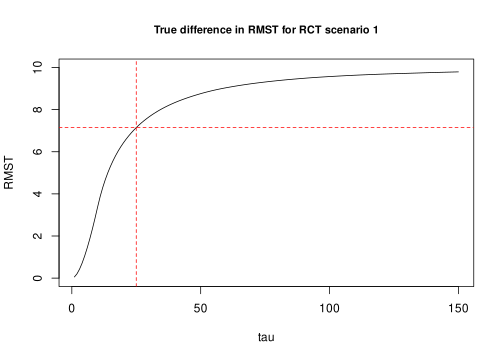
\includegraphics{Notebook_causal_survival_files/figure-pdf/unnamed-chunk-13-1.pdf}

\begin{verbatim}
[1] "The ground truth for RCT scenario 1 and 2 at time 25 is 7.1"
\end{verbatim}

\textbf{Estimation of the RMST}

For each Scenario, we estimate the difference in RMST using the methods
summarized in Section~\ref{sec-summary}. The methods used to estimate
the nuisance components are indicated in brackets: either logistic
regression or random forests for propensity scores and either cox models
or survival random forests for survival and censoring models. A naive
estimator where censored observations are simply removed and the
survival time is averaged for treated and controls is also provided for
a naive baseline.

Figure~\ref{fig-rct1} shows the distribution of the difference in RMST
for 100 simulations in Scenario 1 and different sample sizes: 500, 1000,
2000, 4000. The true value of \(\theta_{\mathrm{RMST}}\) is indicated by
red dotted line.

\begin{Shaded}
\begin{Highlighting}[]
\CommentTok{\# Update the theme to center the plot title}
\FunctionTok{theme\_update}\NormalTok{(}\AttributeTok{plot.title =} \FunctionTok{element\_text}\NormalTok{(}\AttributeTok{hjust =} \FloatTok{0.5}\NormalTok{))}

\CommentTok{\# Define the desired order of the estimators}

\NormalTok{desired\_order }\OtherTok{\textless{}{-}} \FunctionTok{c}\NormalTok{(}
  \StringTok{"Naive"}\NormalTok{,}
  \StringTok{"KM"}\NormalTok{,}
  \StringTok{"SurvRM2 {-} KM"}\NormalTok{,}
  \StringTok{"IPTW KM (Log. Reg.)"}\NormalTok{,}
  \StringTok{"RISCA {-} IPTW KM (Log. Reg.)"}\NormalTok{,}
  \StringTok{"IPCW KM (Cox)"}\NormalTok{,}
  \StringTok{"BJ (Cox)"}\NormalTok{,}
  \StringTok{"IPTW{-}BJ (Cox \& Log. Reg.)"}\NormalTok{,}
  \StringTok{"IPTW{-}IPCW KM (Cox \& Log. Reg.)"}\NormalTok{,}
  \StringTok{"G{-}formula (Cox/ T{-}learners)"}\NormalTok{,}
  \StringTok{"G{-}formula (Cox/ S{-}learner)"}\NormalTok{,}
  \StringTok{"RISCA {-} G\_formula (S{-}learner)"}\NormalTok{,}
  \StringTok{"AIPTW{-}AIPCW (Cox \& Cox \& Log. Reg.)"}\NormalTok{,}
  \StringTok{"grf {-} Causal Survival Forest"}\NormalTok{,}
  \StringTok{"IPTW KM (Forest)"}\NormalTok{,}
  \StringTok{"RISCA {-} IPTW KM (Forest)"}\NormalTok{,}
  \StringTok{"IPCW KM (Forest)"}\NormalTok{,}
  \StringTok{"BJ (Forest)"}\NormalTok{,}
  \StringTok{"IPTW{-}BJ (Forest)"}\NormalTok{,}
  \StringTok{"IPTW{-}IPCW KM (Forest)"}\NormalTok{,}
  \StringTok{"G{-}formula (Forest/ T{-}learners)"}\NormalTok{,}
  \StringTok{"G{-}formula (Forest/ S{-}learner)"}\NormalTok{,}
  \StringTok{"AIPTW{-}AIPCW (Forest)"}\NormalTok{)}

\CommentTok{\# Convert sample size to a factor with levels sorted in decreasing order}
\NormalTok{simulation\_rct1}\SpecialCharTok{$}\NormalTok{sample.size }\OtherTok{\textless{}{-}} \FunctionTok{factor}\NormalTok{(}
\NormalTok{  simulation\_rct1}\SpecialCharTok{$}\NormalTok{sample.size, }
  \AttributeTok{levels =} \FunctionTok{sort}\NormalTok{(}\FunctionTok{unique}\NormalTok{(simulation\_rct1}\SpecialCharTok{$}\NormalTok{sample.size), }\AttributeTok{decreasing =} \ConstantTok{FALSE}\NormalTok{)}
\NormalTok{)}

\CommentTok{\# Convert estimator column to a factor with the specified order}
\NormalTok{simulation\_rct1}\SpecialCharTok{$}\NormalTok{estimator }\OtherTok{\textless{}{-}} \FunctionTok{factor}\NormalTok{(simulation\_rct1}\SpecialCharTok{$}\NormalTok{estimator, }
                                    \AttributeTok{levels =}\NormalTok{ desired\_order)}

\CommentTok{\# Create the plot for RCT + independent censoring}
\NormalTok{simulation\_graph\_rct1 }\OtherTok{\textless{}{-}}\NormalTok{ simulation\_rct1 }\SpecialCharTok{\%\textgreater{}\%}
  \FunctionTok{ggplot}\NormalTok{(}\FunctionTok{aes}\NormalTok{(}
    \AttributeTok{x =}\NormalTok{ estimator, }\AttributeTok{y =}\NormalTok{ estimate,  }
    \AttributeTok{fill =} \FunctionTok{factor}\NormalTok{(sample.size, }\AttributeTok{levels =} \FunctionTok{rev}\NormalTok{(}\FunctionTok{levels}\NormalTok{(sample.size)))}
\NormalTok{  )) }\SpecialCharTok{+}
  \FunctionTok{scale\_fill\_brewer}\NormalTok{(}\AttributeTok{palette =} \StringTok{"Accent"}\NormalTok{) }\SpecialCharTok{+}
  \FunctionTok{geom\_boxplot}\NormalTok{(}\AttributeTok{alpha =} \FloatTok{0.9}\NormalTok{, }\AttributeTok{show.legend =} \ConstantTok{TRUE}\NormalTok{, }\AttributeTok{position =} \StringTok{"dodge"}\NormalTok{) }\SpecialCharTok{+}
  \FunctionTok{xlab}\NormalTok{(}\StringTok{""}\NormalTok{) }\SpecialCharTok{+}  \CommentTok{\# Change x{-}axis label}
  \FunctionTok{ylab}\NormalTok{(}\StringTok{"ATE"}\NormalTok{) }\SpecialCharTok{+}  \CommentTok{\# Change y{-}axis label}
  \FunctionTok{stat\_boxplot}\NormalTok{(}\AttributeTok{geom =} \StringTok{"errorbar"}\NormalTok{) }\SpecialCharTok{+}
  \FunctionTok{geom\_hline}\NormalTok{(}
    \AttributeTok{yintercept =}\NormalTok{ truth\_tau1, }\AttributeTok{linetype =} \StringTok{"dashed"}\NormalTok{, }\AttributeTok{color =} \StringTok{"red"}\NormalTok{, }
    \AttributeTok{alpha =} \FloatTok{0.8}\NormalTok{, }\AttributeTok{size =} \FloatTok{0.8}
\NormalTok{  ) }\SpecialCharTok{+}
\FunctionTok{theme}\NormalTok{(}
    \AttributeTok{legend.title =} \FunctionTok{element\_blank}\NormalTok{(), }\AttributeTok{legend.position =} \StringTok{"bottom"}\NormalTok{,}
    \AttributeTok{legend.box =} \StringTok{"vertical"}\NormalTok{, }\AttributeTok{legend.text =} \FunctionTok{element\_text}\NormalTok{(}\AttributeTok{size =} \DecValTok{18}\NormalTok{),}
    \AttributeTok{axis.text.x =} \FunctionTok{element\_text}\NormalTok{(}\AttributeTok{angle =} \DecValTok{35}\NormalTok{, }\AttributeTok{vjust =} \DecValTok{1}\NormalTok{, }\AttributeTok{hjust =} \DecValTok{1}\NormalTok{),  }
    \CommentTok{\# Adjust text angle for better visibility}
    \AttributeTok{axis.text =} \FunctionTok{element\_text}\NormalTok{(}\AttributeTok{size =} \DecValTok{15}\NormalTok{, }\AttributeTok{face =} \StringTok{"bold"}\NormalTok{),}
    \AttributeTok{axis.title.x =} \FunctionTok{element\_text}\NormalTok{(}\AttributeTok{size =} \DecValTok{16}\NormalTok{, }\AttributeTok{face =} \StringTok{"bold"}\NormalTok{),}
    \AttributeTok{plot.margin =} \FunctionTok{margin}\NormalTok{(}\AttributeTok{t =} \DecValTok{10}\NormalTok{, }\AttributeTok{r =} \DecValTok{10}\NormalTok{, }\AttributeTok{b =} \DecValTok{50}\NormalTok{, }\AttributeTok{l =} \DecValTok{10}\NormalTok{)  }\CommentTok{\# Add margin}
\NormalTok{  ) }\SpecialCharTok{+}    
  \FunctionTok{coord\_cartesian}\NormalTok{(}\AttributeTok{ylim =} \FunctionTok{c}\NormalTok{(}\DecValTok{0}\NormalTok{, }\DecValTok{15}\NormalTok{))}
\end{Highlighting}
\end{Shaded}

\begin{figure}

\centering{

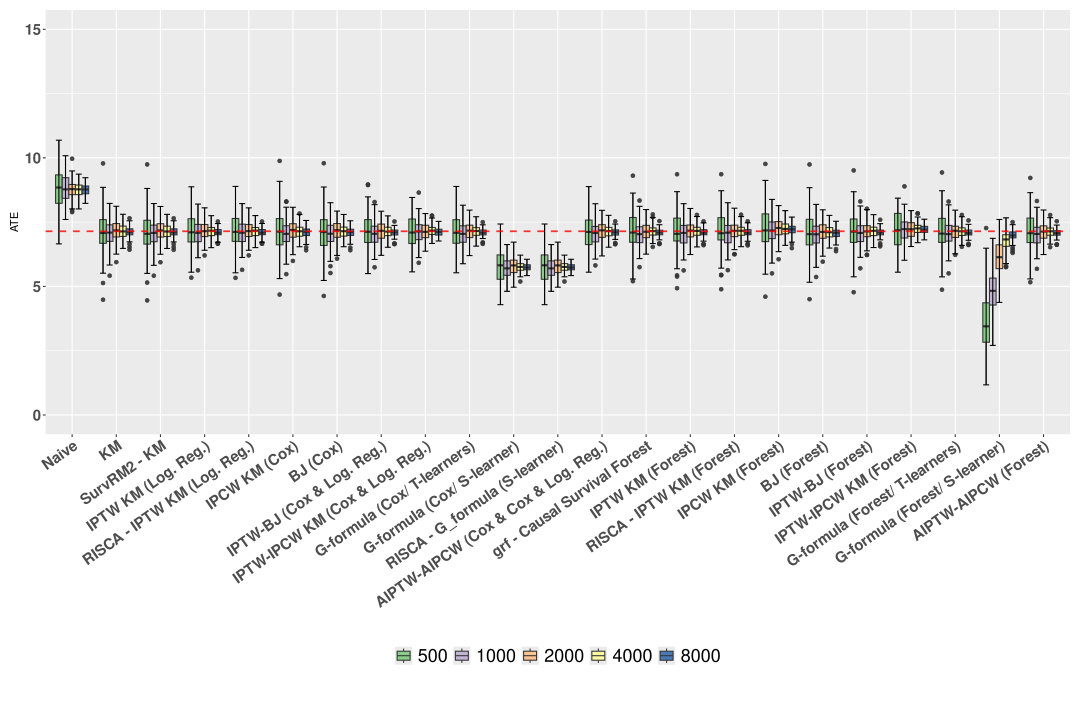
\includegraphics{Notebook_causal_survival_files/figure-pdf/fig-rct1-1.pdf}

}

\caption{\label{fig-rct1}Results of the ATE for the simulation of a RCT
with independent censoring.}

\end{figure}%

In this setting, and in accordance with the theory, the simplest
estimator (unadjusted KM) performs just as well as the others, and
presents an extremely small bias (as derived in
Section~\ref{sec-theoryRCT_indc}).

The naive estimator is biased, as expected, and the bias in both the
G-formula (RISCA) and the manual G-formula S-learner arises because the
treatment effect is additive \(T(1) = T(0) + 10\) and violates the
assumption that \(T\) would follow a Cox model in the variables
\((X,A)\). However, \(T|A=a\) is a Cox-model for \(a \in \{0,1\}\),
which explain the remarkable performance of G-formula (Cox/T-learners)
and some of the other models based on a Cox estimation of \(S\).

Other estimators (IPTW KM (Reg.Log), IPCW KM (Cox), IPTW-IPCW KM (Cox \&
Log.Reg), IPTW-BJ (Cox \& Log.Reg), AIPTW-AIPCW (Cox \& Cox \& Log.Reg))
involve unnecessary nuisance parameter estimates, such as propensity
scores or censoring models. Despite this, their performance remains
relatively stable in terms of variability, and there are roughly no
differences between using (semi-)parametric or non-parametric estimation
methods for nuisance parameters except for IPCW KM and IPTW-IPCW KM
where there is a slight bias when using forest-based methods.

\begin{figure}

\centering{

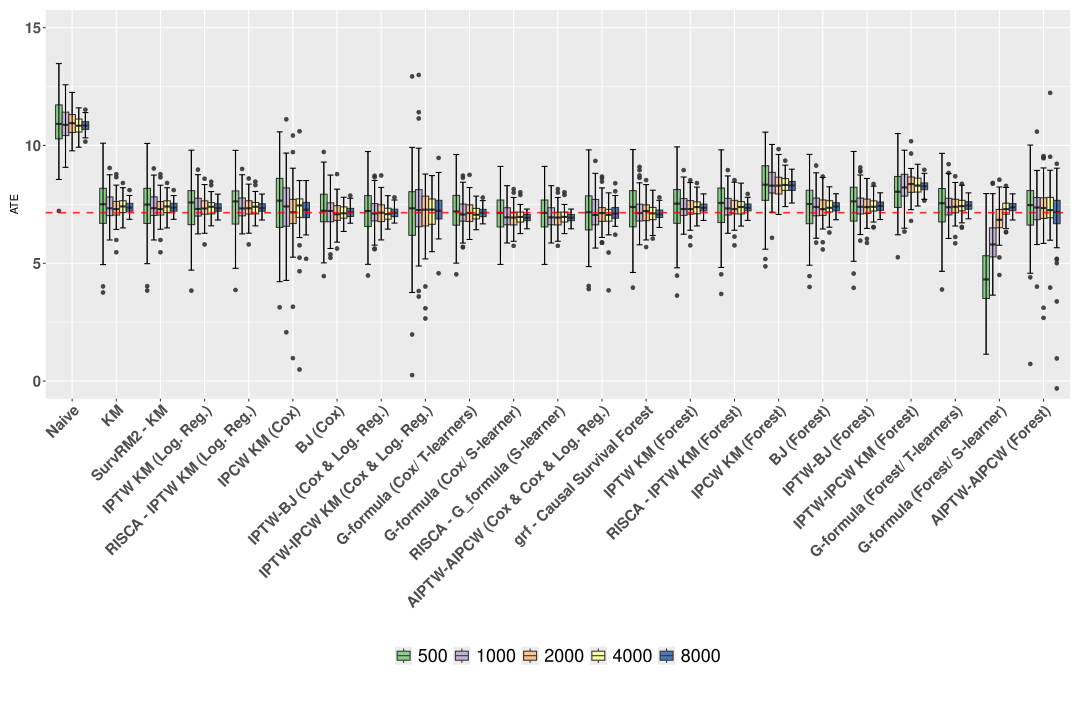
\includegraphics{Notebook_causal_survival_files/figure-pdf/fig-rct2-1.pdf}

}

\caption{\label{fig-rct2}Estimation results of the ATE for the
simulation of a RCT with dependent censoring.}

\end{figure}%

Figure~\ref{fig-rct2} shows the results for the RCT simulation with
conditionally independent censoring (Scenario 2). In this setting, the
Naive estimator remains biased. Similarly, both the unadjusted
Kaplan-Meier (KM) and its SurvRM2 equivalent, as well as the
treatment-adjusted IPTW KM and its RISCA equivalent, are biased due to
their failure to account for dependent censoring. As in Scenario 1,
G-formula (Cox/ S-learner) and its RISCA equivalent also remain biased.
The IPCW KM (Cox) is slightly biased up to 4,000 observations and quite
variable due to extreme censoring probabilities. IPTW-IPCW KM (Cox \&
Log.Reg.) is not biased but shows high variance. In contrast, the
Buckley-James estimator BJ (Cox) is unbiased even with as few as 500
observations. The BJ estimator also demonstrates smaller variance than
IPCW methods. G-formula (Cox/ T-learners) and AIPCW-AIPTW (Cox \& Cox \&
Log.Reg.) estimators seem to perform well, even in small samples. The
forest versions of these estimators seem more biased, except Causal
Survival Forest and the AIPTW-AIPCW (Forest). Notably, all estimators
exhibit higher variability compared to Scenario 1.

\subsection{Observational data}\label{sec-simulation-Obs}

\textbf{Data Generating Process}

As for Scenarii 1 and 2, we carry out two simulations of an
observational study with both independent and conditional independent
censoring. The only difference lies in the simulation of the propensity
score, which is no longer constant. For the simulation, an iid
\(n\)-sample \((X_{i},A_{i},C,T_{i}(0), T_{i}(1))_{i \in [n]}\) is
generated as in Section~\ref{sec-simulation-RCT}, except for the
treatment allocation process that is given by:

\[
\operatorname{logit}(e(X))= \beta_A^\top X \quad \text{where} \quad \beta_A = (-1,-1,-2.5,-1),
\]\\
where we recall that \(\operatorname{logit}(p) = \log(p/(1-p))\). The
descriptive statistics for the two observational data with independent
(\(\texttt{Obs1}\)) and conditionally independent censoring
(\(\texttt{Obs2}\)) are displayed in Appendix
(Section~\ref{sec-stat_obs}). Note that we did not modify the survival
distribution, the target difference in RMST is thus the same.

\begin{Shaded}
\begin{Highlighting}[]
\CommentTok{\# Obs1:  Treatment assignment dependent on X + independent censoring}
\CommentTok{\# Obs2:  Treatment assignment dependent on X + dependent censoring (conditional }
\CommentTok{\# on X)}

\CommentTok{\# Function to simulate observational data for two scenarios: Obs1 and Obs2}
\NormalTok{simulate\_data\_obs }\OtherTok{\textless{}{-}} \ControlFlowTok{function}\NormalTok{(n, }
                              \AttributeTok{mu =} \FunctionTok{c}\NormalTok{(}\DecValTok{1}\NormalTok{, }\DecValTok{1}\NormalTok{, }\SpecialCharTok{{-}}\DecValTok{1}\NormalTok{, }\DecValTok{1}\NormalTok{), }
                              \AttributeTok{sigma =} \FunctionTok{diag}\NormalTok{(}\DecValTok{4}\NormalTok{), }
                              \AttributeTok{colnames\_cov =} \FunctionTok{c}\NormalTok{(}\StringTok{"X1"}\NormalTok{, }\StringTok{"X2"}\NormalTok{, }\StringTok{"X3"}\NormalTok{, }\StringTok{"X4"}\NormalTok{),}
\NormalTok{                              tau,}
                              \AttributeTok{coefT0 =} \FloatTok{0.01}\NormalTok{, }
                              \AttributeTok{parsS =} \FunctionTok{c}\NormalTok{(}\FloatTok{0.5}\NormalTok{, }\FloatTok{0.5}\NormalTok{, }\SpecialCharTok{{-}}\FloatTok{0.5}\NormalTok{, }\FloatTok{0.5}\NormalTok{),}
                              \AttributeTok{parsA =} \FunctionTok{c}\NormalTok{(}\SpecialCharTok{{-}}\DecValTok{1}\NormalTok{, }\SpecialCharTok{{-}}\DecValTok{1}\NormalTok{, }\SpecialCharTok{{-}}\FloatTok{2.5}\NormalTok{, }\SpecialCharTok{{-}}\DecValTok{1}\NormalTok{), }
                              \AttributeTok{parsC\_A =} \FunctionTok{c}\NormalTok{(}\DecValTok{0}\NormalTok{), }
                              \AttributeTok{coefC =} \FloatTok{0.03}\NormalTok{,}
                              \AttributeTok{parsC =} \FunctionTok{c}\NormalTok{(}\FloatTok{0.7}\NormalTok{, }\FloatTok{0.3}\NormalTok{, }\SpecialCharTok{{-}}\FloatTok{0.25}\NormalTok{, }\SpecialCharTok{{-}}\FloatTok{0.1}\NormalTok{), }
                              \AttributeTok{scenario =} \StringTok{"Obs2"}\NormalTok{) \{}
  
  \CommentTok{\# Generate covariates X from a multivariate normal distribution}
\NormalTok{  X }\OtherTok{\textless{}{-}} \FunctionTok{mvrnorm}\NormalTok{(n, mu, sigma)}
\NormalTok{  X }\OtherTok{\textless{}{-}} \FunctionTok{as.data.frame}\NormalTok{(X)}
  \FunctionTok{colnames}\NormalTok{(X) }\OtherTok{\textless{}{-}}\NormalTok{ colnames\_cov}
  
  \CommentTok{\# Propensity score model based on X}
\NormalTok{  e }\OtherTok{\textless{}{-}} \FunctionTok{rowSums}\NormalTok{(}\FunctionTok{as.matrix}\NormalTok{(X) }\SpecialCharTok{\%*\%} \FunctionTok{diag}\NormalTok{(parsA))}
\NormalTok{  e }\OtherTok{\textless{}{-}} \FunctionTok{plogis}\NormalTok{(e)  }\CommentTok{\# Transform to probability scale}
  
  \CommentTok{\# Treatment assignment based on the propensity score}
\NormalTok{  A }\OtherTok{\textless{}{-}} \FunctionTok{sapply}\NormalTok{(e, }\AttributeTok{FUN =} \ControlFlowTok{function}\NormalTok{(p) }\FunctionTok{rbinom}\NormalTok{(}\AttributeTok{n =} \DecValTok{1}\NormalTok{, }\AttributeTok{size =} \DecValTok{1}\NormalTok{, }\AttributeTok{prob =}\NormalTok{ p))}
  
  \CommentTok{\# Outcome model based on X}
\NormalTok{  X\_outcome }\OtherTok{\textless{}{-}} \FunctionTok{as.matrix}\NormalTok{(X)}
\NormalTok{  epsilon }\OtherTok{\textless{}{-}} \FunctionTok{runif}\NormalTok{(n, }\AttributeTok{min =} \FloatTok{0.00000001}\NormalTok{, }\AttributeTok{max =} \DecValTok{1}\NormalTok{)}
\NormalTok{  T0 }\OtherTok{\textless{}{-}} \SpecialCharTok{{-}}\FunctionTok{log}\NormalTok{(epsilon) }\SpecialCharTok{/}\NormalTok{ (coefT0 }\SpecialCharTok{*} \FunctionTok{exp}\NormalTok{(X\_outcome }\SpecialCharTok{\%*\%}\NormalTok{ parsS))}
  
  \CommentTok{\# Define treatment effect (shift in survival time due to treatment)}
\NormalTok{  T1 }\OtherTok{\textless{}{-}}\NormalTok{ T0 }\SpecialCharTok{+} \DecValTok{10}
  
  \ControlFlowTok{if}\NormalTok{ (scenario }\SpecialCharTok{==} \StringTok{"Obs1"}\NormalTok{) \{}
    \CommentTok{\# Scenario 1: Independent censoring}
\NormalTok{    C }\OtherTok{\textless{}{-}} \SpecialCharTok{{-}}\FunctionTok{log}\NormalTok{(}\FunctionTok{runif}\NormalTok{(n, }\AttributeTok{min =} \FloatTok{0.00000001}\NormalTok{, }\AttributeTok{max =} \DecValTok{1}\NormalTok{)) }\SpecialCharTok{/}\NormalTok{ coefC}
    
\NormalTok{  \} }\ControlFlowTok{else} \ControlFlowTok{if}\NormalTok{ (scenario }\SpecialCharTok{==} \StringTok{"Obs2"}\NormalTok{) \{}
    \CommentTok{\# Scenario 2: Dependent censoring based on X}
\NormalTok{    X\_censoring }\OtherTok{\textless{}{-}} \FunctionTok{as.matrix}\NormalTok{(}\FunctionTok{cbind}\NormalTok{(X,A))}
\NormalTok{    parsC }\OtherTok{\textless{}{-}} \FunctionTok{c}\NormalTok{(parsC,parsC\_A)}
    
\NormalTok{    C }\OtherTok{\textless{}{-}} \SpecialCharTok{{-}}\FunctionTok{log}\NormalTok{(}\FunctionTok{runif}\NormalTok{(n, }\AttributeTok{min =} \FloatTok{0.00000001}\NormalTok{, }\AttributeTok{max =} \DecValTok{1}\NormalTok{)) }\SpecialCharTok{/} 
\NormalTok{      (coefC }\SpecialCharTok{*} \FunctionTok{exp}\NormalTok{(}\FunctionTok{rowSums}\NormalTok{(X\_censoring }\SpecialCharTok{\%*\%} \FunctionTok{diag}\NormalTok{(parsC))))}
    
\NormalTok{  \} }\ControlFlowTok{else}\NormalTok{ \{}
    \FunctionTok{stop}\NormalTok{(}\StringTok{"Invalid scenario. Choose \textquotesingle{}Obs1\textquotesingle{} or \textquotesingle{}Obs2\textquotesingle{}."}\NormalTok{)}
\NormalTok{  \}}
  
  \CommentTok{\# Determine the true survival time based on treatment}
\NormalTok{  T\_true }\OtherTok{\textless{}{-}}\NormalTok{ A }\SpecialCharTok{*}\NormalTok{ T1 }\SpecialCharTok{+}\NormalTok{ (}\DecValTok{1} \SpecialCharTok{{-}}\NormalTok{ A) }\SpecialCharTok{*}\NormalTok{ T0}
  
  \CommentTok{\# Observed time is the minimum of the true survival time and censoring time}
\NormalTok{  T\_obs }\OtherTok{\textless{}{-}} \FunctionTok{pmin}\NormalTok{(T\_true, C)}
  
  \CommentTok{\# Status indicator: 1 if the event (death) occurred, 0 if censored}
\NormalTok{  status }\OtherTok{\textless{}{-}} \FunctionTok{as.numeric}\NormalTok{(T\_true }\SpecialCharTok{\textless{}=}\NormalTok{ C)}
  
  \CommentTok{\# Restricted survival time (censored at tau)}
\NormalTok{  T\_obs\_tau }\OtherTok{\textless{}{-}} \FunctionTok{pmin}\NormalTok{(T\_obs, tau)}
\NormalTok{  status\_tau }\OtherTok{\textless{}{-}} \FunctionTok{as.numeric}\NormalTok{((T\_obs }\SpecialCharTok{\textgreater{}}\NormalTok{ tau) }\SpecialCharTok{|}\NormalTok{ (T\_obs }\SpecialCharTok{\textless{}=}\NormalTok{ tau }\SpecialCharTok{\&}\NormalTok{ status }\SpecialCharTok{==} \DecValTok{1}\NormalTok{))}
  
  \CommentTok{\# Compile the simulated data into a data frame}
\NormalTok{  DATA\_target\_population }\OtherTok{\textless{}{-}} \FunctionTok{data.frame}\NormalTok{(X, tau, A, T0, T1, C, T\_obs, T\_obs\_tau, }
\NormalTok{                                       status, status\_tau, e)}
  
  \FunctionTok{return}\NormalTok{(DATA\_target\_population)}
\NormalTok{\}}
\end{Highlighting}
\end{Shaded}

\begin{verbatim}
[1] "The ground truth for Obs scenario 1 at time 25 is 7.1"
\end{verbatim}

\begin{verbatim}
[1] "The ground truth for Obs scenario 2 at #time 25 is 7.1"
\end{verbatim}

\textbf{Estimation of the RMST}

Figure~\ref{fig-obs1} below shows the distribution of the estimators of
\(\theta_{\mathrm{RMST}}\) for the observational study with independent
censoring.

\begin{figure}

\centering{

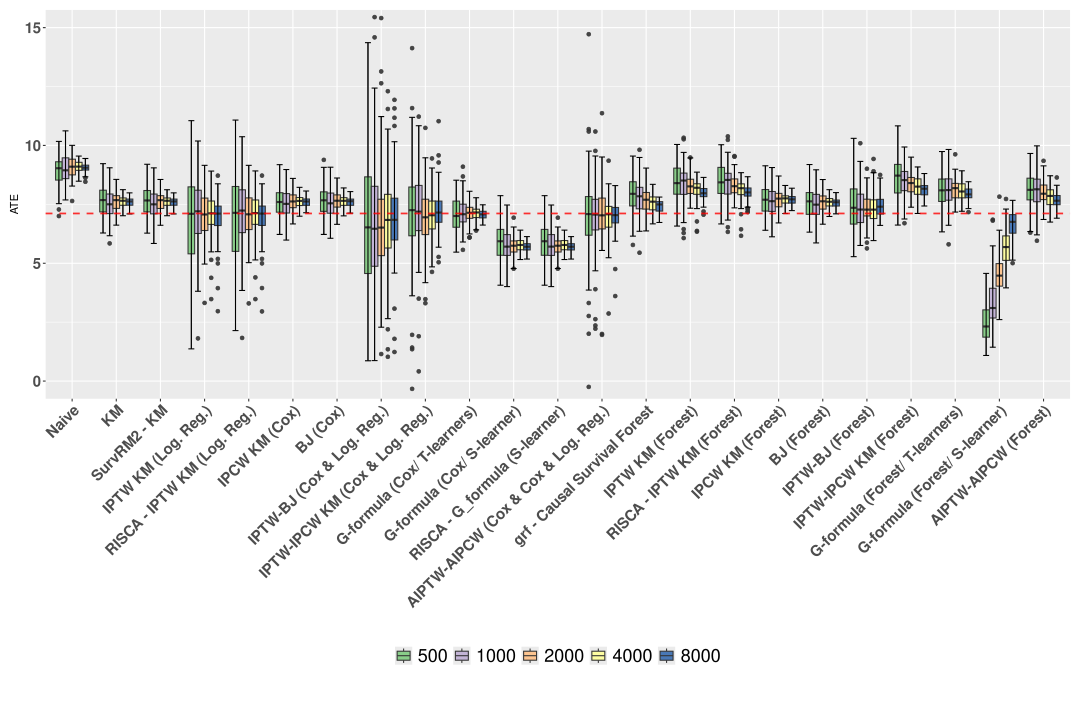
\includegraphics{Notebook_causal_survival_files/figure-pdf/fig-obs1-1.pdf}

}

\caption{\label{fig-obs1}Estimation results of the ATE for the
simulation of an observational study with independent censoring.}

\end{figure}%

In the simulation of an observational study with independent censoring,
confounding bias is introduced, setting it apart from RCT simulations.
As expected, estimators that fail to adjust for this bias, such as
unadjusted Kaplan-Meier (KM), IPCW KM (Cox), and their equivalents, are
biased. However, estimators like IPTW KM (Log.Reg.), IPTW-IPCW KM (Cox
\& Log. Reg.) are unbiased, even if the latter estimate unnecessary
nuisance components. Results with IPTW BJ (Cox \& Log.Reg) are extremely
variable.

The top-performing estimators in this scenario are G-formula (Cox/
T-learners) and AIPCW-AIPTW (Cox \& Cox \& Log.Reg.), which are unbiased
even with 500 observations. The former has the lowest variance. All
estimators that use forests to estimate nuisance parameters are biased
across sample sizes from 500 to 8000. Although Causal Survival Forest
and AIPW-AIPCW (Forest) are expected to eventually converge, they remain
extremely demanding in terms of sample size. This setting thus
highlights that one should either have an a priori knowledge on the
specification of the models or large sample size.

Figure~\ref{fig-obs2} below shows the distribution of the
\(\theta_{\mathrm{RMST}}\) estimates for the observational study with
conditionally independent censoring. The red dashed line represents the
true \(\theta_{\mathrm{RMST}}\) for \(\tau=25\).

\begin{figure}

\centering{

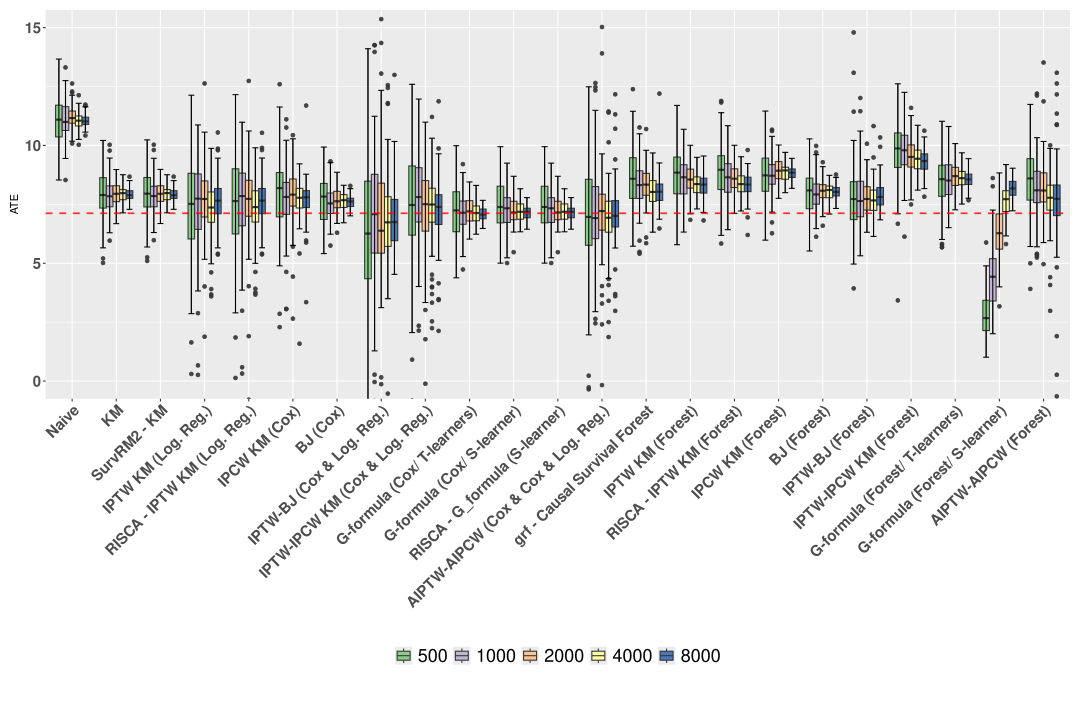
\includegraphics{Notebook_causal_survival_files/figure-pdf/fig-obs2-1.pdf}

}

\caption{\label{fig-obs2}Estimation results of the ATE for the
simulation of an observational study with dependent censoring.}

\end{figure}%

In the simulation of an observational study with conditionally
independent censoring, estimators that do not account for both censoring
and confounding bias, such as KM, IPCW KM, IPTW KM, and their package
equivalents, are biased. The top-performing estimators in this scenario
are G-formula (Cox/ T-learners) and AIPCW-AIPTW (Cox \& Cox \&
Log.Reg.), which are unbiased even with 500 observations. The former has
the lowest variance as expected, see Section~\ref{sec-Gformula}.
Surprisingly, the G-formula (Cox/S-learner) and its equivalent from the
RISCA package perform quite competitively, showing only a slight bias
despite the violation of the proportional hazards assumption. All
estimators that use forests to estimate nuisance parameters are biased
across sample sizes from 500 to 8000. Although Causal Survival Forest
and AIPTW-AIPCW (Forest) are expected to eventually converge, they
remain extremely demanding in terms of sample size.

\subsection{Mispecification of nuisance
components}\label{mispecification-of-nuisance-components}

\textbf{Data Generating Process}

We generate an observational study with covariate interactions and
conditionally independent censoring. The objective is to assess the
impact of misspecifying nuisance components; specifically, we will use
models that omit interactions to estimate these components. This
approach enables us to evaluate the robustness properties of various
estimators. In addition, in this setting forest based methods are
expected to behave better.

We generate \(n\) samples \((X_{i},A_{i},C,T_{i}(0), T_{i}(1))\) as
follows:

\begin{itemize}
\item
  \(X \sim \mathcal{N}\left(\mu, \Sigma\right)\) and
  \(\mu = (0.5,0.5,0.7,0.5)\), \(\Sigma = \mathrm{Id}_4\).
\item
  The hazard function of \(T(0)\) is given by \[
  \begin{aligned}
  \lambda^{(0)}(t|X) = \exp\{\beta_0^\top Y\} \quad \text{where} \quad \beta_0 &= (0.2,0.3,0.1,0.1,1,0,0,0,0,1), \\
  \text{and} \quad Y &= (X_1^2,X_2^2,X_3^2,X_4^2,X_1 X_2,X_1X_3,X_1X_4,X_2 X_3,X_2X_4, X_3 X_4).
  \end{aligned}
  \]
\item
  The distribution of \(T(1)\) is the one of \(T(0)\) but shifted:
  \(T(1) = T(0)+1\).
\item
  The hazard function of \(C\) is given by \[
  \begin{aligned}
  \lambda_C(t|X) = \exp\{\beta_C^\top Y\} \quad \text{where} \quad \beta_C &= (0.05,0.05,-0.1,0.1,0,1,0,-1,0,0).
  \end{aligned}
  \]
\item
  The propensity score is \[
  \begin{aligned}
  \mathrm{logit}(e(x)) = \beta_A^\top Y \quad \text{where} \quad \beta_A= (0.05,-0.1,0.5,-0.1,1,0,1,0,0,0).
  \end{aligned}
  \] When the model is well-specified, the full vector \((X,Y)\) is
  given as an input of the nuisance parameter models. When it is not,
  only \(X\) and the first half of \(Y\) corresponding to
  \((X_1^2,X_2^2,X_3^2,X_4^2)\) is given as an input.
\end{itemize}

\begin{Shaded}
\begin{Highlighting}[]
\CommentTok{\# DGP for misspecification }
\NormalTok{simulate\_data\_mis }\OtherTok{\textless{}{-}} \ControlFlowTok{function}\NormalTok{(n, }
                              \AttributeTok{mu =} \FunctionTok{c}\NormalTok{(}\FloatTok{0.5}\NormalTok{, }\FloatTok{0.5}\NormalTok{, }\FloatTok{0.7}\NormalTok{, }\FloatTok{0.5}\NormalTok{),}
                              \AttributeTok{sigma =}  \FunctionTok{matrix}\NormalTok{(}\FunctionTok{c}\NormalTok{(}\DecValTok{1}\NormalTok{, }\DecValTok{0}\NormalTok{, }\DecValTok{0}\NormalTok{, }\DecValTok{0}\NormalTok{, }
                                                \DecValTok{0}\NormalTok{, }\DecValTok{1}\NormalTok{, }\DecValTok{0}\NormalTok{, }\DecValTok{0}\NormalTok{, }
                                                \DecValTok{0}\NormalTok{, }\DecValTok{0}\NormalTok{, }\DecValTok{1}\NormalTok{, }\DecValTok{0}\NormalTok{,}
                                                \DecValTok{0}\NormalTok{, }\DecValTok{0}\NormalTok{, }\DecValTok{0}\NormalTok{, }\DecValTok{1}\NormalTok{), }
                                              \AttributeTok{nrow =} \DecValTok{4}\NormalTok{, }\AttributeTok{byrow =} \ConstantTok{TRUE}\NormalTok{),}
                              \AttributeTok{colnames\_cov =} \FunctionTok{c}\NormalTok{(}\StringTok{"X1"}\NormalTok{, }\StringTok{"X2"}\NormalTok{, }\StringTok{"X3"}\NormalTok{, }\StringTok{"X4"}\NormalTok{),}
                              \AttributeTok{parsA =}  \FunctionTok{c}\NormalTok{(}\FloatTok{0.05}\NormalTok{, }\SpecialCharTok{{-}}\FloatTok{0.1}\NormalTok{, }\FloatTok{0.5}\NormalTok{, }\SpecialCharTok{{-}}\FloatTok{0.1}\NormalTok{),}
\NormalTok{                              tau)\{}
  
  \CommentTok{\# Generate X from a multivariate normal distribution}
\NormalTok{  X }\OtherTok{\textless{}{-}}\NormalTok{ MASS}\SpecialCharTok{::}\FunctionTok{mvrnorm}\NormalTok{(n, mu, sigma)}
\NormalTok{  X }\OtherTok{\textless{}{-}} \FunctionTok{as.data.frame}\NormalTok{(X)}
  \FunctionTok{colnames}\NormalTok{(X) }\OtherTok{\textless{}{-}}\NormalTok{ colnames\_cov}
  
  \CommentTok{\# Treatment variable selection: all X}
\NormalTok{  X\_treatment }\OtherTok{\textless{}{-}} \FunctionTok{as.matrix}\NormalTok{(X)}
  
  \CommentTok{\# Propensity score model based on X}
\NormalTok{  e }\OtherTok{\textless{}{-}}\NormalTok{ parsA[}\DecValTok{1}\NormalTok{]}\SpecialCharTok{*}\NormalTok{X\_treatment[, }\StringTok{"X1"}\NormalTok{]}\SpecialCharTok{\^{}}\DecValTok{2} \SpecialCharTok{+}\NormalTok{ parsA[}\DecValTok{2}\NormalTok{]}\SpecialCharTok{*}\NormalTok{X\_treatment[, }\StringTok{"X2"}\NormalTok{]}\SpecialCharTok{\^{}}\DecValTok{2} \SpecialCharTok{+} 
\NormalTok{    parsA[}\DecValTok{3}\NormalTok{]}\SpecialCharTok{*}\NormalTok{X\_treatment[, }\StringTok{"X3"}\NormalTok{]}\SpecialCharTok{\^{}}\DecValTok{2} \SpecialCharTok{+}\NormalTok{ parsA[}\DecValTok{4}\NormalTok{]}\SpecialCharTok{*}\NormalTok{X\_treatment[, }\StringTok{"X4"}\NormalTok{]}\SpecialCharTok{\^{}}\DecValTok{2}\SpecialCharTok{{-}}
\NormalTok{    X\_treatment[, }\StringTok{"X1"}\NormalTok{]}\SpecialCharTok{*}\NormalTok{X\_treatment[, }\StringTok{"X2"}\NormalTok{] }\SpecialCharTok{+}
\NormalTok{    X\_treatment[, }\StringTok{"X1"}\NormalTok{]}\SpecialCharTok{*}\NormalTok{X\_treatment[, }\StringTok{"X4"}\NormalTok{]}
  
  \CommentTok{\# Logistic regression}
\NormalTok{  e }\OtherTok{\textless{}{-}} \FunctionTok{plogis}\NormalTok{(e)}
  
  \CommentTok{\# Treatment assignment based on the propensity score}
\NormalTok{  A }\OtherTok{\textless{}{-}} \FunctionTok{sapply}\NormalTok{(e, }\AttributeTok{FUN =} \ControlFlowTok{function}\NormalTok{(p) }\FunctionTok{rbinom}\NormalTok{(}\AttributeTok{n =} \DecValTok{1}\NormalTok{, }\AttributeTok{size =} \DecValTok{1}\NormalTok{, }\AttributeTok{prob =}\NormalTok{ p))}
  
  \CommentTok{\# Outcome variable selection: all X}
\NormalTok{  X\_outcome }\OtherTok{\textless{}{-}} \FunctionTok{as.matrix}\NormalTok{(X)}
  
\NormalTok{  lambda }\OtherTok{\textless{}{-}} \FunctionTok{exp}\NormalTok{(}\FloatTok{0.2}\SpecialCharTok{*}\NormalTok{X[,}\DecValTok{1}\NormalTok{]}\SpecialCharTok{\^{}}\DecValTok{2} \SpecialCharTok{+} \FloatTok{0.3}\SpecialCharTok{*}\NormalTok{X[,}\DecValTok{2}\NormalTok{]}\SpecialCharTok{\^{}}\DecValTok{2} \SpecialCharTok{+} \FloatTok{0.1}\SpecialCharTok{*}\NormalTok{X[,}\DecValTok{3}\NormalTok{]}\SpecialCharTok{\^{}}\DecValTok{2} \SpecialCharTok{+} \FloatTok{0.1}\SpecialCharTok{*}\NormalTok{X[,}\DecValTok{4}\NormalTok{]}\SpecialCharTok{\^{}}\DecValTok{2} \SpecialCharTok{+} 
\NormalTok{    X[,}\DecValTok{1}\NormalTok{] }\SpecialCharTok{*}\NormalTok{ X[,}\DecValTok{2}\NormalTok{] }\SpecialCharTok{+}\NormalTok{ X[,}\DecValTok{3}\NormalTok{] }\SpecialCharTok{*}\NormalTok{ X[,}\DecValTok{4}\NormalTok{])}
  \CommentTok{\# Simulate the outcome using the cumulative hazard inversion method}
\NormalTok{  epsilon }\OtherTok{\textless{}{-}} \FunctionTok{runif}\NormalTok{(n, }\AttributeTok{min =} \FloatTok{1e{-}8}\NormalTok{, }\AttributeTok{max =} \DecValTok{1}\NormalTok{)}
\NormalTok{  T0 }\OtherTok{\textless{}{-}} \SpecialCharTok{{-}}\FunctionTok{log}\NormalTok{(epsilon) }\SpecialCharTok{/}\NormalTok{ lambda}
  
  \CommentTok{\# Simulate independent censoring time}
\NormalTok{  censoring\_lambda }\OtherTok{\textless{}{-}} \FunctionTok{exp}\NormalTok{(}\FloatTok{0.05}\SpecialCharTok{*}\NormalTok{X[,}\DecValTok{1}\NormalTok{]}\SpecialCharTok{\^{}}\DecValTok{2} \SpecialCharTok{+} \FloatTok{0.05}\SpecialCharTok{*}\NormalTok{X[,}\DecValTok{2}\NormalTok{]}\SpecialCharTok{\^{}}\DecValTok{2}\FloatTok{{-}0.1}\SpecialCharTok{*}\NormalTok{X[,}\DecValTok{3}\NormalTok{]}\SpecialCharTok{\^{}}\DecValTok{2} \SpecialCharTok{+} \FloatTok{0.1}\SpecialCharTok{*}\NormalTok{X[,}\DecValTok{4}\NormalTok{]}\SpecialCharTok{\^{}}\DecValTok{2} \SpecialCharTok{+} 
\NormalTok{    X[,}\DecValTok{3}\NormalTok{] }\SpecialCharTok{*}\NormalTok{ X[,}\DecValTok{1}\NormalTok{] }\SpecialCharTok{{-}}\NormalTok{ X[,}\DecValTok{2}\NormalTok{]}\SpecialCharTok{*}\NormalTok{X[,}\DecValTok{4}\NormalTok{])}
\NormalTok{  epsilon }\OtherTok{\textless{}{-}} \FunctionTok{runif}\NormalTok{(n, }\AttributeTok{min =} \FloatTok{1e{-}8}\NormalTok{, }\AttributeTok{max =} \DecValTok{1}\NormalTok{)}
\NormalTok{  C }\OtherTok{\textless{}{-}} \SpecialCharTok{{-}}\FunctionTok{log}\NormalTok{(epsilon) }\SpecialCharTok{/}\NormalTok{ censoring\_lambda}
  
  
  \CommentTok{\# T(1) = T(0) + 1}
\NormalTok{  T1 }\OtherTok{\textless{}{-}}\NormalTok{ T0 }\SpecialCharTok{+} \DecValTok{1}
  
  \CommentTok{\# True survival time}
\NormalTok{  T\_true }\OtherTok{\textless{}{-}}\NormalTok{ A }\SpecialCharTok{*}\NormalTok{ T1 }\SpecialCharTok{+}\NormalTok{ (}\DecValTok{1} \SpecialCharTok{{-}}\NormalTok{ A) }\SpecialCharTok{*}\NormalTok{ T0}
  
  \CommentTok{\# Observed time}
\NormalTok{  T\_obs }\OtherTok{\textless{}{-}} \FunctionTok{pmin}\NormalTok{(T\_true, C)}
  
  \CommentTok{\# Status indicator}
\NormalTok{  status }\OtherTok{\textless{}{-}} \FunctionTok{as.numeric}\NormalTok{(T\_true }\SpecialCharTok{\textless{}=}\NormalTok{ C)}
\NormalTok{  censor.status }\OtherTok{\textless{}{-}} \FunctionTok{as.numeric}\NormalTok{(T\_true }\SpecialCharTok{\textgreater{}}\NormalTok{ C)}
  
  \CommentTok{\# Restricted survival time}
\NormalTok{  T\_obs\_tau }\OtherTok{\textless{}{-}} \FunctionTok{pmin}\NormalTok{(T\_obs, tau)}
\NormalTok{  status\_tau }\OtherTok{\textless{}{-}} \FunctionTok{as.numeric}\NormalTok{((T\_obs }\SpecialCharTok{\textgreater{}}\NormalTok{ tau) }\SpecialCharTok{|}\NormalTok{ (T\_obs }\SpecialCharTok{\textless{}=}\NormalTok{ tau }\SpecialCharTok{\&}\NormalTok{ status }\SpecialCharTok{==} \DecValTok{1}\NormalTok{))}
  \CommentTok{\# Compile the simulated data into a data frame}
\NormalTok{  DATA\_target\_population }\OtherTok{\textless{}{-}} \FunctionTok{data.frame}\NormalTok{(X, tau, A, T0, T1, C, T\_obs, T\_obs\_tau, }
\NormalTok{                                       status, status\_tau, censor.status, e)}
  
  \FunctionTok{return}\NormalTok{(DATA\_target\_population)}
\NormalTok{\}}
\end{Highlighting}
\end{Shaded}

The descriptive statistics are given in Appendix
(Section~\ref{sec-stat_inter}).

\begin{verbatim}
[1] "The ground truth for mis scenario at time 0.45 is 0.26"
\end{verbatim}

\textbf{Estimation of the RMST}

First, we estimate \(\theta_{\mathrm{RMST}}\) without any model
misspecification to confirm the consistency of the estimators under
correctly specified nuisance models. More specifically, it means that
for parametric propensity score models, semi-parametric censoring and
survival models, we use models including interactions and squared
assuming knowledge on the data generating process.

Next, we introduce misspecification individually for the treatment
model, censoring model, and outcome model (Figure~\ref{fig-mis}), i.e.,
we use models without interaction to estimate parametric and
semi-parametric nuisance components while the data are generated with
interactions.\\
We further examine combined misspecifications for pairs of models:
treatment and censoring, treatment and outcome, and outcome and
censoring. Finally, we assess the impact of misspecifying all nuisance
models simultaneously (Figure~\ref{fig-mis2}).

\begin{figure}

\centering{

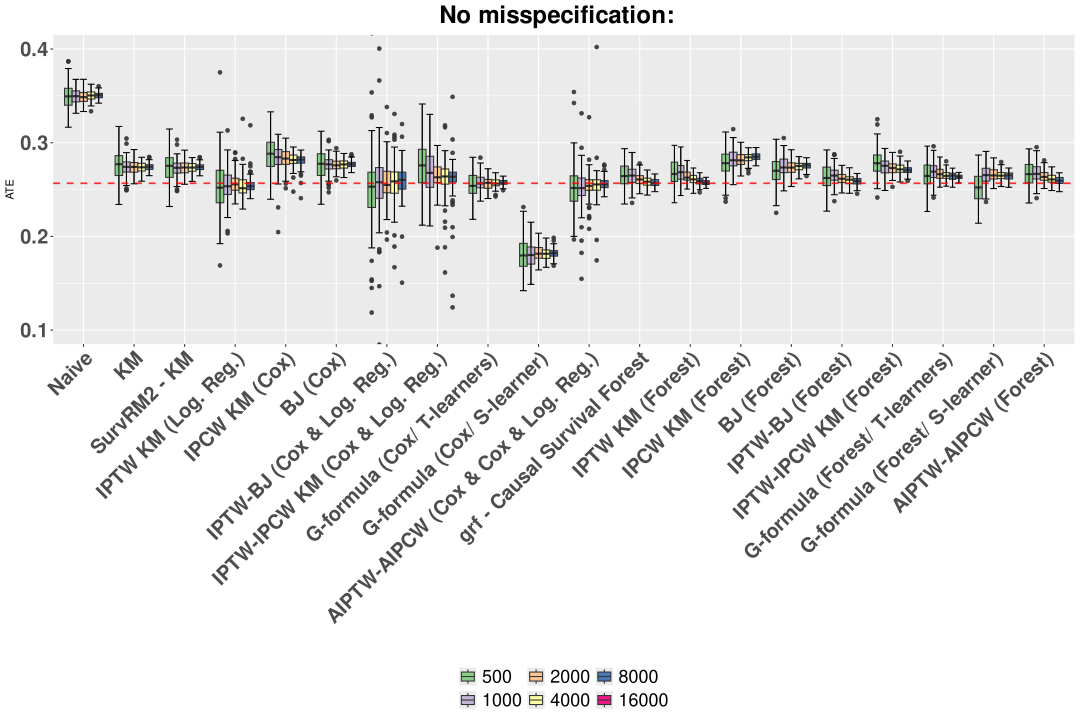
\includegraphics{Notebook_causal_survival_files/figure-pdf/fig-mis3-1.pdf}

}

\caption{\label{fig-mis3}Estimation results of the ATE for the
simulation of an observational study with dependent censoring and non
linear relationships.}

\end{figure}%

\begin{figure}

\centering{

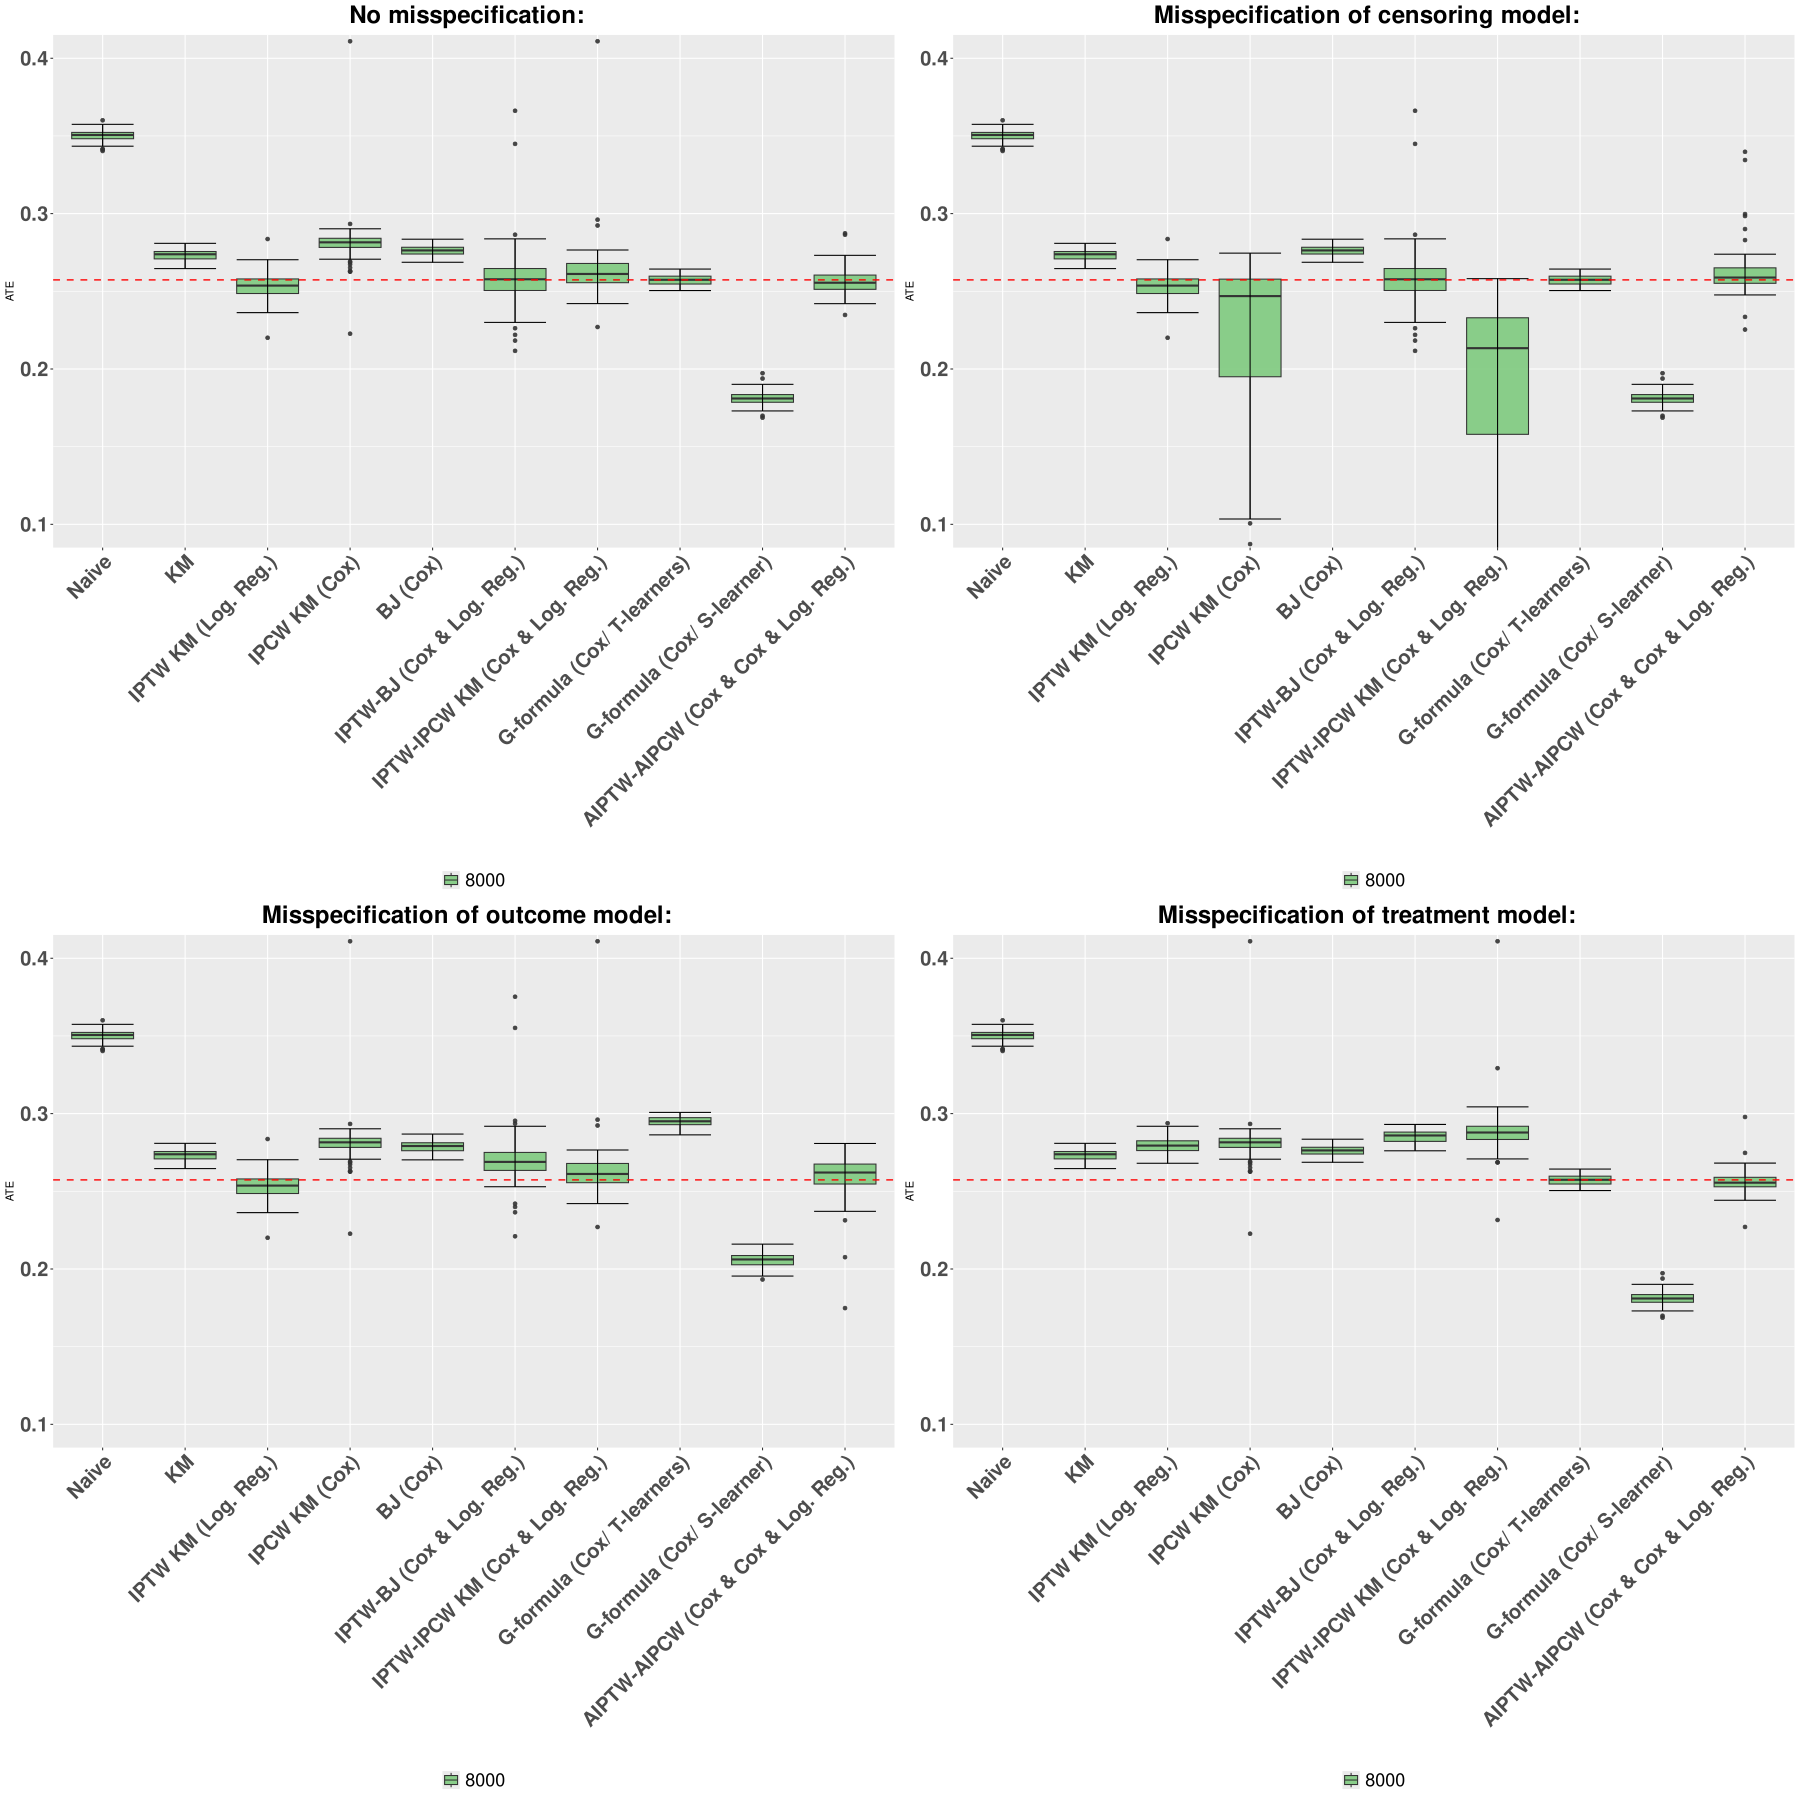
\includegraphics{Notebook_causal_survival_files/figure-pdf/fig-mis-1.pdf}

}

\caption{\label{fig-mis}Estimation results of the ATE for an
observational study with dependent censoring in case of a single
misspecification.}

\end{figure}%

When there is no misspecification in Figure~\ref{fig-mis3}, as expected,
IPTW-BJ (Cox \& Log.Reg), G-formula (Cox/ T-learners) and AIPTW-AIPCW
(Cox \& Cox \& Reg.Log) are unbiased. IPTW-IPCW KM (Cox \& Log.Reg)
exhibits a bias but seems to converge at larger sample size. Regarding
forest-based methods, IPTW-BJ (Forest), AIPTW-AIPCW (Forest) and Causal
Survival Forest estimate accurately the difference in RMST.
Surprisingly, G-formula (Forest/ T-learners), G-formula (Forest/
S-learner) and IPTW-IPCW KM (Forest) exhibit small bias but are expected
to eventually converge at large sample size.

Figure~\ref{fig-mis} shows that AIPTW-AIPCW (Cox \& Cox \& Reg.Log) is
convergent when there is one nuisance misspecification. In contrary, the
other estimators are biased when one of its nuisance parameter is
misspecified.

\begin{figure}

\centering{

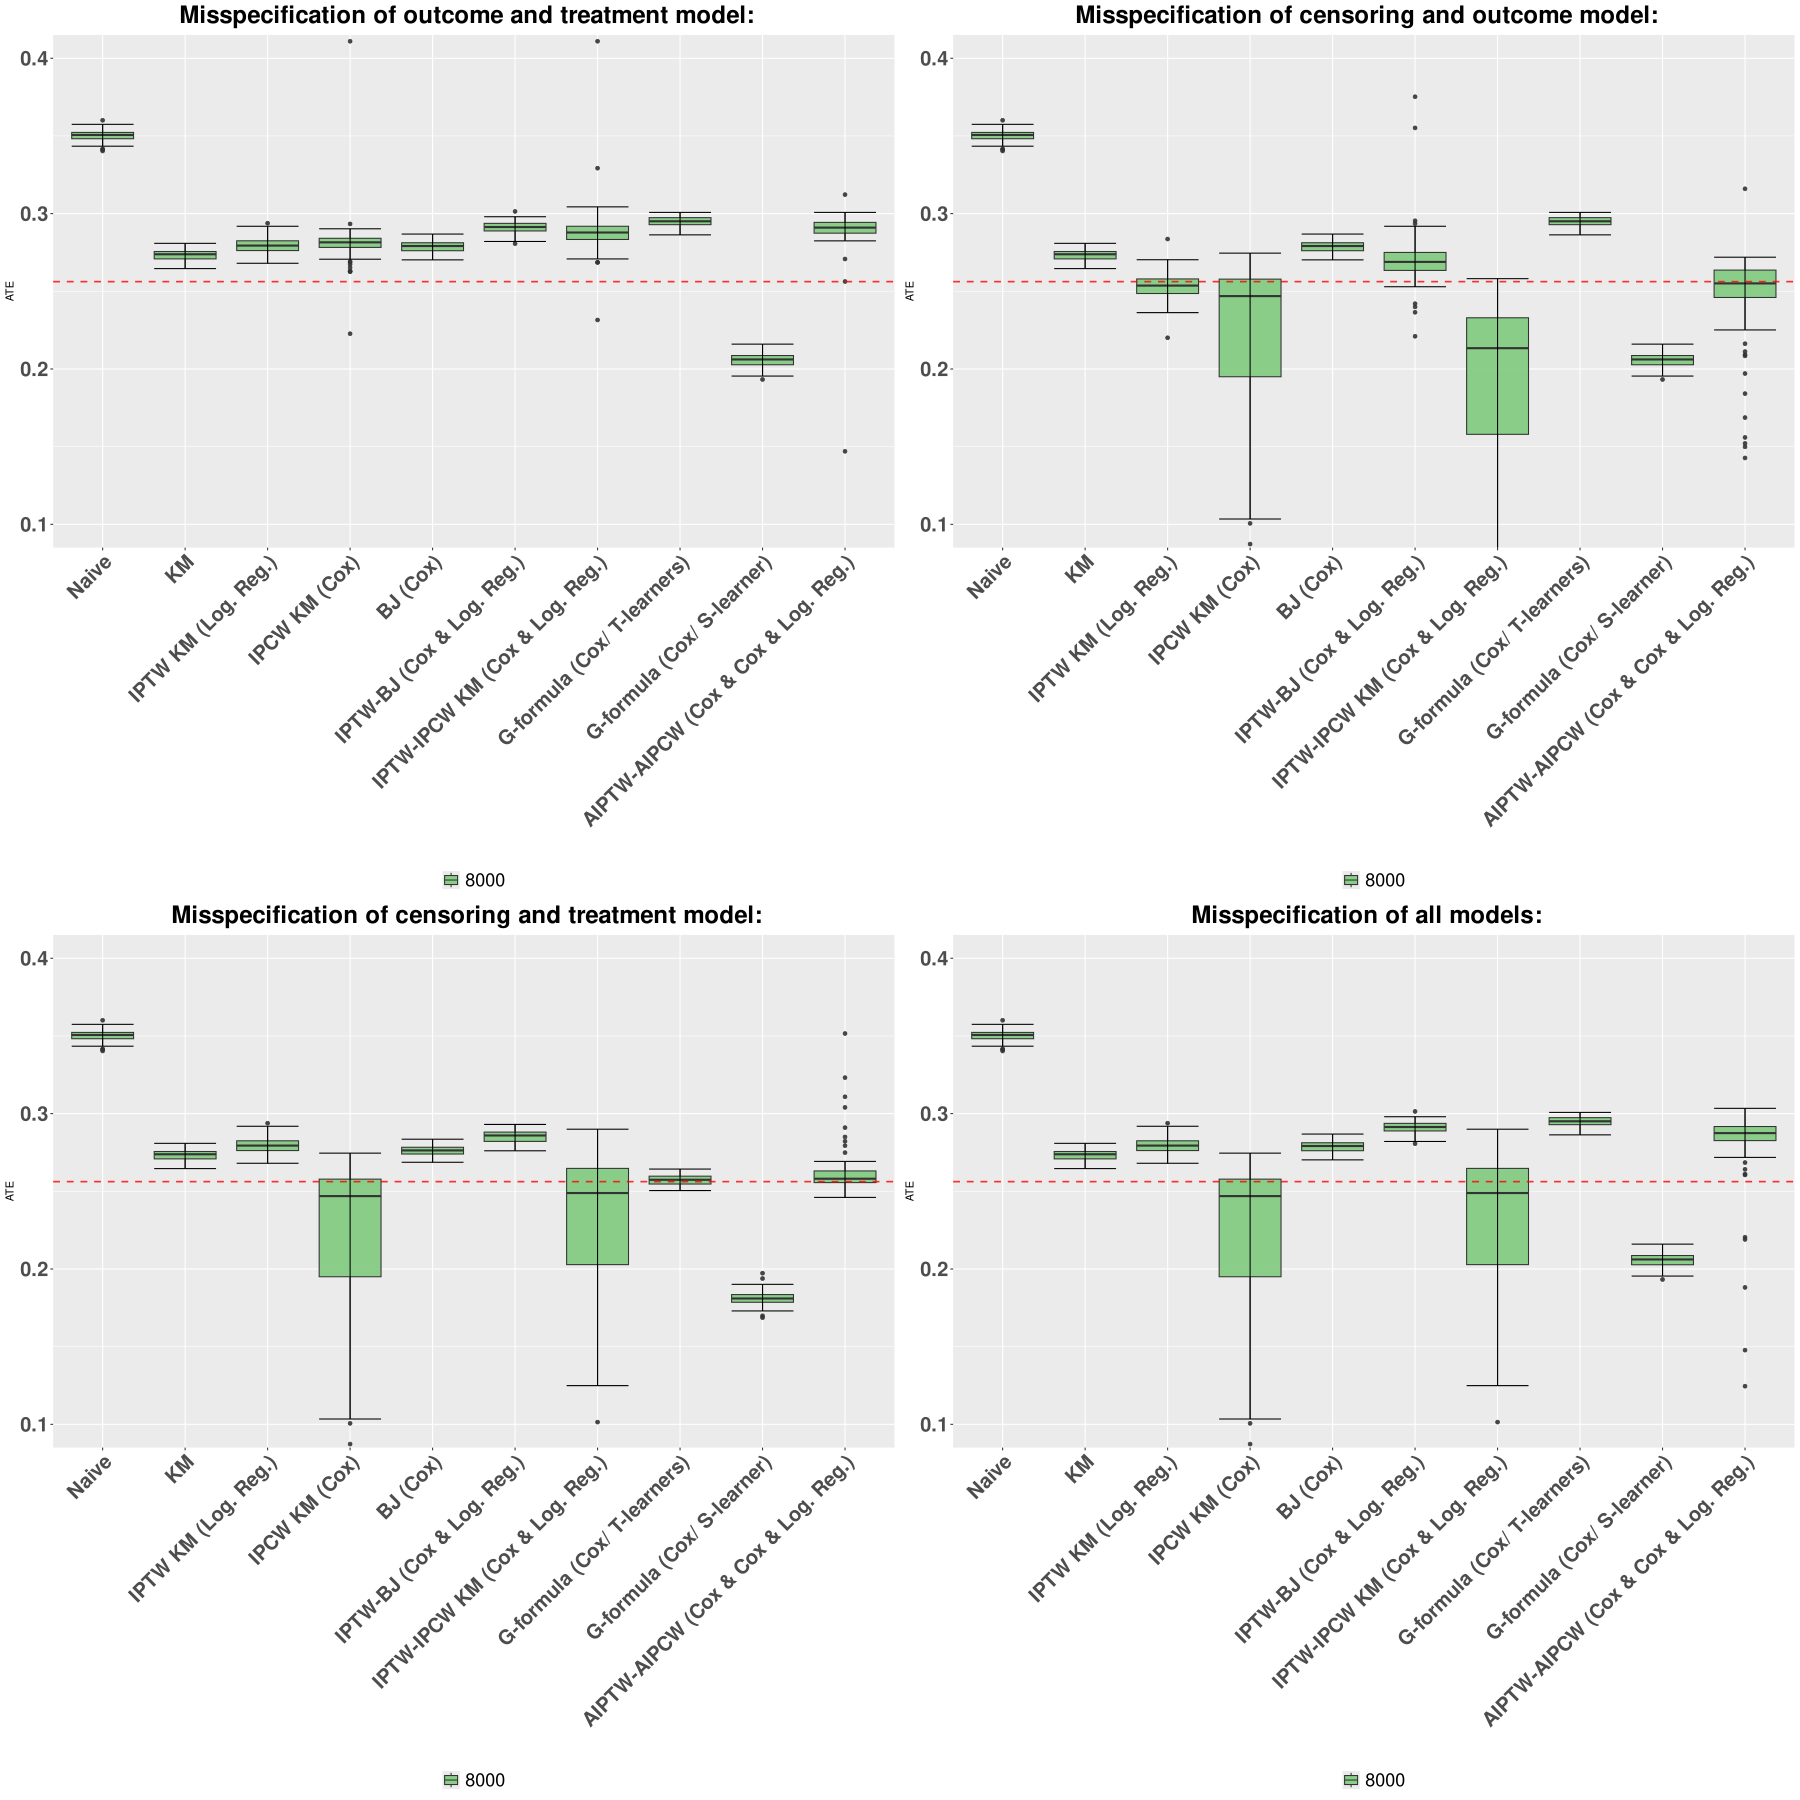
\includegraphics{Notebook_causal_survival_files/figure-pdf/fig-mis2-1.pdf}

}

\caption{\label{fig-mis2}Estimation results of the ATE for an
observational study with dependent censoring in case of a two or more
misspecifications.}

\end{figure}%

Figure~\ref{fig-mis2} shows that, as expected, when all nuisance models
are misspecified, all estimators exhibit bias. AIPTW-AIPCW (Cox \& Cox
\& Reg.Log) seems to converge in case where either the outcome and
censoring models, or the treatment and censoring models are
misspecificed which deviates from initial expectations. It was
anticipated that AIPTW-AIPCW would converge solely when both the
censoring and treatment models were misspecified.

\section{Conclusion}\label{sec-conclusion}

Based on the simulations and theoretical results, it might be advisable
to stay away from the IPCW and IPTW-IPCW estimators, as they often
exhibit excessive variability. Instead, we recommend implementing BJ
which seems like a more stable transformation as IPCW, as well as Causal
Survival Forest, G-formula (T-learners), IPTW-BJ, and AIPTW-AIPCW in
both their Cox, Logistic Regression and forest versions. By
qualitatively combining the results from these more robust estimators,
we can expect to gain a fairly accurate understanding of the treatment
effect.

It is important to note that our simulations utilize large sample sizes
with relatively simple relationships, which may not fully capture the
complexity of real-world scenarios. In practice, most survival analysis
datasets tend to be smaller and more intricate, meaning the stability of
certain estimators observed in our simulations may not generalize to
real-world applications. Testing these methods on real-world datasets
would provide a more comprehensive evaluation of their performance in
practical settings.

An interesting direction for future work would be to focus on variable
selection. Indeed, there is no reason to assume that the variables
related to censoring should be the same as those linked to survival or
treatment allocation. We could explore differentiating these sets of
variables and study the impact on the estimators' variance. Similarly to
causal inference settings without survival data, we might expect, for
instance, that adding precision variables----those solely related to the
outcome----could reduce the variance of the estimators.

Additionally, the estimators of the Restricted Mean Survival Time (RMST)
provide a valuable alternative to the Hazard Ratio. The analysis and
code provided with this article enables further exploration of the
advantages of the estimators of RMST for causal analysis in survival
studies. This could lead to a deeper understanding of how these
estimators can offer more stable and interpretable estimates of
treatment effects, particularly in complex real-world datasets.

\section*{References}\label{references}
\addcontentsline{toc}{section}{References}

\phantomsection\label{refs}
\begin{CSLReferences}{1}{0}
\bibitem[\citeproctext]{ref-Aalen2008}
Aalen, O., O. Borgan, and H. Gjessing. 2008. \emph{Survival and Event
History Analysis: A Process Point of View}. Statistics for Biology and
Health. Springer New York.
\url{https://books.google.de/books?id=wEi26X-VuCIC}.

\bibitem[\citeproctext]{ref-Breslow_approx1974}
Breslow, N. 1974. {``Covariance Analysis of Censored Survival Data.''}
\emph{Biometrics} 30 (1): 89--99.
\url{http://www.jstor.org/stable/2529620}.

\bibitem[\citeproctext]{ref-Kaplan_consistency_breslow74}
Breslow, N., and J. Crowley. 1974. {``{A Large Sample Study of the Life
Table and Product Limit Estimates Under Random Censorship}.''} \emph{The
Annals of Statistics} 2 (3): 437--53.
\url{https://doi.org/10.1214/aos/1176342705}.

\bibitem[\citeproctext]{ref-Buckley_james_79}
Buckley, and James. 1979. {``{Linear regression with censored data}.''}
\emph{Biometrika} 66 (3): 429--36.
\url{https://doi.org/10.1093/biomet/66.3.429}.

\bibitem[\citeproctext]{ref-RMST}
Chen, Pei-Yun, and Anastasios A. Tsiatis. 2001. {``Causal Inference on
the Difference of the Restricted Mean Lifetime Between Two Groups.''}
\emph{Biometrics} 57 (4): 1030--38.
\url{https://doi.org/10.1111/j.0006-341X.2001.01030.x}.

\bibitem[\citeproctext]{ref-colnet2022reweighting}
Colnet, Bénédicte, Julie Josse, Gaël Varoquaux, and Erwan Scornet. 2022.
{``Reweighting the RCT for Generalization: Finite Sample Error and
Variable Selection.''} \emph{arXiv Preprint arXiv:2208.07614}.

\bibitem[\citeproctext]{ref-Cox_1972}
Cox, D. R. 1972. {``Regression Models and Life-Tables.''} \emph{Journal
of the Royal Statistical Society: Series B (Methodological)} 34 (2):
187--202. \url{https://doi.org/10.1111/j.2517-6161.1972.tb00899.x}.

\bibitem[\citeproctext]{ref-HTE_causal_survival_forests}
Cui, Yifan, Michael R Kosorok, Erik Sverdrup, Stefan Wager, and Ruoqing
Zhu. 2023. {``{Estimating heterogeneous treatment effects with
right-censored data via causal survival forests}.''} \emph{Journal of
the Royal Statistical Society Series B: Statistical Methodology} 85 (2):
179--211. \url{https://doi.org/10.1093/jrsssb/qkac001}.

\bibitem[\citeproctext]{ref-ebrahimi2003identifiability}
Ebrahimi, Nader, Daniel Molefe, and Zhiliang Ying. 2003.
{``Identifiability and Censored Data.''} \emph{Biometrika} 90 (3):
724--27.

\bibitem[\citeproctext]{ref-EMA_RWD}
European Medecines Agency, EMA. 2024. {``Reflection Paper on Use of
Real-World Data in Non-Interventional Studies to Generate Real-World
Evidence.''}
\url{https://www.ema.europa.eu/en/reflection-paper-use-real-world-data-non-interventional-studies-generate-real-world-evidence-scientific-guideline}.

\bibitem[\citeproctext]{ref-fan2010high}
Fan, Jianqing, Yang Feng, and Yichao Wu. 2010. {``High-Dimensional
Variable Selection for Cox's Proportional Hazards Model.''} In
\emph{Borrowing Strength: Theory Powering Applications--a Festschrift
for Lawrence d. Brown}, 6:70--87. Institute of Mathematical Statistics.

\bibitem[\citeproctext]{ref-LocalLinear_Fan94}
Fan, Jianqing, and Irène Gijbels. 1994. {``Censored Regression: Local
Linear Approximations and Their Applications.''} \emph{Journal of the
American Statistical Association} 89 (426): 560--70.
\url{https://doi.org/10.1080/01621459.1994.10476781}.

\bibitem[\citeproctext]{ref-Foster_2011}
Foster, Jared C., Jeremy M. G. Taylor, and Stephen J. Ruberg. 2011.
{``Subgroup Identification from Randomized Clinical Trial Data.''}
\emph{Statistics in Medicine} 30 (24): 2867--80.
\url{https://doi.org/10.1002/sim.4322}.

\bibitem[\citeproctext]{ref-Foucher_Le_Borgne_Chatton_2019}
Foucher, Yohann, Florent Le Borgne, and Arthur Chatton. 2019. {``RISCA:
Causal Inference and Prediction in Cohort-Based Analyses.''} \emph{CRAN:
Contributed Packages}. The R Foundation.
\url{https://doi.org/10.32614/cran.package.risca}.

\bibitem[\citeproctext]{ref-gill1983large}
Gill, Richard. 1983. {``Large Sample Behaviour of the Product-Limit
Estimator on the Whole Line.''} \emph{The Annals of Statistics}, 49--58.

\bibitem[\citeproctext]{ref-SurvRM2_2015}
Hajime, Uno, Tian Lu, Horiguchi Miki, Cronin Angel, Battioui Chakib, and
Bell James. 2015. {``survRM2: Comparing Restricted Mean Survival
Time.''} \emph{CRAN: Contributed Packages}. The R Foundation.
\url{https://doi.org/10.32614/cran.package.survrm2}.

\bibitem[\citeproctext]{ref-hernan2010causal}
Hernán, Miguel A, and James M Robins. 2010. {``Causal Inference.''} CRC
Boca Raton, FL.

\bibitem[\citeproctext]{ref-hirano2003efficient}
Hirano, Keisuke, Guido W Imbens, and Geert Ridder. 2003. {``Efficient
Estimation of Average Treatment Effects Using the Estimated Propensity
Score.''} \emph{Econometrica} 71 (4): 1161--89.

\bibitem[\citeproctext]{ref-Howe2016SelectionBD}
Howe, Chanelle J, Stephen R. Cole, Bryan Lau, Sonia Napravnik, and
Joseph J. Eron. 2016. {``Selection Bias Due to Loss to Follow up in
Cohort Studies.''} \emph{Epidemiology} 27 1: 91--97.
\url{https://api.semanticscholar.org/CorpusID:21993915}.

\bibitem[\citeproctext]{ref-huitfeldt2019collapsibility}
Huitfeldt, A., M. Stensrud, and E. Suzuki. 2019. {``On the
Collapsibility of Measures of Effect in the Counterfactual Causal
Framework.''} \emph{Emerging Themes in Epidemiology} 16: 1--12.

\bibitem[\citeproctext]{ref-ishwaran2008random}
Ishwaran, Hemant, Udaya B. Kogalur, Eugene H. Blackstone, and Michael S.
Lauer. 2008. {``{Random survival forests}.''} \emph{The Annals of
Applied Statistics} 2 (3): 841--60.
\url{https://doi.org/10.1214/08-AOAS169}.

\bibitem[\citeproctext]{ref-kalbfleisch2002statistical}
Kalbfleisch, John D, and Ross L Prentice. 2002. \emph{The Statistical
Analysis of Failure Time Data}. John Wiley \& Sons.

\bibitem[\citeproctext]{ref-kaplan}
Kaplan, E. L., and Paul Meier. 1958. {``Nonparametric Estimation from
Incomplete Observations.''} \emph{Journal of the American Statistical
Association} 53 (282): 457--81.
\url{https://doi.org/10.1080/01621459.1958.10501452}.

\bibitem[\citeproctext]{ref-IPCtransKoul81}
Koul, H., V. Susarla, and J. Van Ryzin. 1981. {``{Regression Analysis
with Randomly Right-Censored Data}.''} \emph{The Annals of Statistics} 9
(6): 1276--88. \url{https://doi.org/10.1214/aos/1176345644}.

\bibitem[\citeproctext]{ref-Soren_2019}
Künzel, Sören R., Jasjeet S. Sekhon, Peter J. Bickel, and Bin Yu. 2019.
{``Metalearners for Estimating Heterogeneous Treatment Effects Using
Machine Learning.''} \emph{Proceedings of the National Academy of
Sciences} 116 (10): 4156--65.
\url{https://doi.org/10.1073/pnas.1804597116}.

\bibitem[\citeproctext]{ref-vanderLaan2003}
Laan, Mark J. van der, and James M. Robins. 2003. {``Introduction.''} In
\emph{Unified Methods for Censored Longitudinal Data and Causality},
8--101. New York, NY: Springer New York.
\url{https://doi.org/10.1007/978-0-387-21700-0_1}.

\bibitem[\citeproctext]{ref-HR_Martinussen}
Martinussen, Torben, Stijn Vansteelandt, and Per Andersen. 2020.
{``Subtleties in the Interpretation of Hazard Contrasts.''}
\emph{Lifetime Data Analysis} 26 (October).
\url{https://doi.org/10.1007/s10985-020-09501-5}.

\bibitem[\citeproctext]{ref-Ozenne20_AIPTW_AIPCW}
Ozenne, Brice Maxime Hugues, Thomas Harder Scheike, Laila Stærk, and
Thomas Alexander Gerds. 2020. {``On the Estimation of Average Treatment
Effects with Right-Censored Time to Event Outcome and Competing
Risks.''} \emph{Biometrical Journal} 62 (3): 751--63.
\url{https://doi.org/10.1002/bimj.201800298}.

\bibitem[\citeproctext]{ref-robins1994estimation}
Robins, James M., Andrea Rotnitzky, and Lue Ping Zhao. 1994.
{``Estimation of Regression Coefficients When Some Regressors Are Not
Always Observed.''} \emph{Journal of the American Statistical
Association} 89 (427): 846--66.

\bibitem[\citeproctext]{ref-Propensity_causality}
Rosenbaum, Paul R., and Donald B. Rubin. 1983. {``{The central role of
the propensity score in observational studies for causal effects}.''}
\emph{Biometrika} 70 (1): 41--55.
\url{https://doi.org/10.1093/biomet/70.1.41}.

\bibitem[\citeproctext]{ref-royston2013restricted}
Royston, Patrick, and Mahesh KB Parmar. 2013. {``Restricted Mean
Survival Time: An Alternative to the Hazard Ratio for the Design and
Analysis of Randomized Trials with a Time-to-Event Outcome.''} \emph{BMC
Medical Research Methodology} 13: 1--15.

\bibitem[\citeproctext]{ref-DoublyR_transformation}
Rubin, Daniel, and Mark J. van der Laan. 2007. \emph{The International
Journal of Biostatistics} 3 (1).
\url{https://doi.org/10.2202/1557-4679.1052}.

\bibitem[\citeproctext]{ref-rubin_estimating_1974}
Rubin, Donald B. 1974. {``Estimating Causal Effects of Treatments in
Randomized and Nonrandomized Studies.''} \emph{Journal of Educational
Psychology} 66 (5): 688--701. \url{https://doi.org/10.1037/h0037350}.

\bibitem[\citeproctext]{ref-Schaubel2011}
Schaubel, Douglas E., and Guanghui Wei. 2011. {``{Double
Inverse-Weighted Estimation of Cumulative Treatment Effects under
Nonproportional Hazards and Dependent Censoring}.''} \emph{Biometrics}
67 (1): 29--38. \url{https://doi.org/10.1111/j.1541-0420.2010.01449.x}.

\bibitem[\citeproctext]{ref-Therneau_2001}
Therneau, Terry M. 2001. {``Survival: Survival Analysis.''} \emph{CRAN:
Contributed Packages}. The R Foundation.
\url{https://doi.org/10.32614/cran.package.survival}.

\bibitem[\citeproctext]{ref-Tibshirani_Athey_Sverdrup_Wager_2017}
Tibshirani, Julie, Susan Athey, Erik Sverdrup, and Stefan Wager. 2017.
{``Grf: Generalized Random Forests.''} \emph{CRAN: Contributed
Packages}. The R Foundation.
\url{https://doi.org/10.32614/cran.package.grf}.

\bibitem[\citeproctext]{ref-censoring_effect}
Turkson, Anthony, Francis Ayiah-Mensah, and Vivian Nimoh. 2021.
{``Handling Censoring and Censored Data in Survival Analysis: A
Standalone Systematic Literature Review.''} \emph{International Journal
of Mathematics and Mathematical Sciences} 2021 (September): 1--16.
\url{https://doi.org/10.1155/2021/9307475}.

\bibitem[\citeproctext]{ref-IPTW}
Xie, Jun, and Chaofeng Liu. 2005. {``Adjusted Kaplan--Meier Estimator
and Log-Rank Test with Inverse Probability of Treatment Weighting for
Survival Data.''} \emph{Statistics in Medicine} 24 (20): 3089--3110.
\url{https://doi.org/10.1002/sim.2174}.

\bibitem[\citeproctext]{ref-zhang2016parametric}
Zhang, Zhongheng. 2016. {``Parametric Regression Model for Survival
Data: Weibull Regression Model as an Example.''} \emph{Annals of
Translational Medicine} 4 (24).

\bibitem[\citeproctext]{ref-zhou1988two}
Zhou, M. 1988. {``Two-Sided Bias Bound of the Kaplan-Meier Estimator.''}
\emph{Probability Theory and Related Fields} 79 (2): 165--73.

\end{CSLReferences}

\section{Appendix A: Proofs}\label{appendix-a-proofs}

\subsection{\texorpdfstring{Proofs of
Section~\ref{sec-theoryRCT_indc}}{Proofs of Section~}}\label{sec-proof21}

\begin{proof}
\emph{(Proposition~\ref{prp-km}).} Consistency is a trivial consequence
of the law of large number and the identity \ref{eq-kmi}. To show that
\(\widehat S_{\mathrm{KM}}\) is unbiased, let us introduce
\(\mathcal{F}_k\) be the filtration generated by the set of variables \[
\{A_i, \mathbb{I}\{\widetilde T_i = t_j\}, \mathbb{I}\{\widetilde T_i = t_j, \Delta_i=1\}~|~j \in [k], i \in [n]\}.
\] which corresponds to the known information up to time \(t_k\), so
that \(D_k(a)\) is \(\mathcal{F}_k\)-measurable but \(N_k(a)\) is
\(\mathcal{F}_{k-1}\)-measurable. One can write that, for
\(k\geqslant 2\) \begin{align*}
\mathbb{E}[\mathbb{I}\{\widetilde T_i = t_k, \Delta_i = 1, A_i=a\}~|~\mathcal{F}_{k-1}] &= \mathbb{E}[\mathbb{I}\{\widetilde T_i = t_k, \Delta_i = 1, A_i=a\}~|~\mathbb{I}\{\widetilde T_i \geqslant t_k\},A_i]  \\
&= \mathbb{I}\{A_i=a\} \mathbb{E}[\mathbb{I}\{T_i = t_k, C_i \geqslant t_k\}~|~\mathbb{I}\{T_i \geqslant t_k, C_i \geqslant t_k\}, A_i] \\
&=  \mathbb{I}\{A_i=a\} \mathbb{I}\{C_i \geqslant t_k\} \mathbb{E}[\mathbb{I}\{T_i = t_k\} ~|~ \mathbb{I}\{T_i \geqslant t_k\}, A_i] \\
&= \mathbb{I}\{\widetilde T_i \geqslant t_k, A_i=a\}\left(1- \frac{S^{(a)}(t_{k})}{S^{(a)}(t_{k-1})}\right),
\end{align*} where we used that \(T_i(a)\) is idependant from \(A_i\) by
Assumption \ref{eq-rta}. We then easily derive from this that \[
\mathbb{E}\left[\left(1-\frac{D_k(a)}{N_k(a)} \right) \mathbb{I}\{N_k(a) >0\}\middle |\mathcal{F}_{k-1}\right] = \frac{S^{(a)}(t_k)}{S^{(a)}(t_{k-1})} \mathbb{I}\{N_k(a) >0\},
\] and then that \[
\mathbb{E}\left[\widehat S_{\mathrm{KM}}(t_k|A=a)\middle |\mathcal{F}_{k-1}\right] =  \frac{S^{(a)}(t_k)}{S^{(a)}(t_{k-1})} \widehat S_{\mathrm{KM}}(t_{k-1}|A=a) + O(\mathbb{I}\{N_k(a) =0\}),
\]

By induction, we easily find that \[
\mathbb{E}[\widehat S_{\mathrm{KM}}(t|A=a)] = \prod_{t_j \leqslant t} \frac{S^{(a)}(t_j)}{S^{(a)}(t_{j-1})} + O\left(\sum_{t_j \leqslant t}\mathbb{P}(N_j(a) =0)\right)= S^{(a)}(t) + O(\mathbb{P}(N_k(a) =0))
\] where \(t_k\) is the greatest time such that \(t_k \leqslant t\).
\end{proof}

\begin{proof}
\emph{(Proposition~\ref{prp-varkm}).} The asymptotic normality is a mere
consequence of the joint asymptotic normality of
\((N_k(a),D_k(a))_{t_k \leqslant t}\) with an application of the
\(\delta\)-method. To access the asymptotic variance, notice that, using
a similar reasonning as in the previous proof: \begin{align*}
\mathbb{E}[(1-D_k(a)/N_k(a))^2|\mathcal{F}_{k-1}] &= \mathbb{E}[1-D_k(a)/N_k(a)|\mathcal{F}_{k-1}(a)]^2+\frac{1}{N_k(a)^2}\mathrm{Var}(D_k(a)|\mathcal{F}_{k-1}) \\
&= s_k^2(a)+ \frac{s_k(a)(1-s_k(a))}{N_k(a)}\mathbb{I}\{N_k(a) > 0\} + O(\mathbb{I}\{N_k(a) = 0\}). 
\end{align*} Now we know that
\(N_k(a) = n r_k(a) + \sqrt{n} O_{\mathbb{P}}(1)\), with the
\(O_{\mathbb{P}}(1)\) having uniformly bounded moments. So that we
deduce that \[
\begin{aligned}
\mathbb{E}[(1-D_k(a)/N_k(a))^2|\mathcal{F}_{k-1}] &= s_k^2(a)+ \frac{s_k(a)(1-s_k(a))}{n r_k(a)} +  \frac{1}{n^{3/2}} O_{\mathbb{P}}(1), 
\end{aligned}
\] where \(O_{\mathbb{P}}(1)\) has again bounded moments. Using this
identity, we find that \[
\begin{aligned}
n \mathrm{Var}\widehat S_{\mathrm{KM}} (t|A=a) &= n \left(\mathbb{E}S_{\mathrm{KM}} (t|A=a)^2 -  S^{(a)} (t)^2 \right) \\
&= n S^{(a)}(t)^2 \left(\mathbb{E}\left[\prod_{t_k \leqslant t}  \left(1+\frac1n\frac{1-s_k(a)}{s_k(a) r_k(a)} +   \frac{1}{n^{3/2}} O_{\mathbb{P}}(1) \right)\right]-1\right).
\end{aligned}
\] Expending the product and using that the \(O_{\mathbb{P}}(1)\)'s have
bounded moments, we finally deduce that \[
\begin{aligned}
\mathbb{E}\left[\prod_{t_k \leqslant t}  \left(1+\frac1n\frac{1-s_k(a)}{s_k(a) r_k(a)} +   \frac{1}{n^{3/2}} O_{\mathbb{P}}(1) \right)\right]-1 =   \frac1n \sum_{t_k \leqslant t}\frac{1-s_k(a)}{s_k(a) r_k(a)} +   \frac{1}{n^{3/2}} O(1),
\end{aligned}
\]

\[
n\mathrm{Var}\widehat S_{\mathrm{KM}} (t|A=a) = V_{\mathrm{KM}}(t|A=a) + O(n^{-1/2}),  
\] which is what we wanted to show.
\end{proof}

\subsection{\texorpdfstring{Proofs of
Section~\ref{sec-condcens}}{Proofs of Section~}}\label{sec-proof22}

\begin{proof}
\emph{(Proposition~\ref{prp-ipcw}).} Assumption
\ref{eq-positivitycensoring} allows the tranformation to be
well-defined. Furthermore, it holds \begin{align*}
E[T^*_{\mathrm{IPCW}}|A=a,X] 
&= E\left[\frac{ \Delta^\tau \times\widetilde T \wedge \tau}{G(\widetilde T \wedge \tau | A,X)} \middle | A = a,X\right]  \\
&= E\left[\frac{ \Delta^\tau \times T(a) \wedge \tau}{G(T(a) \wedge \tau | A,X)} \middle | A = a,X\right]\\
&= E\left[ E\left[\frac{ \mathbb{I}\{T(a)\wedge \tau \leqslant C \} \times T(a) \wedge \tau}{G(T(a) \wedge \tau | A,X)}\middle| A, X,T(1) \right] \middle | A = a,X\right] \\
&= E\left[T(a) \wedge \tau|A=a, X\right] \\
&= E\left[T(a) \wedge \tau | X \right].
\end{align*} We used in the second equality that on the event
\(\{\Delta^\tau=1, A=a\}\), it holds
\(\widetilde T \wedge \tau =  T \wedge \tau = T(a) \wedge \tau\). We
used in the fourth equality that
\(G(T(a) \wedge \tau | A,X) = E[\mathbb{I}\{T(a) \wedge \tau \leqslant C\}|X,T(a),A]\)
thanks to Assumption \ref{eq-condindepcensoring}, and in the last one
that \(A\) is idependent from \(X\) and \(T(a)\) thanks to Assumption
\ref{eq-rta}.
\end{proof}

\begin{proof}
\emph{(Proposition~\ref{prp-ipcwkm}).} Similarly to the computations
done in the proof of Proposition~\ref{prp-ipcw}, it is easy to show that
\[
\mathbb{E}\left[\frac{\Delta_i^\tau}{G(\widetilde T \wedge\tau | X,A)} \mathbb{I}(\widetilde T_i = t_k, A=a)\right] = \mathbb{P}(A=a) \mathbb{P}(T(a) = t_k),
\] and likewise that \[
\mathbb{E}\left[\frac{\Delta_i^\tau}{G(\widetilde T \wedge\tau | X,A)} \mathbb{I}(\widetilde T_i \geqslant t_k, A=a)\right] = \mathbb{P}(A=a) \mathbb{P}(T(a) \geqslant t_k),
\] so that \(\widehat S_{\mathrm{IPCW}}(t)\) converges almost surely
towards the product limit \[
\prod_{t_k \leqslant t} \left(1-\frac{\mathbb{P}(T(a) = t_k)}{\mathbb{P}(T(a) \geqslant t_k)}\right) = S^{(a)}(t),
\] yielding strong consistency. Asymptotic normality is straightforward.
\end{proof}

\begin{proof}
\emph{(Proposition~\ref{prp-bj}).} There holds \[
\begin{aligned}
\mathbb{E}[T_{\mathrm{BJ}}^*|X,A=a] &= \mathbb{E}\left[\Delta^\tau T(a) \wedge \tau + (1-\Delta^\tau)\frac{\mathbb{E}[T \wedge \tau \times \mathbb{I}\{T \wedge \tau > C\}|C,A,X]}{\mathbb{P}(T > C|C,A,X)} \middle | X,A=a \right] \\
&= \mathbb{E}[\Delta^\tau T(a) \wedge \tau | X ] +  \underbrace{\mathbb{E}\left[ \mathbb{I}\{T \wedge \tau > C\} \frac{\mathbb{E}[T \wedge \tau \times \mathbb{I}\{T \wedge \tau > C\}|C,A,X]}{\mathbb{E}[\mathbb{I}\{T \wedge \tau \geqslant C\}|C,A,X]}\middle | X,A=a \right]}_{(\star)}.
\end{aligned}
\] Now we easily see that conditionning wrt \(X\) in the second term
yields \begin{align*}
(\star) &= \mathbb{E}\left[ \mathbb{E}[T \wedge \tau \times \mathbb{I}\{T \wedge \tau > C\}|C,A,X] \middle | X,A=a \right] \\
&= \mathbb{E}[(1-\Delta^\tau) T \wedge \tau | X,A=a ]  \\
&= \mathbb{E}[(1-\Delta^\tau)  T(a) \wedge \tau | X], 
\end{align*} ending the proof.
\end{proof}

\begin{proof}
\emph{(Theorem~\ref{thm-bj}).} We let
\(T^* = \Delta^\tau \phi_1 + (1-\Delta^\tau)\phi_0\) be a transformation
of the form Equation~\ref{eq-defcut}. There holds \[
\mathbb{E}[(T^*-T \wedge \tau)^2] = \mathbb{E}[\Delta^\tau (\phi_1-T \wedge \tau)^2] + \mathbb{E}[(1-\Delta^\tau)(\phi_0-T \wedge \tau)^2].
\] The first term is non negative and is zero for the BJ transformation.
Since \(\phi_0\) is a function of \((\widetilde T, X, A)\) and that
\(\widetilde T = C\) on \(\{\Delta^\tau = 0\}\), the second term can be
rewritten in the following way. We let \(R\) be a generic quantity that
does not depend on \(\phi_0\). \begin{align*}
\mathbb{E}&[(1-\Delta^\tau)(\phi_0-T)^2] = \mathbb{E}\left[\mathbb{I}\{T\wedge \tau > C\} \phi_0^2 - 2 \mathbb{I}\{T\wedge \tau > C\} \phi_0 T \wedge \tau\right]  + R \\
&= \mathbb{E}\left[ \mathbb{P}(T\wedge \tau > C|C,A,X) \phi_0^2 - 2 \mathbb{E}[T\wedge \tau \mathbb{I}\{T\wedge \tau > C\}|C,A,X] \phi_0 \right] + R \\
&= \mathbb{E}\left[\mathbb{P}(T\wedge \tau > C|C,A,X) \left(\phi_0- \frac{\mathbb{E}[T\wedge \tau \mathbb{I}\{T\wedge \tau > C\}|C,A,X]}{\mathbb{P}(T\wedge \tau > C|C,A,X) }\right)^2\right] + R.
\end{align*} Now the first term in the right hand side is always
non-negative, and is zero for the BJ tranformation.
\end{proof}

\subsection{\texorpdfstring{Proofs of
Section~\ref{sec-obs_indcen}}{Proofs of Section~}}\label{sec-proof31}

\begin{proof}
\emph{(Proposition~\ref{prp-iptwkm}).} The fact that it is strongly
consistent and asymptotically normal is again a simple application of
the law of large number and of the \(\delta\)-method. We indeed find
that, for \(t_k \leqslant\tau\) \[
\begin{aligned}
\mathbb{E}\left[\frac{1}{e(X_i)} \mathbb{1}\{\widetilde T_i = t_k, \Delta_i = 1, A_i=1\}\right] &= \mathbb{E}\left[\frac{A_i}{e(X_i)} \mathbb{1}\{T_i = t_k, C_i \geqslant t_k\}\right] \\
&=\mathbb{E}\left[ \mathbb{E}\left[ \frac{A_i}{e(X_i)} \mathbb{1}\{T_i = t_k, C_i \geqslant t_k\} \middle |X_i \right]\right] \\
&= \mathbb{E}\left[ \mathbb{E}\left[\frac{A_i}{e(X_i)}\middle | X_i\right] \mathbb{P}(T_i = t_k |X_i) \mathbb{P}( C_i \geqslant t_k)\right] \\
&= \mathbb{P}(T_i = t_k) \mathbb{P}( C_i \geqslant t_k),
\end{aligned}
\] where we used that \(A\) is independent from \(T\) conditionnaly on
\(X\), and that \(C\) is independent from everything. Likewise, one
would get that \[
\begin{aligned}
\mathbb{E}\left[\frac{1}{e(X_i)} \mathbb{1}\{\widetilde T_i \geqslant t_k, A_i=1\}\right] =
&= \mathbb{P}(T_i \geqslant t_k) \mathbb{P}( C_i \geqslant t_k).
\end{aligned}
\] Similar computations hold for \(A=0\), ending the proof.
\end{proof}

\subsection{\texorpdfstring{Proofs of
Section~\ref{sec-obscondcens}}{Proofs of Section~}}\label{sec-proof32}

\begin{proof}
\emph{(Proposition~\ref{prp-iptwipcw}).} On the event
\(\{\Delta^\tau=1, A=1\}\), there holds
\(\widetilde T \wedge \tau = T \wedge \tau = T(1) \wedge \tau\), whence
we find that, \[
\begin{aligned}
\mathbb{E}[ T^*_{\mathrm{IPCW}}|X,A=1] &= \mathbb{E}\left[\frac{A}{e(X)} \frac{\mathbb{I}\{T(1) \wedge \tau \leqslant C\}}{G(T(1) \wedge \tau|X,A)} T(1) \wedge \tau\middle|X\right] \\
&= \mathbb{E}\left[ \frac{A}{e(X)} \mathbb{E}\left[\frac{\mathbb{I}\{T(1) \wedge \tau \leqslant C\}}{G(T(1) \wedge \tau|X,A)} \middle| X,A, T(1) \right]T(1) \wedge \tau\middle|X\right] \\
&=\mathbb{E}\left[ \frac{A}{e(X)} T(1) \wedge \tau\middle|X\right] \\
&=\mathbb{E}\left[T(1) \wedge \tau\middle|X\right],
\end{aligned}
\] and the same holds on the event \(A=0\).
\end{proof}

\begin{proof}
\emph{(Proposition~\ref{prp-consiptwipcw}).} By consistency of
\(\widehat G(\cdot|X,A)\) and \(\widehat e\) and by continuity, it
suffices to look at the asymptotic behavior of the oracle estimator \[
\theta^*_{\mathrm{IPTW-IPCW}} = \frac1n\sum_{i=1}^n  \left(\frac{A_i}{ e(X_i)}-\frac{1-A_i}{1-e(X_i)} \right)\frac{\Delta_i^\tau}{G(\widetilde T_i \wedge \tau | A_i,X_i)} \widetilde T_i \wedge \tau.
\] The later is converging almost towards its mean, which, following
similar computations as in the previous proof, write \[
\begin{aligned}
\mathbb{E}\left[\left(\frac{A}{e(X)}-\frac{1-A}{1-e(X)} \right)\frac{\Delta^\tau}{G(\widetilde T \wedge \tau | A,X)} \widetilde T \wedge \tau\right]  
&= \mathbb{E}\left[\left(\frac{A}{e(X)}-\frac{1-A}{1-e(X)} \right) T \wedge \tau\right] \\
&= \mathbb{E}\left[T(1) \wedge \tau\right]-\mathbb{E}\left[T(0) \wedge \tau\right].
\end{aligned}
\]
\end{proof}

\begin{proof}
\emph{(Proposition~\ref{prp-iptwipcwkm}).} Asymptotic normality comes
from a mere application of the \(\delta\)-method, while strong
consistency follows from the law of large number and the follozing
computations. Like for the proof of Proposition~\ref{prp-ipcwkm}, one
find, by first conditionning wrt \(X,A,T(a)\), that, for
\(t_k \leqslant\tau\), \[
\begin{aligned}
\mathbb{E}\left[\left(\frac{A}{e(X)}+\frac{1-A}{1-e(X)} \right)\frac{\Delta^\tau}{G(\widetilde T \wedge \tau | A,X)} \mathbb{I}\{\widetilde T = t_k, A=a\}\right] = \mathbb{P}(T(a)=t_k)
\end{aligned}
\] and likewise that \[
\begin{aligned}
\mathbb{E}\left[\left(\frac{A}{e(X)}+\frac{1-A}{1-e(X)} \right)\frac{\Delta^\tau}{G(\widetilde T \wedge \tau | A,X)} \mathbb{I}\{\widetilde T \geqslant t_k, A=a\}\right] = \mathbb{P}(T(a)\geqslant t_k)
\end{aligned}
\] so that indeed \(S^*_{\mathrm{IPTW-IPCW}} (t|A=a)\) converges almost
surely towards \(S^{(a)}(t)\).
\end{proof}

\begin{proof}
\emph{(Proposition~\ref{prp-iptwbj}).} We write \[
\begin{aligned}
\mathbb{E}[ T^*_{\mathrm{IPTW-BJ}}|X,A=1] &= \mathbb{E}\left[\frac{A}{e(X)} \Delta^\tau \times \widetilde T \wedge \tau\middle|X\right] + \mathbb{E}\left[\frac{A}{e(X)} (1-\Delta^\tau) Q_S(\widetilde T \wedge \tau|A,X) \middle| X\right]. 
\end{aligned}
\] On the event \(\{\Delta^\tau=1, A=1\}\), there holds
\(\widetilde T \wedge \tau = T \wedge \tau = T(1) \wedge \tau\), whence
we find that the first term on the the right hand side is equal to \[
\begin{aligned}
\mathbb{E}\left[\frac{A}{e(X)} \Delta^\tau \times \widetilde T \wedge \tau\middle|X\right] &= \mathbb{E}\left[\frac{A}{e(X)} \Delta^\tau \times T(1) \wedge \tau\middle|X\right] \\
&= \mathbb{E}\left[\Delta^\tau \times T(1) \wedge \tau\middle|X\right].
\end{aligned}
\] For the second term in the right hand side, notice that on the event
\(\{\Delta^\tau=0, A=1\}\), there holds
\(\widetilde T = C < T(1) \wedge \tau\), so that \[
\begin{aligned}
\mathbb{E}&\left[\frac{A}{e(X)} \mathbb{I}\{C < T(1) \wedge \tau\} \frac{\mathbb{E}[T(1) \wedge \tau \times \mathbb{I}\{C < T(1) \wedge \tau\}|X,A,C]}{\mathbb{P}(C < T(1) \wedge \tau | C,X,A)} \middle| X\right] \\
&= \mathbb{E}\left[\frac{A}{e(X)} \mathbb{E}[T(1) \wedge \tau \times \mathbb{I}\{C < T(1) \wedge \tau\}|X,A,C] \middle| X\right] \\
&= \mathbb{E}\left[T(1) \wedge \tau \times \mathbb{I}\{C < T(1) \wedge \tau\} \middle| X\right] \\
&= \mathbb{E}\left[(1-\Delta^\tau) T(1) \wedge \tau  \middle| X\right], 
\end{aligned}
\] and the sane holds on the event \(\{A=0\}\), which ends the proof.
\end{proof}

\begin{proof}
\emph{(Proposition~\ref{prp-consiptwbj}).} By consistency of
\(\widehat G(\cdot|X,A)\) and \(\widehat e\) and by continuity, it
suffices to look at the asymptotic behavior of the oracle estimator \[
\theta^*_{\mathrm{IPTW-BJ}} = \frac1n\sum_{i=1}^n  \left(\frac{A_i}{ e(X_i)}-\frac{1-A_i}{1-e(X_i)} \right)\left(\Delta_i^\tau \times \widetilde T_i \wedge \tau + (1-\Delta_i^\tau) Q_S(\widetilde T_i \wedge \tau|A_i,X_i)\right).
\] The later is converging almost towards its mean, which, following
similar computations as in the previous proof, is simply equal to the
difference in RMST.
\end{proof}

\begin{proof}
\emph{(Proposition~\ref{prp-tqr}).} We can write that \[
\Delta^*_{\mathrm{QR}} = \underbrace{\frac{A}{p(X)}(T^*_{\mathrm{DR}}(F,R)-\nu(X,1))+ \nu(X,1)}_{(\mathrm{A})} - \left(\underbrace{\frac{1-A}{1-p(X)}(T^*_{\mathrm{DR}}(F,R)-\nu(X,0))+ \nu(X,0)}_{(\mathrm{B})} \right). 
\] Focusing on term \((\mathrm{A})\), we easily find that \[
\begin{aligned}
\mathbb{E}[(\mathrm{A}) |X] &= \mathbb{E}\left[\frac{A}{p(X)}(T^*_{\mathrm{DR}}(F,R)-\nu(X,1))+ \nu(X,1) \middle|X\right] \\
&= \frac{e(X)}{p(X)}(\mu(X,1)-\nu(X,1)) + \nu(X,1).
\end{aligned}
\] Where we used that \(T^*_{\mathrm{DR}}(F,R)\) is a censoring unbiased
transform when \(F=G\) or \(R=S\). Now we see that if \(p(X) = e(X)\),
then \[
\mathbb{E}[(\mathrm{A}) |X] = \mu(X,1)-\nu(X,1) + \nu(X,1) = \mu(X,1),
\] and if \(\nu(X,1) = \mu(X,1)\), then \[
\mathbb{E}[(\mathrm{A}) |X] = \frac{e(X)}{p(X)} \times 0 + \mu(X,1) = \mu(X,1).
\] Likewise, we would show that
\(\mathbb{E}[(\mathrm{B}) |X] = \mu(X,0)\) under either alternative,
ending the proof.
\end{proof}

\section{Appendix B: Descriptive
statistics}\label{appendix-b-descriptive-statistics}

\subsection{RCT}\label{sec-stat_RCT}

The summary by group of treatment of the generated (observed and
unobserved) RCT with independent censoring is displayed below:

\begin{verbatim}
[1] "Descriptive statistics for group A=0:   996"
\end{verbatim}

\begin{verbatim}
       X1                X2                X3                X4         
 Min.   :-2.3677   Min.   :-2.0217   Min.   :-4.2566   Min.   :-2.5973  
 1st Qu.: 0.3504   1st Qu.: 0.3189   1st Qu.:-1.6666   1st Qu.: 0.3297  
 Median : 1.0350   Median : 1.0020   Median :-1.0246   Median : 1.1204  
 Mean   : 0.9893   Mean   : 0.9818   Mean   :-1.0513   Mean   : 1.0427  
 3rd Qu.: 1.6256   3rd Qu.: 1.6745   3rd Qu.:-0.4173   3rd Qu.: 1.7216  
 Max.   : 4.1420   Max.   : 4.9802   Max.   : 1.7191   Max.   : 4.5916  
       C                   T1               T0               status      
 Min.   :  0.04046   Min.   : 10.02   Min.   :  0.0153   Min.   :0.0000  
 1st Qu.:  7.61940   1st Qu.: 13.08   1st Qu.:  3.0755   1st Qu.:0.0000  
 Median : 21.59817   Median : 18.54   Median :  8.5404   Median :1.0000  
 Mean   : 33.98978   Mean   : 30.14   Mean   : 20.1434   Mean   :0.6657  
 3rd Qu.: 48.08992   3rd Qu.: 32.62   3rd Qu.: 22.6176   3rd Qu.:1.0000  
 Max.   :231.16894   Max.   :385.60   Max.   :375.6032   Max.   :1.0000  
     T_tild         
 Min.   :  0.01534  
 1st Qu.:  2.19227  
 Median :  5.60096  
 Mean   :  9.86626  
 3rd Qu.: 12.86543  
 Max.   :105.38937  
\end{verbatim}

\begin{verbatim}
[1] "Descriptive statistics for group A=1:   1004"
\end{verbatim}

\begin{verbatim}
       X1                X2                X3                X4         
 Min.   :-2.4859   Min.   :-2.1808   Min.   :-4.2205   Min.   :-2.3084  
 1st Qu.: 0.3179   1st Qu.: 0.2844   1st Qu.:-1.6109   1st Qu.: 0.3875  
 Median : 0.9744   Median : 0.9451   Median :-0.9931   Median : 1.0547  
 Mean   : 0.9706   Mean   : 0.9757   Mean   :-0.9710   Mean   : 1.0629  
 3rd Qu.: 1.6672   3rd Qu.: 1.6591   3rd Qu.:-0.2632   3rd Qu.: 1.7555  
 Max.   : 4.7206   Max.   : 4.0198   Max.   : 2.1182   Max.   : 4.0767  
       C                   T1               T0               status      
 Min.   :  0.04154   Min.   : 10.00   Min.   :  0.0036   Min.   :0.0000  
 1st Qu.:  9.05043   1st Qu.: 12.83   1st Qu.:  2.8334   1st Qu.:0.0000  
 Median : 22.83219   Median : 18.70   Median :  8.7035   Median :0.0000  
 Mean   : 32.02005   Mean   : 31.97   Mean   : 21.9687   Mean   :0.4841  
 3rd Qu.: 44.29245   3rd Qu.: 34.47   3rd Qu.: 24.4714   3rd Qu.:1.0000  
 Max.   :185.75867   Max.   :515.58   Max.   :505.5827   Max.   :1.0000  
     T_tild         
 Min.   :  0.04154  
 1st Qu.:  9.05043  
 Median : 13.01045  
 Mean   : 16.43406  
 3rd Qu.: 19.98613  
 Max.   :160.65380  
\end{verbatim}

Covariates are balanced between groups, and censoring times are the same
(independent censoring). However, there are more censored observations
in the treated group (\(A=1\)) than in the control group (\(A=0\)). This
is due to the higher instantaneous hazard of the event in the treated
group (with \(T_1=T_0+10\)) compared to the constant hazard of
censoring.

The summary of the generated (observed and unobserved) RCT with
conditionally independent censoring stratified by treatment is displayed
below.

\begin{verbatim}
[1] "Descriptive statistics for group A=0:   999"
\end{verbatim}

\begin{verbatim}
       X1                X2                X3                X4         
 Min.   :-2.2887   Min.   :-2.2653   Min.   :-4.5058   Min.   :-1.9025  
 1st Qu.: 0.3145   1st Qu.: 0.2957   1st Qu.:-1.6953   1st Qu.: 0.3330  
 Median : 0.9945   Median : 0.9981   Median :-1.0004   Median : 0.9976  
 Mean   : 0.9957   Mean   : 0.9785   Mean   :-1.0011   Mean   : 0.9977  
 3rd Qu.: 1.6584   3rd Qu.: 1.6660   3rd Qu.:-0.2911   3rd Qu.: 1.6493  
 Max.   : 4.1181   Max.   : 4.1749   Max.   : 1.6938   Max.   : 4.3385  
       C                   T1               T0               status      
 Min.   :  0.00019   Min.   : 10.00   Min.   :  0.0008   Min.   :0.0000  
 1st Qu.:  2.71256   1st Qu.: 13.03   1st Qu.:  3.0337   1st Qu.:0.0000  
 Median :  7.34178   Median : 18.84   Median :  8.8430   Median :0.0000  
 Mean   : 14.27143   Mean   : 34.04   Mean   : 24.0396   Mean   :0.4394  
 3rd Qu.: 16.99205   3rd Qu.: 34.35   3rd Qu.: 24.3512   3rd Qu.:1.0000  
 Max.   :179.62293   Max.   :494.67   Max.   :484.6690   Max.   :1.0000  
   status_tau         T_tild         
 Min.   :0.0000   Min.   :  0.00019  
 1st Qu.:0.0000   1st Qu.:  1.45720  
 Median :0.0000   Median :  3.87296  
 Mean   :0.4835   Mean   :  8.25676  
 3rd Qu.:1.0000   3rd Qu.:  9.85587  
 Max.   :1.0000   Max.   :120.34695  
\end{verbatim}

\begin{verbatim}
[1] "Descriptive statistics for group A=1:   1001"
\end{verbatim}

\begin{verbatim}
       X1                X2                X3                X4         
 Min.   :-2.3219   Min.   :-2.5203   Min.   :-4.5891   Min.   :-3.1666  
 1st Qu.: 0.3604   1st Qu.: 0.3211   1st Qu.:-1.6647   1st Qu.: 0.3156  
 Median : 0.9992   Median : 1.0360   Median :-1.0139   Median : 0.9929  
 Mean   : 1.0130   Mean   : 0.9974   Mean   :-0.9838   Mean   : 1.0043  
 3rd Qu.: 1.6741   3rd Qu.: 1.6897   3rd Qu.:-0.2963   3rd Qu.: 1.7370  
 Max.   : 4.3918   Max.   : 4.0776   Max.   : 1.7766   Max.   : 3.9811  
       C                  T1               T0               status      
 Min.   :  0.0171   Min.   : 10.02   Min.   :  0.0217   Min.   :0.0000  
 1st Qu.:  3.0720   1st Qu.: 12.69   1st Qu.:  2.6889   1st Qu.:0.0000  
 Median :  8.5793   Median : 18.29   Median :  8.2911   Median :0.0000  
 Mean   : 20.5163   Mean   : 30.58   Mean   : 20.5811   Mean   :0.2368  
 3rd Qu.: 21.9123   3rd Qu.: 33.07   3rd Qu.: 23.0675   3rd Qu.:0.0000  
 Max.   :783.5100   Max.   :360.35   Max.   :350.3506   Max.   :1.0000  
   status_tau         T_tild         
 Min.   :0.0000   Min.   :  0.01711  
 1st Qu.:0.0000   1st Qu.:  3.07203  
 Median :0.0000   Median :  8.57932  
 Mean   :0.2977   Mean   : 12.71764  
 3rd Qu.:1.0000   3rd Qu.: 15.59877  
 Max.   :1.0000   Max.   :210.66510  
\end{verbatim}

Covariates are balanced between the two groups. However, censoring times
differ between groups due to conditionally independent censoring based
on covariates and treatment group. Indeed, the distribution of \(C\) is
different between the treatment group.

\subsection{Observational study with linear
relationship}\label{sec-stat_obs}

\begin{Shaded}
\begin{Highlighting}[]
\CommentTok{\# Observational data with no informative censoring}
\NormalTok{data\_obs1 }\OtherTok{\textless{}{-}} \FunctionTok{simulate\_data\_obs}\NormalTok{(}\AttributeTok{n =} \DecValTok{2000}\NormalTok{, }\AttributeTok{tau =} \DecValTok{25}\NormalTok{, }\AttributeTok{scenario =} \StringTok{"Obs1"}\NormalTok{)}

\CommentTok{\# Observational data simulation with dependent censoring}
\NormalTok{data\_obs2 }\OtherTok{\textless{}{-}} \FunctionTok{simulate\_data\_obs}\NormalTok{(}\AttributeTok{n =} \DecValTok{2000}\NormalTok{, }\AttributeTok{tau =} \DecValTok{25}\NormalTok{, }\AttributeTok{scenario =} \StringTok{"Obs2"}\NormalTok{, }
                               \AttributeTok{coefC =} \FloatTok{0.03}\NormalTok{, }\AttributeTok{parsC =} \FunctionTok{c}\NormalTok{(}\FloatTok{0.7}\NormalTok{,}\FloatTok{0.3}\NormalTok{,}\SpecialCharTok{{-}}\FloatTok{0.25}\NormalTok{,}\SpecialCharTok{{-}}\FloatTok{0.1}\NormalTok{))}
\end{Highlighting}
\end{Shaded}

The summary of the generated (observed and unobserved) data set
observational study with independent censoring stratified by treatment
is displayed below to enhance the difference with the other scenario.

\begin{verbatim}
[1] "Descriptive statistics for group A=0:   1108"
\end{verbatim}

\begin{verbatim}
       X1                X2                X3                 X4         
 Min.   :-2.2727   Min.   :-1.7444   Min.   :-2.96853   Min.   :-1.5808  
 1st Qu.: 0.5689   1st Qu.: 0.5333   1st Qu.:-1.10302   1st Qu.: 0.5927  
 Median : 1.2266   Median : 1.2267   Median :-0.59136   Median : 1.2590  
 Mean   : 1.2232   Mean   : 1.1724   Mean   :-0.54738   Mean   : 1.2693  
 3rd Qu.: 1.9242   3rd Qu.: 1.8098   3rd Qu.: 0.00105   3rd Qu.: 1.9128  
 Max.   : 4.3665   Max.   : 4.2905   Max.   : 2.95546   Max.   : 4.2296  
       C                   T1               T0               status      
 Min.   :  0.00102   Min.   : 10.01   Min.   :  0.0094   Min.   :0.0000  
 1st Qu.:  8.35621   1st Qu.: 12.74   1st Qu.:  2.7439   1st Qu.:0.0000  
 Median : 21.40877   Median : 18.23   Median :  8.2278   Median :1.0000  
 Mean   : 32.38018   Mean   : 31.30   Mean   : 21.2955   Mean   :0.6643  
 3rd Qu.: 42.99692   3rd Qu.: 32.03   3rd Qu.: 22.0263   3rd Qu.:1.0000  
 Max.   :259.69144   Max.   :502.28   Max.   :492.2833   Max.   :1.0000  
     T_tild         
 Min.   :  0.00102  
 1st Qu.:  2.06880  
 Median :  5.41389  
 Mean   :  9.90882  
 3rd Qu.: 12.91583  
 Max.   :179.27289  
\end{verbatim}

\begin{verbatim}
[1] "Descriptive statistics for group A=1:   892"
\end{verbatim}

\begin{verbatim}
       X1                X2                 X3                X4          
 Min.   :-2.2183   Min.   :-2.18248   Min.   :-4.5509   Min.   :-2.00209  
 1st Qu.: 0.1111   1st Qu.: 0.08786   1st Qu.:-2.1712   1st Qu.: 0.05274  
 Median : 0.7538   Median : 0.74152   Median :-1.6076   Median : 0.73356  
 Mean   : 0.7616   Mean   : 0.76483   Mean   :-1.6366   Mean   : 0.71080  
 3rd Qu.: 1.4048   3rd Qu.: 1.45204   3rd Qu.:-1.0847   3rd Qu.: 1.39578  
 Max.   : 4.1531   Max.   : 3.66298   Max.   : 0.4265   Max.   : 3.40469  
       C                   T1               T0               status      
 Min.   :  0.07859   Min.   : 10.00   Min.   :  0.0036   Min.   :0.0000  
 1st Qu.: 10.13551   1st Qu.: 12.86   1st Qu.:  2.8579   1st Qu.:0.0000  
 Median : 25.13739   Median : 19.15   Median :  9.1475   Median :1.0000  
 Mean   : 34.32798   Mean   : 33.19   Mean   : 23.1871   Mean   :0.5168  
 3rd Qu.: 49.17227   3rd Qu.: 33.69   3rd Qu.: 23.6938   3rd Qu.:1.0000  
 Max.   :191.52463   Max.   :833.32   Max.   :823.3172   Max.   :1.0000  
     T_tild         
 Min.   :  0.07859  
 1st Qu.: 10.02812  
 Median : 13.24689  
 Mean   : 17.17292  
 3rd Qu.: 21.31666  
 Max.   :138.99685  
\end{verbatim}

The covariates between the two groups of treatment are unbalanced
because of dependent treatment assignation. The mean of \(X1\), \(X2\),
\(X3\) and \(X4\) is bigger in the control group than in the treated
group. The censoring times have the same distribution (independent
censoring). There are more censored observation in the treated group
(A=1) than in the control group (A=0) for the same reason than in the
RCT scenario.

The summary of the generated (observed and unobserved) data set
observational study with conditionally independent censoring stratified
by treatment is displayed below.

\begin{verbatim}
[1] "Descriptive statistics for group A=0:   1101"
\end{verbatim}

\begin{verbatim}
       X1                X2                X3                X4         
 Min.   :-1.4768   Min.   :-1.7347   Min.   :-2.8221   Min.   :-1.6420  
 1st Qu.: 0.5127   1st Qu.: 0.5415   1st Qu.:-1.0719   1st Qu.: 0.5317  
 Median : 1.1352   Median : 1.1505   Median :-0.4936   Median : 1.1661  
 Mean   : 1.1873   Mean   : 1.1707   Mean   :-0.4783   Mean   : 1.2114  
 3rd Qu.: 1.8454   3rd Qu.: 1.7695   3rd Qu.: 0.1018   3rd Qu.: 1.8608  
 Max.   : 4.3898   Max.   : 4.5113   Max.   : 2.3698   Max.   : 4.7656  
       C                   T1               T0               status      
 Min.   :  0.01427   Min.   : 10.00   Min.   :  0.0007   Min.   :0.0000  
 1st Qu.:  2.20401   1st Qu.: 12.94   1st Qu.:  2.9436   1st Qu.:0.0000  
 Median :  6.01469   Median : 17.57   Median :  7.5656   Median :0.0000  
 Mean   : 12.75225   Mean   : 31.19   Mean   : 21.1945   Mean   :0.4396  
 3rd Qu.: 14.84649   3rd Qu.: 31.49   3rd Qu.: 21.4857   3rd Qu.:1.0000  
 Max.   :193.30240   Max.   :504.39   Max.   :494.3898   Max.   :1.0000  
   status_tau        T_obs                 e            
 Min.   :0.000   Min.   :  0.00071   Min.   :0.0000276  
 1st Qu.:0.000   1st Qu.:  1.18287   1st Qu.:0.0224641  
 Median :0.000   Median :  3.27905   Median :0.1002387  
 Mean   :0.465   Mean   :  6.56823   Mean   :0.1983391  
 3rd Qu.:1.000   3rd Qu.:  7.64597   3rd Qu.:0.3033433  
 Max.   :1.000   Max.   :130.47783   Max.   :0.9736280  
\end{verbatim}

\begin{verbatim}
[1] "Descriptive statistics for group A=1:   899"
\end{verbatim}

\begin{verbatim}
       X1                X2                 X3                X4          
 Min.   :-2.3378   Min.   :-2.40440   Min.   :-4.3076   Min.   :-2.18842  
 1st Qu.: 0.1076   1st Qu.: 0.08732   1st Qu.:-2.1289   1st Qu.: 0.06092  
 Median : 0.7550   Median : 0.75011   Median :-1.5492   Median : 0.74578  
 Mean   : 0.7843   Mean   : 0.75521   Mean   :-1.6138   Mean   : 0.74529  
 3rd Qu.: 1.4555   3rd Qu.: 1.37951   3rd Qu.:-1.0609   3rd Qu.: 1.40362  
 Max.   : 4.1532   Max.   : 4.80951   Max.   : 0.4716   Max.   : 4.19203  
       C                   T1               T0               status      
 Min.   :  0.00775   Min.   : 10.01   Min.   :  0.0148   Min.   :0.0000  
 1st Qu.:  2.36727   1st Qu.: 13.22   1st Qu.:  3.2186   1st Qu.:0.0000  
 Median :  6.54735   Median : 19.68   Median :  9.6762   Median :0.0000  
 Mean   : 13.66426   Mean   : 31.91   Mean   : 21.9101   Mean   :0.1657  
 3rd Qu.: 16.52159   3rd Qu.: 34.85   3rd Qu.: 24.8490   3rd Qu.:0.0000  
 Max.   :252.32444   Max.   :441.40   Max.   :431.3992   Max.   :1.0000  
   status_tau         T_obs                 e           
 Min.   :0.0000   Min.   :  0.00775   Min.   :0.008976  
 1st Qu.:0.0000   1st Qu.:  2.36727   1st Qu.:0.557780  
 Median :0.0000   Median :  6.54735   Median :0.832967  
 Mean   :0.2214   Mean   : 10.88110   Mean   :0.729033  
 3rd Qu.:0.0000   3rd Qu.: 13.27168   3rd Qu.:0.954300  
 Max.   :1.0000   Max.   :252.32444   Max.   :0.999971  
\end{verbatim}

The covariates between the two groups are unbalanced. The censoring time
is dependent on the covariates also, as the covariates are unbalanced
between the two groups, the censoring time is also unbalanced. In
particular, the mean of \(X1\), \(X2\), \(X3\) and \(X4\) is bigger in
the control group than in the treated group. Also, the number of events
is bigger in the control than treated group.

\subsection{Observational study with interaction}\label{sec-stat_inter}

\begin{Shaded}
\begin{Highlighting}[]
\NormalTok{mis }\OtherTok{\textless{}{-}} \FunctionTok{simulate\_data\_mis}\NormalTok{(}\AttributeTok{n=}\DecValTok{2000}\NormalTok{,}\AttributeTok{tau=}\FloatTok{0.5}\NormalTok{)}
\FunctionTok{summary}\NormalTok{(mis)}
\end{Highlighting}
\end{Shaded}

\begin{verbatim}
       X1                X2                X3                 X4         
 Min.   :-3.0040   Min.   :-2.4975   Min.   :-2.73226   Min.   :-3.0718  
 1st Qu.:-0.2005   1st Qu.:-0.1592   1st Qu.: 0.03954   1st Qu.:-0.1320  
 Median : 0.4833   Median : 0.5426   Median : 0.70671   Median : 0.5621  
 Mean   : 0.4874   Mean   : 0.5472   Mean   : 0.70706   Mean   : 0.5236  
 3rd Qu.: 1.2108   3rd Qu.: 1.2180   3rd Qu.: 1.36496   3rd Qu.: 1.1957  
 Max.   : 3.9215   Max.   : 3.7519   Max.   : 4.74206   Max.   : 3.7436  
      tau            A                T0                 T1        
 Min.   :0.5   Min.   :0.0000   Min.   : 0.00000   Min.   : 1.000  
 1st Qu.:0.5   1st Qu.:0.0000   1st Qu.: 0.03161   1st Qu.: 1.032  
 Median :0.5   Median :1.0000   Median : 0.18002   Median : 1.180  
 Mean   :0.5   Mean   :0.5835   Mean   : 0.80061   Mean   : 1.801  
 3rd Qu.:0.5   3rd Qu.:1.0000   3rd Qu.: 0.67963   3rd Qu.: 1.680  
 Max.   :0.5   Max.   :1.0000   Max.   :48.10396   Max.   :49.104  
       C                T_obs           T_obs_tau           status     
 Min.   :  0.0001   Min.   :0.00000   Min.   :0.00000   Min.   :0.000  
 1st Qu.:  0.1409   1st Qu.:0.05145   1st Qu.:0.05145   1st Qu.:0.000  
 Median :  0.5550   Median :0.23400   Median :0.23400   Median :0.000  
 Mean   :  5.1753   Mean   :0.52543   Mean   :0.26529   Mean   :0.457  
 3rd Qu.:  1.7865   3rd Qu.:0.83875   3rd Qu.:0.50000   3rd Qu.:1.000  
 Max.   :977.1759   Max.   :8.60364   Max.   :0.50000   Max.   :1.000  
   status_tau     censor.status         e            
 Min.   :0.0000   Min.   :0.000   Min.   :0.0000398  
 1st Qu.:0.0000   1st Qu.:0.000   1st Qu.:0.4040032  
 Median :1.0000   Median :1.000   Median :0.5884471  
 Mean   :0.6095   Mean   :0.543   Mean   :0.5843190  
 3rd Qu.:1.0000   3rd Qu.:1.000   3rd Qu.:0.8166079  
 Max.   :1.0000   Max.   :1.000   Max.   :0.9998570  
\end{verbatim}

The summary of the generated (observed and unobserved) data set complex
observational study (conditionally independent censoring) stratified by
treatment is displayed below.

\begin{verbatim}
[1] "Descriptive statistics for group A=0:   833"
\end{verbatim}

\begin{verbatim}
       X1                X2                 X3                 C           
 Min.   :-3.0040   Min.   :-2.25715   Min.   :-1.93573   Min.   :  0.0001  
 1st Qu.:-0.1398   1st Qu.: 0.05183   1st Qu.:-0.05566   1st Qu.:  0.1560  
 Median : 0.4868   Median : 0.81023   Median : 0.44464   Median :  0.6393  
 Mean   : 0.5103   Mean   : 0.74917   Mean   : 0.47058   Mean   :  6.1008  
 3rd Qu.: 1.2395   3rd Qu.: 1.47587   3rd Qu.: 1.03804   3rd Qu.:  1.9663  
 Max.   : 3.6708   Max.   : 3.56400   Max.   : 2.77020   Max.   :977.1759  
       T1               T0               status           T_obs        
 Min.   : 1.000   Min.   : 0.00000   Min.   :0.0000   Min.   :0.00000  
 1st Qu.: 1.021   1st Qu.: 0.02088   1st Qu.:0.0000   1st Qu.:0.01439  
 Median : 1.153   Median : 0.15335   Median :1.0000   Median :0.09034  
 Mean   : 1.623   Mean   : 0.62291   Mean   :0.7119   Mean   :0.26079  
 3rd Qu.: 1.505   3rd Qu.: 0.50537   3rd Qu.:1.0000   3rd Qu.:0.27199  
 Max.   :49.104   Max.   :48.10396   Max.   :1.0000   Max.   :5.43485  
   status_tau           e            
 Min.   :0.0000   Min.   :0.0000398  
 1st Qu.:1.0000   1st Qu.:0.2046312  
 Median :1.0000   Median :0.4434754  
 Mean   :0.7623   Mean   :0.4161390  
 3rd Qu.:1.0000   3rd Qu.:0.5892415  
 Max.   :1.0000   Max.   :0.9827746  
\end{verbatim}

\begin{verbatim}
[1] "Descriptive statistics for group A=1:   1167"
\end{verbatim}

\begin{verbatim}
       X1                X2                X3                C           
 Min.   :-2.8353   Min.   :-2.4975   Min.   :-2.7323   Min.   :  0.0001  
 1st Qu.:-0.2320   1st Qu.:-0.2821   1st Qu.: 0.1473   1st Qu.:  0.1270  
 Median : 0.4721   Median : 0.3968   Median : 0.8924   Median :  0.5003  
 Mean   : 0.4711   Mean   : 0.4030   Mean   : 0.8759   Mean   :  4.5146  
 3rd Qu.: 1.1808   3rd Qu.: 1.0675   3rd Qu.: 1.6579   3rd Qu.:  1.6538  
 Max.   : 3.9215   Max.   : 3.7519   Max.   : 4.7421   Max.   :339.6938  
       T1               T0               status           T_obs         
 Min.   : 1.000   Min.   : 0.00000   Min.   :0.0000   Min.   :0.000124  
 1st Qu.: 1.038   1st Qu.: 0.03803   1st Qu.:0.0000   1st Qu.:0.126957  
 Median : 1.205   Median : 0.20531   Median :0.0000   Median :0.500290  
 Mean   : 1.927   Mean   : 0.92746   Mean   :0.2751   Mean   :0.714331  
 3rd Qu.: 1.850   3rd Qu.: 0.85005   3rd Qu.:1.0000   3rd Qu.:1.040808  
 Max.   :33.920   Max.   :32.92014   Max.   :1.0000   Max.   :8.603636  
   status_tau           e          
 Min.   :0.0000   Min.   :0.04445  
 1st Qu.:0.0000   1st Qu.:0.54311  
 Median :1.0000   Median :0.73490  
 Mean   :0.5004   Mean   :0.70437  
 3rd Qu.:1.0000   3rd Qu.:0.90611  
 Max.   :1.0000   Max.   :0.99986  
\end{verbatim}

The observations are the same than the previous scenario: The covariates
and the censoring time between the two groups are unbalanced. To be able
to evaluate the estimators, we need to know the true
\(\theta_{\mathrm{RMST}}\) at time \(\tau\).

\section*{Session information}\label{session-information}
\addcontentsline{toc}{section}{Session information}

\begin{verbatim}
R version 4.4.1 (2024-06-14)
Platform: x86_64-pc-linux-gnu
Running under: Ubuntu 20.04.6 LTS

Matrix products: default
BLAS/LAPACK: /usr/lib/x86_64-linux-gnu/openblas-pthread/libopenblasp-r0.3.8.so;  LAPACK version 3.9.0

locale:
 [1] LC_CTYPE=C.UTF-8       LC_NUMERIC=C           LC_TIME=C.UTF-8       
 [4] LC_COLLATE=C.UTF-8     LC_MONETARY=C.UTF-8    LC_MESSAGES=C.UTF-8   
 [7] LC_PAPER=C.UTF-8       LC_NAME=C              LC_ADDRESS=C          
[10] LC_TELEPHONE=C         LC_MEASUREMENT=C.UTF-8 LC_IDENTIFICATION=C   

time zone: UTC
tzcode source: system (glibc)

attached base packages:
[1] splines   stats     graphics  grDevices datasets  utils     methods  
[8] base     

other attached packages:
 [1] gridExtra_2.3     rms_6.8-1         Hmisc_5.1-3       MASS_7.3-60.0.1  
 [5] grf_2.3.2         RISCA_1.0.5       mosaicData_0.20.4 ggformula_0.12.0 
 [9] dplyr_1.1.4       Matrix_1.6-5      ggplot2_3.5.1     lattice_0.22-5   
[13] tune_1.2.1        reticulate_1.39.0 relsurv_2.2-9     date_1.2-42      
[17] survRM2_1.0-4     survival_3.5-8   

loaded via a namespace (and not attached):
  [1] RColorBrewer_1.1-3   rstudioapi_0.16.0    jsonlite_1.8.9      
  [4] shape_1.4.6.1        magrittr_2.0.3       TH.data_1.1-2       
  [7] farver_2.1.2         rmarkdown_2.28       vctrs_0.6.5         
 [10] base64enc_0.1-3      tinytex_0.53         htmltools_0.5.8.1   
 [13] forcats_1.0.0        dials_1.3.0          polspline_1.1.25    
 [16] haven_2.5.4          Formula_1.2-5        pROC_1.18.5         
 [19] caret_6.0-94         parallelly_1.38.0    htmlwidgets_1.6.4   
 [22] plyr_1.8.9           sandwich_3.1-1       zoo_1.8-12          
 [25] lubridate_1.9.3      gam_1.22-5           lifecycle_1.0.4     
 [28] iterators_1.0.14     pkgconfig_2.0.3      R6_2.5.1            
 [31] fastmap_1.2.0        future_1.34.0        digest_0.6.37       
 [34] colorspace_2.1-1     furrr_0.3.1          mosaic_1.9.1        
 [37] labeling_0.4.3       fansi_1.0.6          yardstick_1.3.1     
 [40] timechange_0.3.0     nnls_1.5             compiler_4.4.1      
 [43] withr_3.0.1          doParallel_1.0.17    htmlTable_2.4.3     
 [46] backports_1.5.0      SuperLearner_2.0-29  lava_1.8.0          
 [49] quantreg_5.98        ModelMetrics_1.2.2.2 tools_4.4.1         
 [52] foreign_0.8-86       future.apply_1.11.2  nnet_7.3-19         
 [55] glue_1.7.0           nlme_3.1-164         grid_4.4.1          
 [58] checkmate_2.3.2      cluster_2.1.6        reshape2_1.4.4      
 [61] generics_0.1.3       recipes_1.1.0        gtable_0.3.5        
 [64] labelled_2.13.0      class_7.3-22         tidyr_1.3.1         
 [67] data.table_1.16.0    hms_1.1.3            rsample_1.2.1       
 [70] utf8_1.2.4           foreach_1.5.2        pillar_1.9.0        
 [73] stringr_1.5.1        lhs_1.2.0            renv_1.0.4          
 [76] SparseM_1.84-2       tidyselect_1.2.1     knitr_1.48          
 [79] stats4_4.4.1         xfun_0.47            statmod_1.5.0       
 [82] hardhat_1.4.0        mosaicCore_0.9.4.0   timeDate_4041.110   
 [85] stringi_1.8.4        DiceDesign_1.10      yaml_2.3.10         
 [88] workflows_1.1.4      evaluate_1.0.0       codetools_0.2-19    
 [91] kernlab_0.9-33       tibble_3.2.1         cli_3.6.3           
 [94] rpart_4.1.23         munsell_0.5.1        Rcpp_1.0.13         
 [97] globals_0.16.3       png_0.1-8            parallel_4.4.1      
[100] MatrixModels_0.5-3   gower_1.0.1          parsnip_1.2.1       
[103] cubature_2.1.1       GPfit_1.0-8          listenv_0.9.1       
[106] glmnet_4.1-8         mvtnorm_1.3-1        ipred_0.9-15        
[109] scales_1.3.0         prodlim_2024.06.25   ggridges_0.5.6      
[112] purrr_1.0.2          rlang_1.1.4          multcomp_1.4-26     
\end{verbatim}




\end{document}
